\documentclass{article} % For LaTeX2e
\usepackage{nips13submit_e,times}
\usepackage{hyperref}
\usepackage{url}
\usepackage{natbib}
\usepackage{comment}
\usepackage{amssymb, amsmath}
\usepackage{graphicx}
\usepackage{caption}
\usepackage{subcaption}
\usepackage{algorithm}
\usepackage{algpseudocode}
\usepackage{sidecap}


%\documentstyle[nips13submit_09,times,art10]{article} % For LaTeX 2.09


\title{Real-Time Inference for a Gamma Process \\ Model of Neural Spiking}


\author{
David S.~Hippocampus\thanks{ Use footnote for providing further information
about author (webpage, alternative address)---\emph{not} for acknowledging
funding agencies.} \\
Department of Computer Science\\
Cranberry-Lemon University\\
Pittsburgh, PA 15213 \\
\texttt{hippo@cs.cranberry-lemon.edu} \\
\And
Coauthor \\
Affiliation \\
Address \\
\texttt{email} \\
\AND
Coauthor \\
Affiliation \\
Address \\
\texttt{email} \\
\And
Coauthor \\
Affiliation \\
Address \\
\texttt{email} \\
\And
Coauthor \\
Affiliation \\
Address \\
\texttt{email} \\
(if needed)\\
}

% The \author macro works with any number of authors. There are two commands
% used to separate the names and addresses of multiple authors: \And and \AND.
%
% Using \And between authors leaves it to \LaTeX{} to determine where to break
% the lines. Using \AND forces a linebreak at that point. So, if \LaTeX{}
% puts 3 of 4 authors names on the first line, and the last on the second
% line, try using \AND instead of \And before the third author name.

\newcommand{\fix}{\marginpar{FIX}}
\newcommand{\new}{\marginpar{NEW}}
\newcommand{\bX}{\mathbf{X}}
\newcommand{\bx}{\mathbf{x}}
\newcommand{\dd}{\mathrm{d}}
\newcommand{\Levy}{L\'{e}vy }

%% jovo added stuff
\newcommand{\iid}{\overset{iid}{\sim}}
\newcommand{\mbX}{\mathbf{X}}
\newcommand{\mbY}{\mathbf{Y}}
\newcommand{\Real}{\mathbb{R}}
\providecommand{\mh}[1]{\widehat{#1}}
\providecommand{\mb}[1]{\boldsymbol{#1}}
\providecommand{\mc}[1]{\mathcal{#1}}
\providecommand{\mt}[1]{\widetilde{#1}}
\newcommand{\from}{{\ensuremath{\colon}}}  % :
\usepackage{amsmath,amssymb,amsfonts}
\newcommand{\conv}{\rightarrow}

\newcommand{\efoo}{\end{footnotesize}}
\newcommand{\bfoo}{\begin{footnotesize}}
\renewcommand{\labelenumi}{\theenumi}
\floatname{algorithm}{Procedure}
\renewcommand{\algorithmicrequire}{\textbf{Input:}}
\renewcommand{\algorithmicensure}{\textbf{Output:}}
\floatname{algorithm}{Pseudocode}
\providecommand{\norm}[1]{\left \lVert#1 \right  \rVert}
\newcommand{\T}{^{\ensuremath{\mathsf{T}}}}

\providecommand{\mv}[1]{\vec{#1}}
\providecommand{\mh}[1]{\hat{#1}}
\providecommand{\wh}[1]{\widehat{#1}}
\providecommand{\mhv}[1]{\mh{\mv{#1}}}
\providecommand{\mvh}[1]{\mv{\mh{#1}}}
\providecommand{\mt}[1]{\widetilde{#1}}
\providecommand{\mhc}[1]{\hat{\mathcal{#1}}}
\providecommand{\mbc}[1]{\mb{\mathcal{#1}}}
\providecommand{\mvc}[1]{\mv{\mathcal{#1}}}
\providecommand{\mtc}[1]{\widetilde{\mathcal{#1}}}
\providecommand{\mth}[1]{\mt{\mh{#1}}}
\providecommand{\mht}[1]{\mh{\mt{#1}}}
\providecommand{\mhb}[1]{\hat{\boldsymbol{#1}}}
\providecommand{\whb}[1]{\widehat{\boldsymbol{#1}}}
\providecommand{\mvb}[1]{\vec{\boldsymbol{#1}}}
\providecommand{\sf}[1]{\mathsf{#1}}

\newcommand{\ZZ}{\mathbb{Z}}         
\newcommand{\by}{\mathbf{y}}
\newcommand{\tby}{\mathbf{y}^*}
\newcommand{\ty}{y^*}
\newcommand{\bA}{\mathbf{A}}
\newcommand{\bB}{\mathbf{B}}
\newcommand{\bD}{\mathbf{D}}
\newcommand{\bI}{\mathbf{I}}
\newcommand{\bW}{\mathbf{W}}
\newcommand{\bd}{\mathbf{d}}
\newcommand{\bth}{\mb{\theta}}
\newcommand{\phiv}{\mb{\phi}}
\newcommand{\muv}{\mb{\mu}}

\usepackage{color}
\newcommand{\jovo}[1]{{\color{blue}{\it #1}}}
\newcommand{\dec}[1]{{\color{red}{\it #1}}}
\newcommand{\vr}[1]{{\color{yellow}{\it #1}}}
\newcommand{\eps}{\varepsilon}
\providecommand{\sct}[1]{{\sc \texttt{#1}}}
\newcommand{\smug}{\sct{Opass}}
% \newcommand{\iid}{\overset{iid}{\sim}}

%\nipsfinalcopy % Uncomment for camera-ready version

\setlength{\parsep}{0pt}
\setlength{\headsep}{0pt}
\setlength{\topskip}{0pt}
\setlength{\topmargin}{0pt}
\setlength{\topsep}{0pt}
\setlength{\partopsep}{0pt}

\setlength{\parskip}{2pt}
\parindent 10pt
 \usepackage[compact]{titlesec}
\titlespacing{\section}{20pt}{*0}{*0}
\titlespacing{\subsection}{5pt}{*0}{*0}


\begin{document} 


\maketitle

\vspace{-.2in}
\begin{abstract}
% \smug: Online Real-time Gamma-process Autoregressive Spike-sorting Model

As technology development enables simultaneously measuring from ever larger populations of neurons, we are faced with a complementary problem of discovering meaning from brain activity.  As a first step, we must separate neural signals from background noise.  In electrophysiology experiments, classically, this proceeds in a two-step process: (i) threshold the waveforms to \emph{detect} putative spikes and (ii) \emph{cluster} the waveforms into single units (neurons).  We extend previous Bayesian nonparametric models of neural spiking to \emph{jointly} detect and cluster neurons using a Gamma process model.  Importantly, our online variational Bayesian inference scheme enables real-time inference with performance exceeding the previous state-of-the-art. Via exploratory data analysis---using data with partial ground truth as well as two novel data sets---we find several features of our model collectively contribute to our improved performance including: (i)colored noise, (ii) detecting overlapping spikes, (iii) tracking waveform dynamics, and (iv) using multiple channels.  
We hope to enable novel experiments simultaneously measuring many thousands of neurons and possibly adapting stimuli dynamically to probe ever deeper into the mysteries of the brain.
 
\end{abstract}

\section{Introduction}

The recent heightened interest in understanding the brain calls for the development of technologies that will advance our understanding of neuroscience. %\footnote{\url{http://www.whitehouse.gov/infographics/brain-initiative}}  
Crucial for this endeavor is the advancement of our ability to understand the \emph{dynamics} of the brain, via the measurement of large populations of 
neural activity at the single neuron level.  Such reverse engineering efforts  benefit from real-time decoding of neural activity, to 
facilitate effectively adapting the probing stimuli. 
% to probe the functional connectivity more effectively.  
Regardless of the experimental apparati used (e.g., electrodes or calcium imaging), real-time decoding of individual neuron responses requires identifying and labeling individual spikes from recordings from large populations.
In other words, real-time decoding requires real-time spike sorting.

Automatic spike sorting methods are continually evolving to deal with more sophisticated experiments.  Most recently, several methods have been proposed to (i) learn the number of separable neurons on each electrode or ``multi-trode'' \cite{Pillow2013,Prentice2011}, or (ii) operate online to resolve overlapping spikes from multiple neurons \cite{Franke2010}.   To our knowledge, no method to date is able to simultaneously address both of these challenges.  

We develop a nonparametric Bayesian continuous-time generative model of population activity.  Our model explains the continuous output of each neuron
by a latent marked Poisson process, with the ``marks'' characterizing the shape of each spike.  Previous efforts to address overlapping spiking often assume a fixed kernel for each waveform, but joint intracellular and extracellular recording clearly indicate that this assumption is false (see Figure \ref{fig:AR}). Thus, we assume that the statistics of the marks are time-varying.  
%Moreover, rather than assuming \emph{a priori} a fixed number of separable neurons per channel, we take a nonparametric Bayesian approach.  
We use the framework of completely random measures to inference how many of a potentially infinite number of neurons (or single units)
%  although in practice via the posterior we infer a finite number of neurons (or single units) 
are responsible for the observed data,  simultaneously characterizing spike times and waveforms of these neurons
%a potentially infinite number of neurons \cite{??}, although in practice via the posterior we infer a finite number of neurons (or single units) responsible 
%for the data.  

We describe an intuitive discrete-time approximation to the above infinite-dimensional continuous-time stochastic process, % as the limiting process of an intuitive discrete-time model.  
then developing an online variational Bayesian inference algorithm for this model.  
Via numerical simulations, we demonstrate that our inference procedure improves over the previous state-of-the-art,
even though we allow the other methods to use the entire dataset for training, whereas we learn online.  
Moreover, we demonstrate that we can effectively track the time-varying changes in waveform, and detect overlapping spikes.  
Indeed, it seems that the false positive detections from our approach have indistinguishable first order statistics from the true positives, suggesting that that second-order methods may be required to reduce the false positive rate (i.e., template methods may be inadequate).  Our work therefore suggests that further improvements in real-time decoding of activity may be most effective if directed at simultaneous real-time spike sorting and decoding.  To facilitate such developments and support reproducible research, all code and data associated with this work is provided in the Supplementary Materials.





 
% \section{Methods}
% \vspace{-.1in}
\section{Model}
% \vspace{-.1in}
\newcommand{\bY}{\mathbf{Y}}
\newcommand{\NN}{\mathbb{N}}         
\newcommand{\PP}{\text{PP}}         
%\nipsfinalcopy % Uncomment for camera-ready version

% \subsection{Notation}
% 
% Unless otherwise specified, we let lower-case English alphabet characters indicate scalars $x \in \Real$. Bold indicates column vectors $\mb{x} \in \Real^p$,
% and upper-case bold indicates matrices, $\bX \in \Real^{p \times q}$.  Parameters and constants are Greek characters.  Time is $t \in [0,T]$, 
% $i \in [N]$ indexes the $N$ neurons, where $[N]=\{1,2,\ldots,N\}$. Script denotes sets and pipes denote the cardinality of the set, e.g. $|\mc{T}|$.  We let $\equiv$ denote ``is shorthand for''. San serif fonts, e.g., $\mathsf{H}$, denote functions. 
% %\vspace{-.1in}
% \subsection{Input}
% %\vspace{-.1in}
% % \subsection{Data Model}
% Our data is a time-series of multielectrode recordings $\bX \equiv (\bx_1, \cdots, \bx_T)$, and consists of $T$ recordings from $M$ channels. 
% The set of recording times lie on regular grid with interval length $\Delta$, while $\bx(t) \equiv \bx_t\in \mathbb{R}^M$ for all $t$. 
% This time-series of electrical activity is driven by an unknown number of neurons;  
% we do not wish to bound this number \emph{a priori}. %, though only a few of the infinite
% =======
% \subsection{Data Model}

Our data is a time-series of multielectrode recordings $\bX \equiv (\bx_1, \cdots, \bx_T)$, and consists of $T$ recordings from $M$ channels. 
As in usual measurement systems, the recording times lie on regular grid, with interval length $\Delta$, and $\bx_t \in \mathbb{R}^M$ for all $t$. 
Underlying the recordings is a continuous-time electrical signal driven by an unknown number of neurons. %and 
%we do not wish to bound this number \emph{a priori}. %, though only a few of the infinite
% >>>>>>> ff0f5b20cd09ef2d570aa2ed8ea5c6d04356249f
%neurons dominate. These neurons contribute the majority of the activity in any finite interval of time; however, as time passes, the total number of 
%observed neurons increases {\color{red}(Justify?)}. 
%Each neuron, has its own `shape' A natural model in such a situation is to
Each neuron generates a continuous-time voltage traces, and  the outputs of all neurons are superimposed and discretely sampled to produce 
the recordings $\bX$.  At a high level, we model the continuous-time output of each neuron as a
series of idealized Poisson events smoothed with appropriate kernels (the latter determining the shape of each spike).
We then provide a intuitive discrete-time approximation to this model based on the Bernoulli approximation to the Poisson process.
%, and apply this to the observed data.
%Each neuron has its own distribution over waveform shapes. 
% 
% We describe this in detail, starting first with a model for a single channel recording $\bx \equiv (x_1, \cdots, x_T)\T$.
% =======
We start first with the model for the continuous-time output of a single neuron, $x(t)$.
%channel recording $\bx\T \equiv (x_1, \cdots, x_T)$.
% >>>>>>> ff0f5b20cd09ef2d570aa2ed8ea5c6d04356249f

%\vspace{-.1in}
\subsection{Modeling a single electrode recording}
%\vspace{-.1in}
There is a rich literature characterizing the spiking activity of a single neuron \citep{?}, accounting in detail for factors like non-stationarity, 
refractoriness and spike waveform. We however make a number of simplifying assumptions (some of which we later relax).
%, others we leave for future work). 
Figure \ref{fig:schematic} \jovo{@dec - is this fig gonna happen?} provides a schematic depiction of our generative process.
First, we model the spiking activity of each neuron as stationary and memoryless, so that its set of spike times are 
distributed as a homogeneous Poisson process ($\PP$).  %{\color{red} justify?}
 We model the neurons themselves are heterogeneous, with the $i^{th}$ neuron having
an (unknown) firing rate $\lambda_i$. 
% For the $i^{th}$ neuron, the $j^{th}$ spike time is denoted $\tau_{ij} \in \mc{T}_i$
Call the ordered set of spike times of the $i^{th}$ neuron $\mc{T}_i=(\tau_{i1}, \tau_{i2},\ldots)$; then the time between successive elements of $\mc{T}_i$ is 
exponentially distributed with mean $1/\lambda_i$. We write this as
$ \mc{T}_i \sim \PP(\lambda_i)$.

The actual electrical output of a neuron is not binary; instead each spiking event is a smooth perturbation in voltage about a
resting state. This perturbation forms the shape of the spike, and without any loss of generality, we set the resting state to zero. 
%{(\color{red} figure? better biological description? comment on how we preprocess the data to get zero mean?)}. 
While the spike shapes vary across neurons as well as across different spikes of the same neuron, each 
neuron has its own characteristic distribution over shapes. 
We let $\bth^*_i \in \Theta$ parametrize this distribution for neuron $i$.
 % having parameter $\bth^*_i$. 
Whenever this neuron emits a 
spike, a new shape is drawn independently from the corresponding distribution. %$p_{\bth_i}$, and 
This waveform is then offset to the time of the spike, and contributes to the voltage trace associated with that spike. The complete recording from
the neuron is the superposition of all these spike waveforms plus noise.  
We start by assuming the noise at each observation time is i.i.d.\ Gaussian.

% Comment on how this dictionary is obtained now, or in section on inference?)}. 
We model the random spike shapes themselves as weighted superpositions of a dictionary of $K$ basis functions $\mathsf{\bd}(t) \equiv (\mathsf{d}_1(t), \cdots, \mathsf{d}_K(t))\T$. The
dictionary elements are shared across all neurons, and each is a real-valued function of time, e.g., $\mathsf{d}_k \in L_2$.
% For the $i^{th}$ neuron, the $j^{th}$ spike time $\tau_{ij} \in \mc{T}_i$, 
Each spike time $\tau_{ij}$ is associated with a random $K$-dimensional weight vector $\tby_{ij} \equiv (\ty_{ij1}, \ldots \ty_{ijK})\T$, and the 
shape of this spike at time $t$ is given by the weighted sum $\sum_{k=1}^K \ty_{ijk} \mathsf{d}_k(t-\tau_{ij})$. We assume $\tby_{ij} \sim \mathsf{N}_K(\mb{\mu}^*_i, \Sigma^*_i)$, indicating a $K$-dimensional 
Gaussian distribution with mean and covariance given by $(\mb{\mu}^*_i, \Sigma^*_i)$; we let $ \theta^*_i \equiv (\mb{\mu}^*_i, \Sigma^*_i) $.   Then, at any time $t$, the output of neuron $i$ is
$
  x_{i}(t) = \sum_{j=1}^{|\mc{T}_i|} \sum_{k=1}^K \ty_{ijk} \mathsf{d}_k(t - \tau_{ij}).
$

% 
% 
% 
% \begin{center}
% \begin{figure}
% % 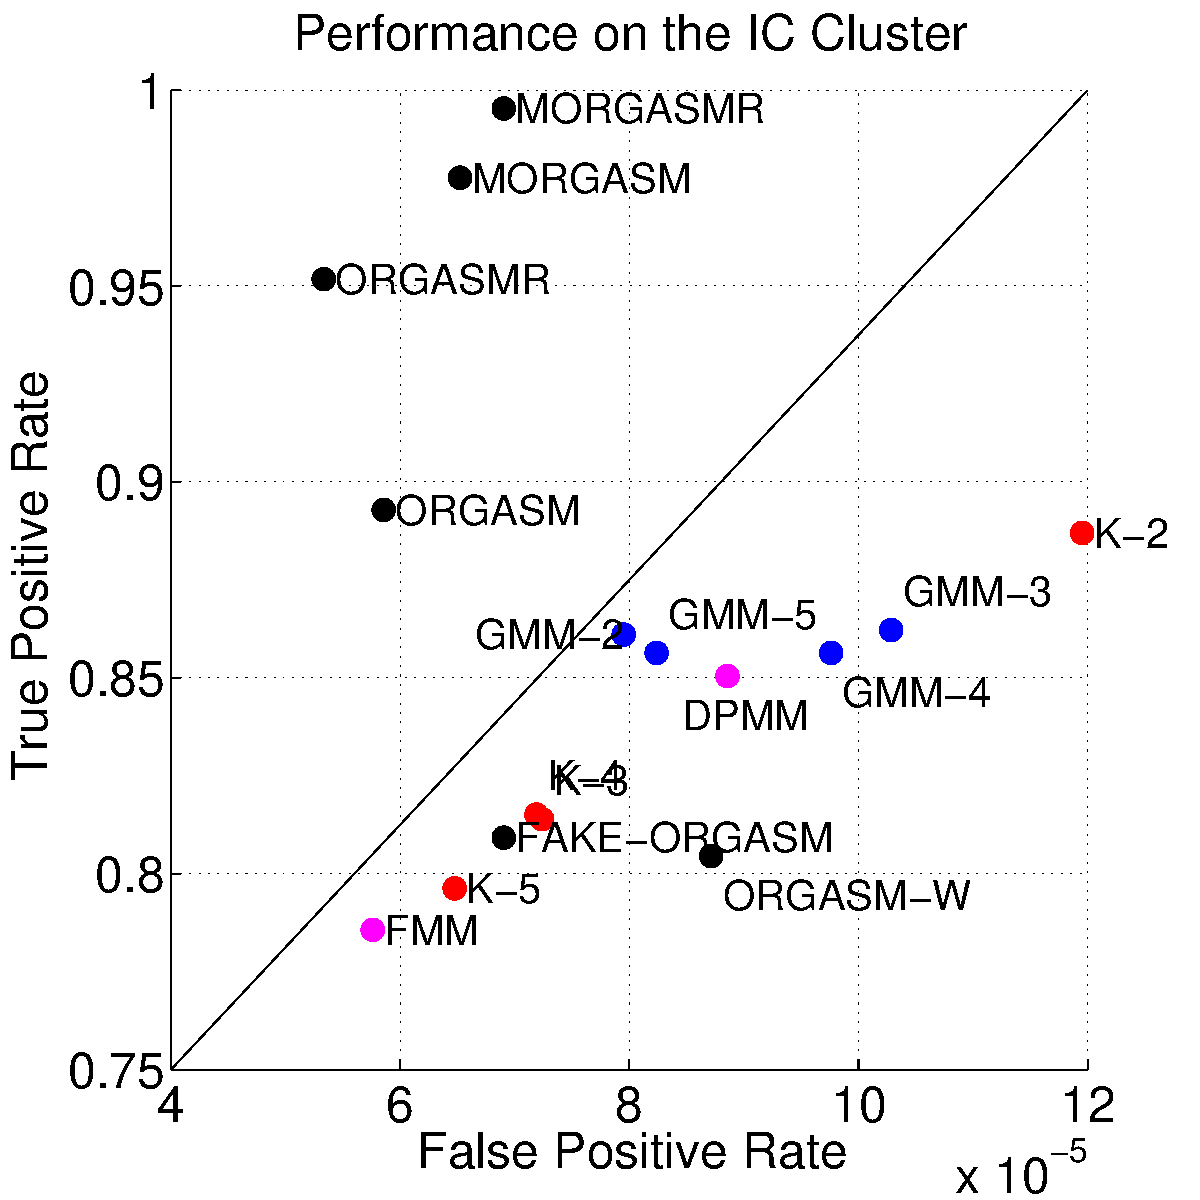
\includegraphics[width=\textwidth]{../figs/truefalsepositive}
% \caption{Schematic of our Generative Model.}
% \label{fig:schmetic}
% \end{figure}
% \end{center}
% 
{The total signal recorded from any electrode  is the superposition of the outputs of all neurons. Assume for the moment there are $N$
neurons, and define $\mc{T} \equiv \cup_{i \in [N]} \mc{T}_i$ as
the (ordered) union of the spike times of all neurons. 
Let $\tau_l \in \mc{T}$ indicate the time of $l^{th}$ overall spike, whereas $\tau_{ij} \in \mc{T}_i$ is the time of the $j^{th}$ spike of neuron $i$.
%To map elements  $\tau_{ij} \in \mc{T}_i$ to elements  $\tau_l \in \mc{T}$,   
This defines a pair of mappings: $\nu:[|\mc{T}|]\rightarrow [N]$, and $p:[|\mc{T}|]\rightarrow \mc{T}_{\nu_i}$, with %$(i = \nu(l))$, , which maps from the $j^{th}$ spikes of neuron $i$ to the $l^{th}$ overall spike.
$\tau_l = \tau_{\nu_l p_l}$. 
%\jovo{i don't think the square brackets around $\mc{T}$ are correct, we are mapping from the set of spikes, not the number of spikes, right?} 
In words, $\nu_l \in N$ is the neuron to which the $l^{th}$ element of $\mc{T}$ belongs, 
while $p_l$ indexes this spike in the spike train $\mc{T}_{\nu_l}$.
%\jovo{``position'' is weird to me.  can we say: ``indexes which spike of neuron $\nu_l$'', or something like that?}.
Let $\bth_l \equiv (\mb{\mu}_l, \Sigma_l)$ be the neuron parameter associated with spike $l$, so that $\bth_l = \bth^*_{\nu_l}$. 
Finally, define $\by_l \equiv (y_{l1}, \ldots, y_{lK})\T \equiv \tby_{\nu_j p_j}$ as the weight vector of spike $\tau_l$. Then, we have that}
% \begin{subequations}
\begin{align}
  x(t) &= \sum_{i \in [N]} x_{i}(t) =   \sum_{l \in |\mc{T}|} \sum_{k \in [K]} y_{lk} \mathsf{d}_k(t - \tau_{l}), \qquad %\label{eq:spk_sup} \\
% \intertext{where}
  \text{ where } \by_{l}  \sim \mathsf{N}_K(\mb{\mu}_{l}, \Sigma_{l}). \label{eq:spk}
\end{align}
% \end{subequations}
% 
From the superposition property of the Poisson process \citep{kingman93}, the overall spiking activity $\mc{T}$ is 
Poisson with rate $\Lambda = \sum_{i \in [N]} \lambda_i$. Each event $\tau_l \in \mc{T}$ has a pair of labels, its neuron parameter
$\bth_l \equiv (\mb{\mu}_l, \Sigma_l)$, and $\by_l$, the weight-vector characterizing the spike shape. We view these weight-vectors as the ``marks'' of a 
marked Poisson process $\mc{T}$.  From the properties of the Poisson process, we have that the marks $\bth_l$ are drawn i.i.d. from a probability measure:
$\quad  \mathsf{G}(\dd \bth) = 1/\Lambda\sum_{i \in [N]} \lambda_i \delta_{\bth^*_i}$.
\vspace{-.27in}
\begin{align}
    \label{eq:mark_distr}
\end{align}
Note that with probability one, the neurons have distinct parameters, so that the mark $\bth_l$ associated with spike $l$ identifies the
neuron which produced it: $\mathsf{G}(\bth_l = \bth^*_i) = \mathsf{P}(\nu_l= i) = \lambda_i/$$\Lambda$. Given $\bth_l$, $\by_l$ is distributed as in
Eq.~\eqref{eq:spk}. The output waveform $x(t)$ is then a linear functional of this marked Poisson process. % (Eq.~\eqref{eq:spk_sup}). 

%\vspace{-.1in}
\subsection{Completely random measures (CRMs)}
%\vspace{-.1in}

%The previous section assumed a known number of neurons $N$; 
In practice, the number of neurons driving the recorded activity is unknown. We do not wish to bound this number \emph{a priori}, 
moreover we expect this number to increase as we 
record over longer intervals. This suggests a nonparametric Bayesian approach: allow the \emph{total} 
number of underlying neurons to be infinite.
Over any finite interval, only a finite subset of these will be \emph{active}, and these dominate spiking activity over any interval.
This elegant and flexible modeling approach allows the data to suggest how many neurons are active, and has already proved 
successful in neuroscience applications \citep{WoodBla2008}.
%where we allow the number of neurons to be infinite.
%this leads to 
%While the number of neurons observed over any finite observation interval is finite, this number increases with the observation interval. 
%This makes sense in a biological context, in that as we record for longer (e.g., days, weeks, or months even), certain neurons will die or drop-out, and others will appear, simply by virtue of the electrodes moving, for example. 
 %, moreover the total rate $\Lambda$ of all neurons must also be finite.
%the total rate $\Lambda$ must 
%also be finite. Moreover, we want this to be dominated by a few $\lambda_i$: the corresponding neurons contribute the majority of the spiking
%activity in the observation interval. 
% A natural framework that captures our  modeling requirements is that of \emph{completely random measures} (CRMs) \citep{Kingman:PJM67}.
% CRMs are stochastic processes that form flexible and convenient priors over
% infinite dimensional objects like probability distributions \citep{JamesLP09}, hazard functions \citep{Hjo1990}, latent features \citep{ThiJor2007}. 
% These have been well studied in the Bayesian nonparametrics and machine learning communities, and there is a wealth of literature on
% theoretical properties, as well as posterior computation.
% 
% Recall that each neuron is characterized by a pair of parameters $(\lambda_i, \bth^*_i)$; characterizing the distribution over spike times 
% and shapes respectively. With Eq.~\eqref{eq:mark_distr} in mind, we map the infinite collection of pairs $\{(\lambda_i, \bth^*_i)\}$ to an atomic measure on $\Theta$:
% $\quad \mathsf{\Lambda}(\dd \bth) = \sum_{i=1}^{\infty} \lambda_i \delta_{\bth^*_i}$.
% 
% =======
We use the framework of \emph{completely random measures} (CRMs) \citep{Kingman:PJM67} to model our data.
%CRMs are stochastic processes that form flexible and convenient priors over
%infinite dimensional objects like probability distributions \citep{JamesLP09}, hazard functions \citep{Hjo1990}, latent features \citep{ThiJor2007}. 
CRMs have been well studied in the Bayesian nonparametrics community, and there is a wealth of literature on
theoretical properties, as well as posterior computation; see eg.\ \citep{JamesLP09, Hjo1990, ThiJor2007}. 
%Recall that each neuron is characterized by a pair of parameters $(\lambda_i, \bth^*_i)$; characterizing the distribution over spike times 
%and shapes respectively. 
With Eq.~\eqref{eq:mark_distr} in mind, and recalling that each neuron is characterized by a pair of parameters $(\lambda_i, \bth^*_i)$,
we map the infinite collection of pairs $\{(\lambda_i, \bth^*_i)\}$ to an random measure on $\Theta$:
$\ \  \Lambda(\dd \bth) = \sum_{i=1}^{\infty} \lambda_i \delta_{\bth^*_i}$.
% >>>>>>> ff0f5b20cd09ef2d570aa2ed8ea5c6d04356249f

For a CRM, the distribution over measures is induced by distributions
over the infinite sequence of weights, and the infinite sequence of their locations. 
The weights $\lambda_i$ are the jumps of a \Levy process \citep{Sato90}, and their distribution is characterized by a 
\Levy measure $\rho(\lambda)$. The locations $\bth^*_i$ are drawn i.i.d.\  from a base probability measure $H(\bth^*)$.
As is typical, we assume these to be independent. % (though this is not necessary). 
%{\color{green} if there's space, I
%can elaborate on the construction of the CRM from its Levy measure, though this is not necessary}

We set the \Levy measure $\rho(\lambda) = \alpha \lambda^{-1}\exp(-\lambda)$,
resulting in a CRM called the Gamma process ($\Gamma$P) \citep{applebaum2004}. 
The Gamma process has the convenient property that the 
total rate $\Lambda \equiv \mathsf{\Lambda}(\Theta) = \sum_{i=1}^{\infty} \lambda_i$ is Gamma distributed (and thus conjugate to the Poisson process prior on $\mc{T}$).
%\footnote{We abuse notation by using $\Lambda$ to denote both the measure as well as the total measure of $\Theta}
%The Gamma distribution has shape parameter $1$ and scale parameter $\alpha$.  Since this is finite almost surely, so too is $\mc{T}$. 
The Gamma process is also closely connected with the Dirichlet process \citep{Ferguson73}, which will prove useful
later on.
Other \Levy measures can be used to capture greater uncertainty in the number of neurons active in any finite interval, or to model
% To complete the specification on the Gamma process, we choose a base-measure $\mathsf{H}(\bth^*)$.
% %Recalling that $\bth^* \equiv (\mu^*, \Sigma^*)$ gives the mean and variance of the weight-vector $\by^*$ of a neuron, 
% We set $\mathsf{H}(\bth^*)$ 
% to the conjugate normal-Wishart distribution with parameters $\phi$. 
% =======
To complete the specification on the Gamma process, %we choose a base-measure $H(\bth^*)$.
%Recalling that $\bth^* \equiv (\mu^*, \Sigma^*)$ gives the mean and variance of the weight-vector $\by^*$ of a neuron, 
we set $H(\bth^*)$ 
to the conjugate normal-Wishart distribution with hyperparameters $\phi$.
% >>>>>>> ff0f5b20cd09ef2d570aa2ed8ea5c6d04356249f
%Our overall model is then:
%\begin{subequations}
%\begin{align}
%  \mc{T}_i\ \  &\sim \mathsf{PP}(\lambda_i) \quad i \in \NN, \quad &\text{ where } \mathsf{\Lambda}(\cdot)&=\sum_{i=1}^{\infty} \lambda_i \delta_{\theta^*_i} \sim \Gamma \text{P}(\alpha, \mathsf{H}(\cdot| {\phi})), \\ %\mathcal{NW}(\mu, \Sigma)) \\ \\
%\vspace{-.8in}
%  x_i(t) &= \sum_{j = 1}^{|\mc{T}_i|}  \sum_{k = 1}^{K} y^*_{ijk} \mathsf{d}_k(t - \tau_{ij}), \quad &\text{ where }\by^*_{ij}  &\sim \mathsf{N}_K(\mb{\mu}^*_i, \Sigma^*_i) \quad i,j \in \NN, \\
%  x(t)   &= \sum_{i=1}^{\infty} x_i(t) + \eps_t, \quad &\text{ where at any time $t$, } \eps_t &\sim \mathsf{N}(0,\Sigma_x) \text{ independently}
%\end{align}
%\end{subequations}

%Each spike of each neuron is associated with a time $e$ and a weight vector $y$, and one can view the model above as a doubly stochastic Poisson
%process on the product space. 
% 
%\jovo{perhaps it is standard, but you sample $\Lambda$ and then the next line you have $\lambda_i$, but no explanation for how you from $\Lambda$ to $\lambda_i$. i also am confused as to why $\phi$ is a subscript on $H$, rather than in the $(\cdot)$}
%Atom $i$ of the CRM corresponds to a neuron with parameters $(\lambda_i, \theta^*_i)$. 
It is easy to directly specify the resulting continuous-time model, we provide the equations in the Supplementary material. 
However it is more convenient to represent the model using the marked Poisson process of Eq.~\eqref{eq:spk}. % and \eqref{eq:spk_shape}. 
Then, the overall process $\mc{T}$ is a rate $\Lambda$ Poisson process,
and under a Gamma process prior, $\Lambda$ is Gamma$(\alpha,1)$ distributed %with shape and scale parameters $\alpha$ and $1$ respectively 
\citep{Ferguson73}.
As we saw (Eq.~\eqref{eq:mark_distr}), the labels $\bth_i$ assigning events to neurons are drawn i.i.d. from a normalized Gamma 
process: % $\mathsf{G}(\dd \bth)$:
%\vspace{-.2in}
%\begin{align}
$ \mathsf{G}(\dd \bth) = \frac{1}{\Lambda} \sum_{l=1}^{\infty} \lambda_l$.
%\end{align}

$\mathsf{G}(\dd \bth)$ is a random probability measure (RPM) called a \emph{normalized random measure} \citep{JamesLP09}. Crucially, a 
normalized Gamma process is the Dirichlet process (DP) \citep{Ferguson73}, so that 
the spike parameters $\bth$ are i.i.d.\ draws with a DP-distributed RPM.
For the $l^{th}$ spike in $\mc{T}$, its shape vector is drawn from a normal distribution
with parameters $(\mb{\mu}_{l}, \Sigma_{l})$: these are thus
draws from a DP mixture model (DPMM) of Gaussians \citep{Lo1984}.

% <<<<<<< HEAD
% The connection with the DP allows us to simplify the representation of our model. In particular, we exploit a remarkable property of the DP that
% allows us to integrate out the infinite-dimensional variable $\mathsf{G}(\cdot)$. The resulting marginal distribution over observations follows the so-called
%  Chinese restaurant process ($\mathsf{CRP}$) \citep{Pit2002a}. Under this scheme, the $l^{th}$ spike is assigned the same parameter as an earlier spike with probability 
% =======
%The connection with the DP allows us to simplify the representation of our model. In particular, 
We can exploit the connection with the DP to %a remarkable property of the DP that allows us to 
integrate out the infinite-dimensional measure $G(\cdot)$ (and thus $\Lambda(\cdot)$), and assign spikes to neurons via 
%. The resulting marginal distribution over observations follows 
the so-called Chinese restaurant process (CRP) \citep{Pit2002a}. Under this scheme, the $l^{th}$ spike is assigned the same parameter as an earlier spike with probability 
% >>>>>>> ff0f5b20cd09ef2d570aa2ed8ea5c6d04356249f
proportional to the number of earlier spikes having that parameter. It is assigned a new parameter (and thus, a new neuron is observed) with probability 
proportional to $\alpha$. Letting $C_t$ be the number of neurons observed until time $t$, and  $\mc{T}^t_i = \mc{T}_i \cap [0,t)$ be the times of spikes 
produced by neuron $i$ before time $t$,
we then have for spike $l$ at time $t = \tau_l$: 
\vspace{-.06in}
\begin{align}
 \bth_l = \bth^*_{\nu_l} \text{, where } 
  P({\nu_l} = i) & \propto 
  \begin{cases}
   |\mc{T}^t_i| \quad i \in \{1,\cdots, C_{t}\}, \\
   \alpha \quad\ i = C_{t} + 1, 
  \end{cases}  
\label{eq:crp_marg_pr}
\end{align}
%\footnote{Strictly speaking, the process we just described is called a P\'olya urn scheme \citep{BlaMac1973}; for simplicity, we do not distinguish between this and the \mathsf{CRP}.}.
This marginalization property of the DP allows us to integrate out the infinite-dimensional rate vector $\mathsf{\Lambda}(\cdot)$, and sequentially 
assign spikes to neurons based on the assignments of earlier spikes.
%is assigned (or equivalently, the parameter $\bth$ associated with that neuron). These marks are drawn from a probability measure 
%$\mathsf{G}(\dd \bth) = \frac{1}{R} R(\dd \bth)$. From the properties of the Gamma process, the probability measure $G$ a Dirichlet process, 
This requires one last property: for the Gamma process, the RPM $\mathsf{G}(\cdot)$ is independent of the total mass $\Lambda$. 
Consequently, the clustering of spikes (determined by $\mathsf{G}(\cdot)$) is independent of the rate $\Lambda$ at which they are produced. We then have
 the following model equivalent to the one above:
\begin{subequations}
\begin{align}
  \mc{T} &\sim \PP(\Lambda), \qquad &\text{ where } \Lambda  &\sim \mathsf{\Gamma P}(\alpha, 1),
   \\
  \by_l &\sim \mathsf{N}_K(\mb{\mu}_{l}, \Sigma_{l}), \qquad &\text{ where } (\mb{\mu}_{l}, \Sigma_{l})  &\sim {\mathsf{CRP}}(\alpha, \mathsf{H}_{\phi}(\cdot)), \quad  l \in [|\mc{T}|],   \label{eq:CRP}\\
   % (\mb{\mu}_{l}, \Sigma_{l}) &\equiv \bth_l,  &\text{ where } \bth_l &\sim \text{\mathsf{CRP}}(\alpha, \mathsf{H}_{\phi}(\cdot)), \quad l \in [|\mc{T}|],   \label{eq:\mathsf{CRP}}\\
  x(t) &=   \textstyle{\sum_{l \in |\mc{T}|}} \sum_{k \in [K]} y_{lk} \mathsf{d}_k(t - \tau_{l}) + \eps_t  &\text{ where }  \eps_t &\iid \mathsf{N}(0,\sigma^2),  \,  l \in [|\mc{T}|].   \label{eq:CRP_mix}
\end{align} \label{eq:marked_pp}
\end{subequations}
% Unlike most applications which observe the outputs of a $\mathsf{CRP}$, our observation at any time $t$ is a convolution-like function of the $\mathsf{CRP}$ outputs of all
% earlier times. Consequently, we cannot directly apply standard techniques for posterior inference. In \S \ref{sec:inf}, we develop a novel online 
% algorithm for posterior inference; first, we provide a discrete-time approximation to our model.
% =======
%Unlike most applications which observe the outputs of a CRP, our observation at any time $t$ is a convolution-like function of the CRP outputs of all
%earlier times. Consequently, we cannot directly apply standard techniques for posterior inference. In \S \ref{sec:inf}, we develop a novel online 
%algorithm for posterior inference; first, we provide a discrete-time approximation to our model.
% >>>>>>> ff0f5b20cd09ef2d570aa2ed8ea5c6d04356249f

%For neuron $i$, the sequence of spike times is distributed as a Poisson process with random rate $\lambda_i$.
%Each event $\tau_{ij}$ is associated with a mark or label $y_{ij}$ drawn from a normal distribution (again, with random parameters).
%More broadly, we can view the superposed process $\mc{T}$ as a rate $\Lambda$ Poisson process, with each event having a pair of marks, the neuron identity $i$,
%and weight $y$. From the properties of the Gamma process, the pair form a draw from a Dirichlet process.
%Our data is in a form that makes discrete-time modeling more natural, and an approach now is
%one based on the Beta process-binomial process.

%\vspace{-.1in}
% =======
\vspace{-.2in}
% >>>>>>> ff0f5b20cd09ef2d570aa2ed8ea5c6d04356249f
\subsection{A discrete-time approximation}
% \vspace{-.1in}
The previous subsections modeled the continuous-time voltage output of a neuron. Our data on the other hand consists of recordings
at a discrete set of times. While it is possible to make inferences about the continuous-time process underlying these discrete recordings,
in this paper, %for simplicity, 
we restrict ourselves to the discrete case. %We thus provide a discrete-time approximation to the model above. 
The marked Poisson process characterization of Eq.\ \ref{eq:marked_pp} leads to a simple
discrete-time approximation of our model.

Recall first the Bernoulli approximation to the Poisson process: a sample from a Poisson process with rate $\Lambda$ can be approximated by discretizing
time at a granularity $\Delta$, and assigning each bin an event independently with probability $\Lambda\Delta$ (the accuracy of the approximation increasing 
as $\Delta$ tends to $0$).
%
%This suggests the following approximation at a time resolution $\Delta$. Draw the random Poisson process rate $\Lambda$ drawn from a Gamma$(1,\alpha)$ 
%distribution. Simultaneously, draw a random probability measure
% $G$ from a Dirichlet process. Assign an event to an interval independently with probability $\Lambda\Delta$, and to each event, assign a random mark drawn 
To approximate the \emph{marked} Poisson process $\mc{T}$, all that is additionally required is to assign marks $\bth_i$ and $\by_i$ to each event 
in the Bernoulli approximation. Following Eqs.~\eqref{eq:CRP} and \eqref{eq:CRP_mix}, the $\bth_l$'s are distributed according
to a Chinese restaurant process, while each $\by_l$ is drawn from a normal distribution parametrized by the corresponding $\bth_l$. We discretize the 
elements of dictionary $\mathsf{d}_k \equiv \{\mathsf{d}_k(t)\}_{t \in (0,T)}$ as well, %defining a mapping from $L_2$ to $\Real^L$ 
yielding discrete dictionary elements 
$\mt{\bd}_{k,:}=(\mt{d}_k[1], \ldots, \mt{d}_k[L])\T$. These form the rows of a ${K \times L}$ matrix $\mt{\bD}$ (we call its columns
$\mt{\bd}_{:,h}$). The shape of the $j^{th}$ spike is now a vector of length $L$, and for a weight vector
$\by$, is given by $\mt{\bD} \by$.

We can simplify notation a little for the discrete-time model. Let $t$ index time-bins (so that for an observation interval of length 
$T$, $t \in [T/\Delta]$).
Let the binary variable $\mt{z}_t$ indicate whether or not a spike in present in time bin $t$ (recall that 
$\mt{z}_t \sim \text{Bernoulli}(\Lambda \Delta)$). Let
$\mt{\nu}_t$ and $\mt{\theta}_t$ be the neuron and neuron parameter associate with time bin $t$, and let $\mt{\by}_t$ be its weight-vector. 
If there is a spike associated with that bin (i.e.\ 
$\mt{z}_t = 1$), then these are the marks of that spike, otherwise we ignore them.
Then the output at time $t$, $x_t$ is given by
%\begin{align}
$\quad  x_t = \sum_{h = 1}^L \mt{z}_{t-h} \mathsf{\bd}_{:,h}^{\T} \mt{\by}_{t-h-1} + \eps_t \text{,\quad where $\eps_t \iid \mathsf{N}(0,\sigma^2)$.}$ 
%\end{align}
% \vspace{-.1in}
\subsection{Correlations in time and across electrodes}
% \vspace{-.1in}
So far, so simplicity, we restricted our model to recordings from a single channel. We now describe the full model we use in the experiments for
multichannel recordings. Every spike affects the recordings at all channel, however, we allow the spike shape to vary across channels. 
For spike $l$ in channel $m$, call the weight-vector $\by^m_l$. All these vectors must be correlated as they correspond to the same spike; we do this 
simply by concatenating the set of vectors into
a single $MK$-element vector $\by_l = (\by^1_l;\cdots;\by^M_l)$, and modeling this as a multivariate normal. In principle, one might expect the associated 
covariance matrix to possess a block structure (corresponding to subvector associated with each channel); however, rather than building this into the model,
we allow the data to inform us about any such structure.

We also relax the requirement that the parameters $\bth^*$ of each neuron remain constant, and instead allow $\mb{\mu}^*$, the mean of the weight-vector,
to evolve with time (we keep the covariance parameter $\mb{\Sigma}^*_i$ fixed, however). Such flexibility can capture effects like changing cell 
characteristics or moving electrodes.
We model the time-evolution of the mean vector of a neuron as a realization of a Gaussian process (GP) \citep{RasWil2006}. A consequence is that the 
means remain marginally Gaussian distributed at any time, on the other hand correlation between means across time is determined by the choice 
of the GP covariance kernel.
We choose a stationary Markov kernel (where covariance decays exponentially with time); in discrete-time, this corresponds to a simple first-order 
autoregressive process. With $\mb{A} \in \mathbb{R}^{K \times K}$ the transition matrix, and $\mb{r}_t \in \mathbb{R}^K$, 
independent and Gaussian {innovations}, we have
Algorithm \ref{alg:gen_proc} in the supplementary material summarizes the generative mechanism of the data for the full discrete-time model.


%The first is the inclusion of measurement noise: {\color{red} Biology?}. Let $\eps_t$ be the noise at time $t$, we model this as independent, additive and Gaussian.
%However, rather than modeling the noise as independent across time, we model it as a first-order autoregressive process. This can capture
%effects like the movement of electrodes during the experiment. 
% 
% \begin{align}
  $\mb{\mu}^*_{t+1} = \mathbf{B} \mb{\mu}^*_t + \mathbf{r}_t$.
% \end{align}
Where we previously had a DP mixture of Gaussians, we now have a DP mixture of GPs. Each neuron is now associated with a vector-valued function 
$\bth^*(\cdot)$, rather than a constant. When a spike at time $\tau_l$ is assigned to neuron $i$, it is assigned a weight-vector $\by_l$ drawn from a 
Gaussian with mean $\mb{\mu}^*_i(\tau_l)$. %Following \citep{wood2009}, a useful extension is to also allow the neuron assignment probabilities to evolve 
%(corresponding to a time-varying Gamma process \citep{RaoTeh2009a}); we leave this for future work. 
In a similar way, we also induce correlations in the noise, we model this as an AR process with transition matrix $\mathbf{B}$.



% \vspace{-.1in}
\section{Inference} \label{sec:inf}
% \vspace{-.1in}
\newcommand{\tx}{\tilde{x}}
\newcommand{\resx}{\delta{\bx}^L}


We now address the problem of posterior inference over the latent variables given the matrix $\bX$ of multielectrode recordings. 
%Unsurprisingly, exact inference is intractable, and we have to resort to approximating the posterior distribution.
There exists a vast literature on computational approaches to posterior inference for Bayesian nonparametric models, especially so for models based on the 
Dirichlet process.
Traditional approaches are sampling-based, typically involving Markov chain Monte Carlo techniques (see eg.\ \citep{Nea2000, IshJam2001}), 
and recently there has also been work on constructing deterministic approximations to the intractable posterior (eg.\ \citep{BleJor2006, MinGha2003}).
Our problem is complicated by two additional factors. The first is the convolutional nature of our observation process, 
where at each time,
we observe a function of the previous observations drawn from the DP mixture model. This is in contrast to the usual situation where one directly observes 
the DPMM outputs themselves.
The second complication is a computational requirement: typical inference schemes are batch methods that are slow and computationally expensive. 
Our ultimate goal, on the other hand, is to perform inference in real time, making these approaches are unsuitable for our purposes.

Keeping the latter objective in mind, we develop an online algorithm for posterior inference. Our algorithm is based on the sequential update and
greedy search (SUGS) algorithm of
\citep{WangDun2009}, though that work was concerned with the usual case of i.i.d.\ observations from a DPMM. We generalize SUGS to our 
observation process, also accounting for the time-evolution of the cluster parameters.

Below, we describe an iteration of our algorithm for the case a single electrode; %Most steps are repeated across all electrodes; 
%we will point out when the need for anything more complicated arises. 
generalizing to the multielectrode case is straightforward. 
At a high level, at time $t$, our algorithm maintains the set of times of the spikes it has inferred from the observations so far. It also maintains
the identities of the neurons that it assigned each of these spikes to, as well as the weight vectors determining the shapes of the associated spike 
waveforms. We indicate these point estimates with the hat operator, so, for example $\mh{\mc{T}}^t_i$ is the set of estimated spike times before time $t$ assigned
to neuron $i$. The algorithm also keeps a set of posterior distributions $q_{it}(\theta^*_i)$ where $i$ spans over the
set of neurons associated with the spikes seen so far (i.e.\ $i \in [\mh{C}_t]$). 
For each $i$, $q_{it}(\theta^*_i)$ approximates the distribution over the parameters 
$\theta_i^* \equiv (\mu_i^*, \Sigma_i^*)$ of neuron $i$ given the observations until time $t$. 

Having identified the location and shape of spikes from earlier times, we can calculate their contribution to the recordings 
$\bx^L_t \equiv (x_{t+1},\cdots, x_{t+L})$.
Recalling that the basis functions $\bD$, and thus all spike waveforms, span $L$ time bins, the residual at time $t$ is then given by
\begin{align}
  \resx_t = \bx^L_t - \sum_{h=1}^L \bD\mh{\by}_{t-h} \label{eq:resid}
\end{align}

We treat the residual $\resx_{t+1}$ as an observation from a DP mixture model, and use this to make a hard decision about whether or not this was produced 
by an underlying spike, what neuron that spike belongs 
to (one of the earlier neurons or a new neuron), and what the shape of the associated spike waveform is. The latter is used to calculate
$q_{i,t+1}(\theta^*_i)$, the new distribution over neuron parameters at time $t+1$. Our algorithm proceeds recursively in this manner. 


%Let $z_t$ indicate whether or not a spike is present at time $t$, with $\by_t$ giving its shape, and $\nu_t$ its associated neuron. 
For the first step we decide whether or not there is a spike underlying the residual by applying Bayes' rule,
\begin{align}
  P(z_t = 1 | \resx_t)  &\propto P(z_t = 1,  \resx_t) = \sum_{\nu_t = 1}^{\mh{C}_{t-1}+1} P(\resx_t, {\nu_t} | z_t = 1) P(z_t = 1) \label{eq:spk_prob}\\
\intertext{$P({\nu_t} = i | z_t = 1)$ follows from the CRP update rule (equation \eqref{eq:crp_marg_pr}), while}
  P(\resx_t | {\nu_t = i} , z_t = 1) &= \int_{\Theta} P(\resx_t | \theta_t) q_{it} (\theta_t) \dd \theta_t  \label{eq:norm_nw}
\end{align}
Here,  $P(\resx_t | \theta_t)$ is just the normal distribution, while we restrict $q_{it}(\cdot)$ be the 
normal-Wishart distribution. % with parameters 
We can then evaluate integral \eqref{eq:norm_nw}, and then summation \eqref{eq:spk_prob} to calculate $P(z_t = 1 | \resx_t)$. 
If this exceeds a threshold of $0.5$ we decide that there is a spike present at time $t$, otherwise, we set $z_t = 0$.
Observe that making this decision involves marginalizing over all possible cluster assignments $\nu_t$, and all values of the weight vector $\by_t$.
On the other hand, having decided that a spike is present , we simplify matters collapsing these posterior distributions to point estimates 
$\mh{\nu}_t$ and $\mh{\by}_t$. Both are obtained from their MAP values. 

Given these point estimates, we can update the posterior distribution over parameters of cluster $\mh{\nu}_t$ to obtain $q_{i,t+1}$ from $q_{i,t}$; this
is straightforward because of conjugacy. 
We need to follow this up with an additional update step for the parameter distributions of \emph{all} clusters because of the AR process on the parameters.
This too is straightforward {\color{red} Get exact update rule. Hyperparameters}.

The online algorithms were all run with weakly informative parameters (\dec{add parameters once I get vinayak's notation}). The parameters were insensitive to minor changes.  Running time in unoptimized MATLAB code for 4 minutes of data was 31s was a single channel and 3 minutes for all 4 channels on a 3.2 GHz Intel Core i5 machine with 6 GB of memory.




\section{Experiments}

\subsection{Data}

We used two different datasets to demonstrate the efficacy of \smug.  First, the ever popular, publicly available HC1 dataset\footnote{http://crcns.org/data-sets/hc/hc-1/}
as described in \cite{Henze2000}.  We used the dataset d533101 that consisted of an extracellular tetrode and a single intracellular electrode.  The recording was made simultaneously on all electrodes and was set up such that the cell with the intracellular electrode was also recorded on the extracellular array implanted in the hippocampus of an anesthetized rat. The intracellular recording is relatively noiseless and gives nearly certain firing times of the intracellular neuron.  The extracellular recording contains the spike waveforms from the intracellular neuron as well as an unknown number of additional neurons.  The data is a 4-minute recording at a 10 kHz sampling rate.  

The second dataset comes from Michigan using Michigan probes\footnote{their website perhaps?}.  These data \jovo{@dec - need you here :).}



\jovo{@dec - same pre-processing for both?  regardless, need you to add it.}
We preprocessed with a high-pass filter at 800 Hz before we analyzed the time series.  To get the PCA decomposition, we used the spikes detected with a threshold (three times the standard deviation of the noise above the mean) in the first five seconds and used the top three principal components.  The noise standard deviation was estimated both over the first five seconds of the recording as well as the entire recording, and the estimate was nearly identical.  Our results were also robust to minor variations in the choice of the number of principal components.

Each algorithm gives a clustering of the detected spikes.  In this dataset, we only have a partial ground truth, so we can only verify accuracy for the neuron with the intracellular (IC) recording.  In these experiments, we define a detected spike to be an IC spike if the IC recording has a spike within 0.5 milliseconds (ms) of the detected spike in the extracellular recording.  We define the cluster with the greatest number of intracellular spikes as a the ``IC cluster''.   We refer to these data as ``partial ground truth data'', because we know the ground truth spike times for one of the neurons, but not all the others.  




\subsection{Bake-off Recipes}

We compare a number of variants of \smug, as well as several previously proposed methods, as described below.  The vanilla version of \smug\ operates on a single channel with colored noise.  When using multiple channels, we append an ``\sct{M}'' to obtain \sct{M}\smug.  When we model the mean of the waveforms as an auto-regressive process, we ``post-pend'' to obtain \smug\sct{R}.  
We compare these variants of \smug\ to Gaussian mixture models and k-means with N components (\sct{Gmm-N} and \sct{K-N}, respectively), where \sct{N} indicates the number of components.  Finally, we include a Focus Mixture Model (\sct{Fmm}) \cite{??}, a recently proposed Bayesian generative model with state-of-the-art performance.  Only \smug\ methods were online as we desired to compare to the state-of-the-art \emph{batch} algorithms which use all the data. 
% could not find any previous code available for online spike sorting, despite a small literature on the topic \cite{??}.  
Note that \smug\ algorithms used a dictionary learned from the first five seconds of data, whereas all other algorithms used a dictionary learned from the entire data set.  In either case, the dictionary consisted of the first five principal components of the matrix consisting of all waveforms from the thresholded voltage traces.  Supplementary Figure \ref{fig:waveforms} shows the two different dictionaries and the relative fraction of variance explained.

% 
% 
The single-channel experiments were all run on channel 2 (the results were nearly identical for all channels).  The spike detections for the offline methods used a threshold of three times the noise standard deviation \cite{Lewicki} (unless stated otherwise), and windowed at a size $L=30$.  For multichannel data, we concatenated the $M$ channels for each waveform to obtain a $M\times L$-dimensional vector.
%, and PCA was used to reduce the space to $K$=5 for the experiments. 

% \subsection{Results}

The online algorithms were all run with weakly informative parameters (\dec{add parameters once I get vinayak's notation}). The parameters were insensitive to minor changes.  Running time in unoptimized MATLAB code for 4 minutes of data was 31s was a single channel and 3 minutes for all 4 channels on a 3.2 GHz Intel Core i5 machine with 6 GB of memory.


\subsection{Performance on partial ground truth data}



The main empirical result of our contribution is that all variants of \smug\ detect more true positives with fewer false positives than any of the other algorithms on the partial ground truth data (see Figure \ref{hc1res}).  
Our improved sensitivity and specificity is \emph{despite} that \smug\ is fully online, whereas all the algorithms that we compare to are batch algorithms using all data for all spikes.   Note that all the comparison algorithms pre-process the data via thresholding at some constant (which we set to three standard deviations above the mean).  To assess the extent to which performance of \smug\ is due to \emph{not} thresholding, we implement \sct{Fake}-\smug, which thresholds the data.  Indeed, \sct{Fake}-\smug's performance is much like that of the batch algorithms.  To get uncertainty estimates, we split the data into ten random two minute segments and repeat this analysis. The results are qualitatively similar (see Supplementary Figure \ref{sfig:hc1res}).


One possible explanation for the relatively poor performance of the batch algorithms as compared to \smug\ is a poor choice of the important---but often overlooked---threshold parameter.  Figure \ref{fig:roc} shows the receiver operating characteristic (ROC) curve for the k-means algorithms as well as \smug\ and \sct{M}\smug\ (where \sct{M} indicates multichannel, see below for detail).  Although we typically run \smug\ without tuning parameters, the prior on $\Lambda$ sets the expected number of spikes, which we can vary in a kind of ``empirical Bayes'' strategy.  Indeed, the \smug\ curves are fully above the batch curves for all thresholds and priors, suggesting that regardless of which threshold one chooses for pre-processing, \smug\ always does better on these data than all the competitor algorithms.  Moreover, \smug\ which infers $\Lambda$ from the data (indicated by an \jovo{@dec - what symbol did you use here?}) is \jovo{@dec - does how good?}.

While the above analysis suggests that it is not the threshold that yields \smug\ improved performance; rather, it is \smug's ability to detect signals more reliably.  In the following, we provide evidence suggesting how several of \smug's key features are fundamental to this improvement.


 
\begin{center}
\begin{figure}
\begin{subfigure}[b]{.49\textwidth}
\centering
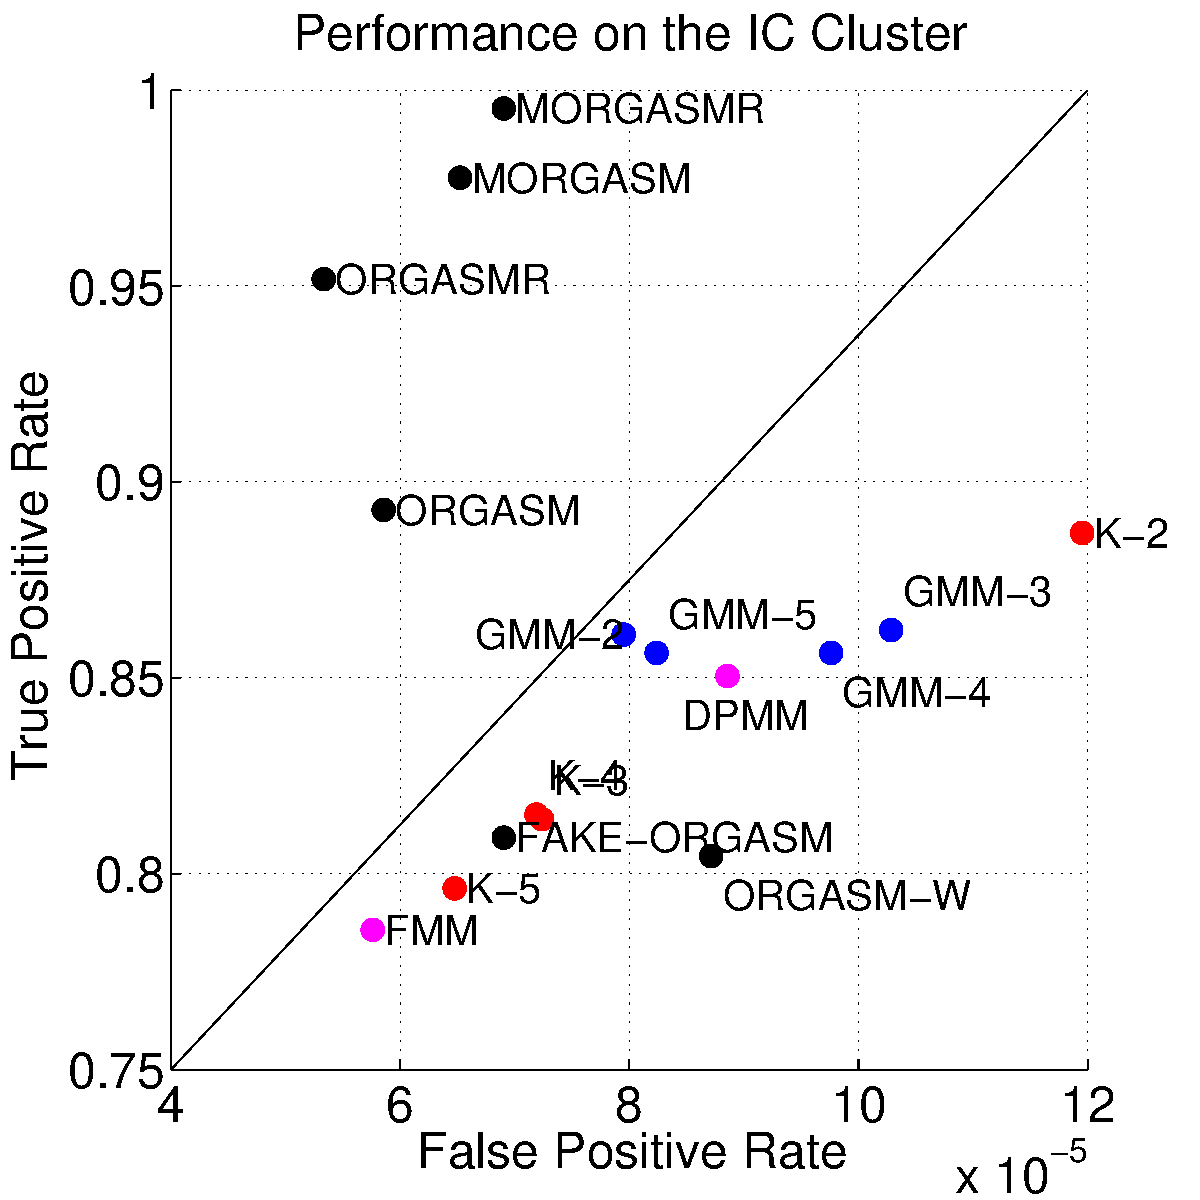
\includegraphics[width=\textwidth]{../figs/truefalsepositive.pdf}
\caption{}
\label{hc1res}
\end{subfigure}
\begin{subfigure}[b]{.49\textwidth}
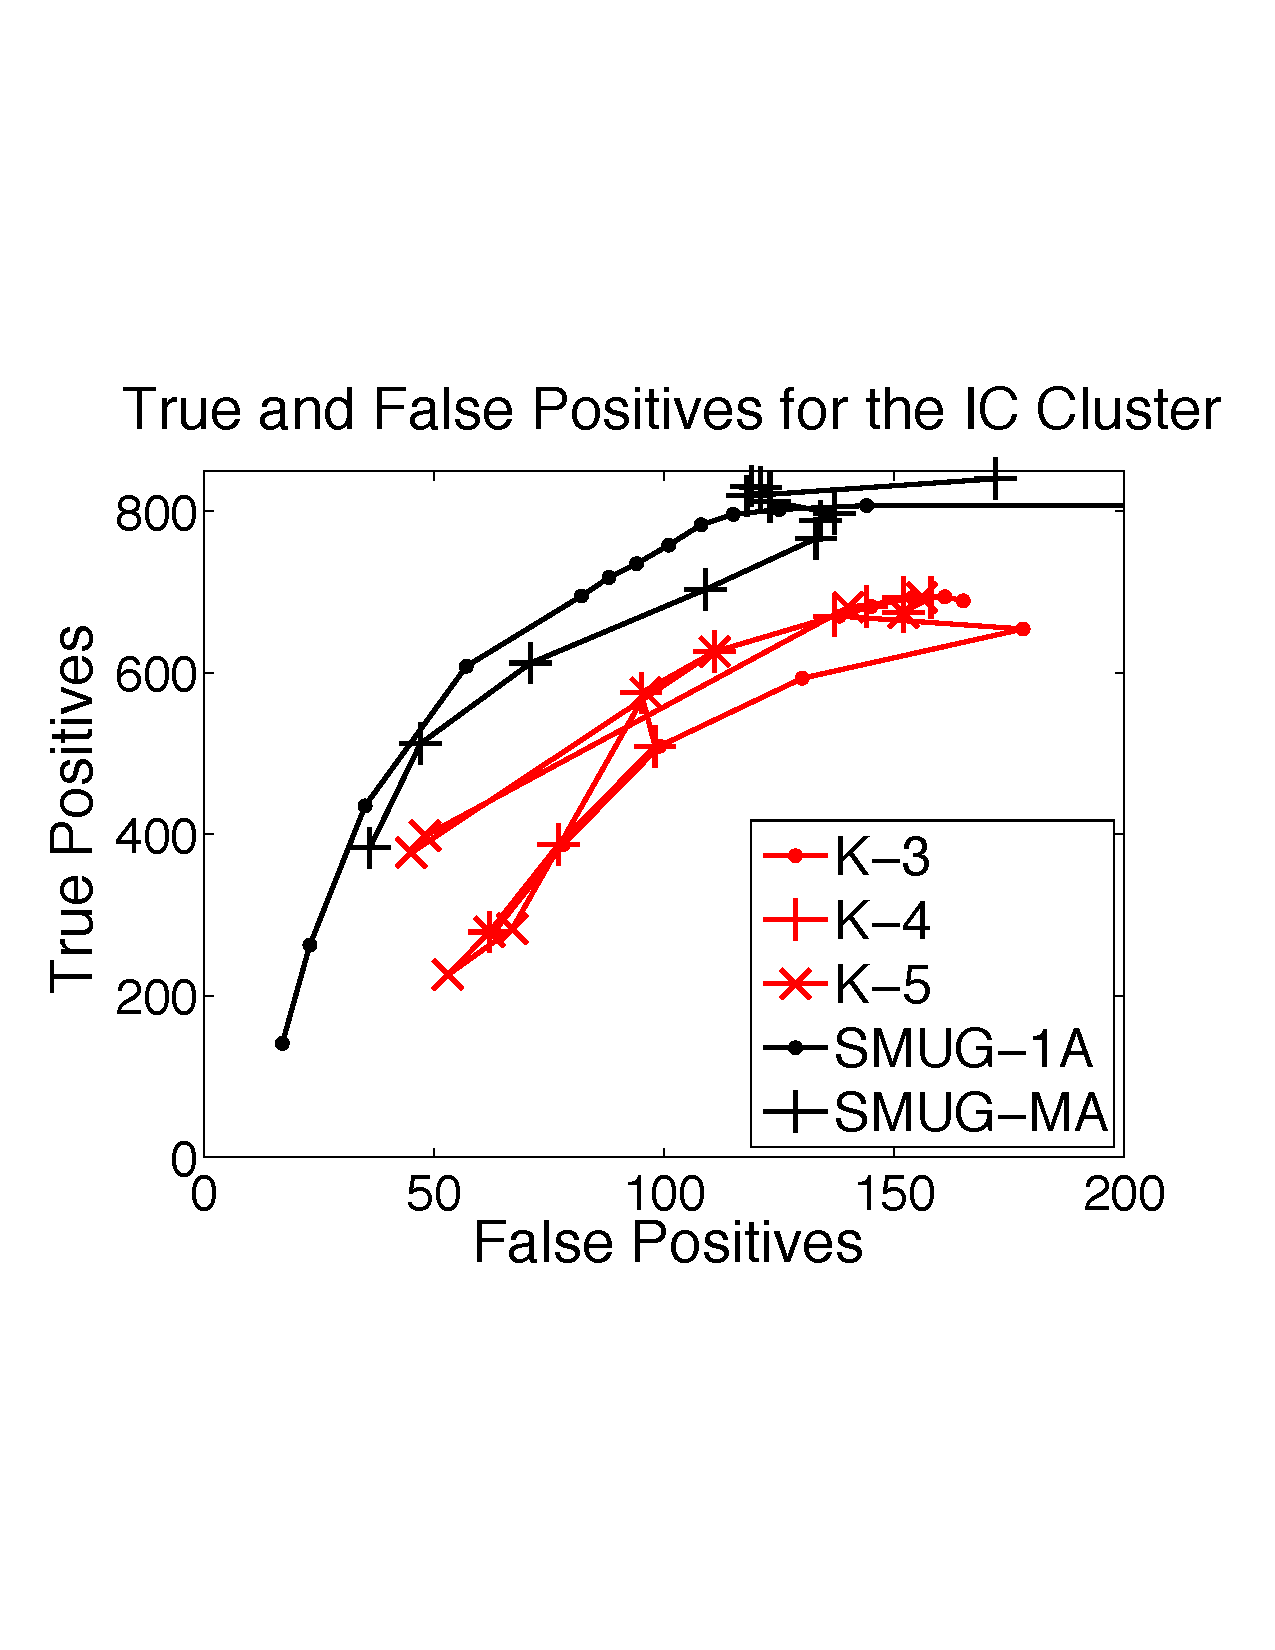
\includegraphics[width=\textwidth]{../figs/new/icroc.pdf}
\caption{}
\label{fig:roc}
\end{subfigure}
\caption{\smug\ achieves improved sensitivity and specificity over all competing methods on partial ground truth data (where true positives from one neuron are known from intracellular recordings).  
(a) True positive and false positive rates for all variants of \smug\ and several competing state-of-the-art \emph{batch} algorithms.  
(b) ROC curves demonstrating that both \sct{M}\smug\ and \smug\ outperform all competitor batch algorithms, regardless of threshold (including when we learn $\Lambda$ from the data, as indicated by a \jovo{*}).
\jovo{@dec - keep colors/symbols the same in the two panel, if possible.  maybe use a scheme where color indicates algorithm and shape indicates \# of components.  also, be consistent about "IC" cluster vs. "Intracellular" Cluster. and normalize, renaming axes XY Rate instead of only XY. (b) title should be ``ROC Curve Comparisons''}  
}
\end{figure}
\end{center}



\subsection{Overlapping Spike Detection}



A putative reason for the improved sensitivity and specificity of \smug\ over other algorithms is its ability to detect overlapping spikes.   When spikes overlap, although the result can accurately be modeled as a linear sum in voltage space, the resulting waveform often does not appear in any cluster in PC space (see \ref{Pillow2013}).  However, our online approach can readily find such overlapping spikes.  Figure \ref{fig:overlapping} shows one example of 135 examples where \smug\ believed that multiple waveforms were overlapping.  Indeed, it should be clear that by virtue of estimating the presence of multiple spikes, the residual squared error between the expected voltage and observed voltage shrinks.  Figure \ref{fig:resid} shows the density of the residual errors for all putative overlapping spikes.  The mass of this density is significantly smaller than the mass of the other scenarios.  Of all the true spikes that we detect, 37 of them we believe to be overlapping.  Thus, while it seems detecting overlapping spikes helps, it does not fully explain the improvements over the competitor algorithms.
\jovo{@jovo - add an actual statistical test test.} 


% It is possible for action potentials to fire close to simultaneously so that a given window would have 2 or move action potent ions.  It is possible for the algorithm to detect and fit overlapping spikes as they come in.  Out of the 3593 spikes detected by the algorithm, there are 124 pairs of overlapping spikes within 1 ms of one another (3.45\%).  An example of an overlapping waveform is shown in Figure \ref{overlapping}.


\begin{center}
\begin{SCfigure}[3]
\begin{subfigure}[b]{.3\textwidth}
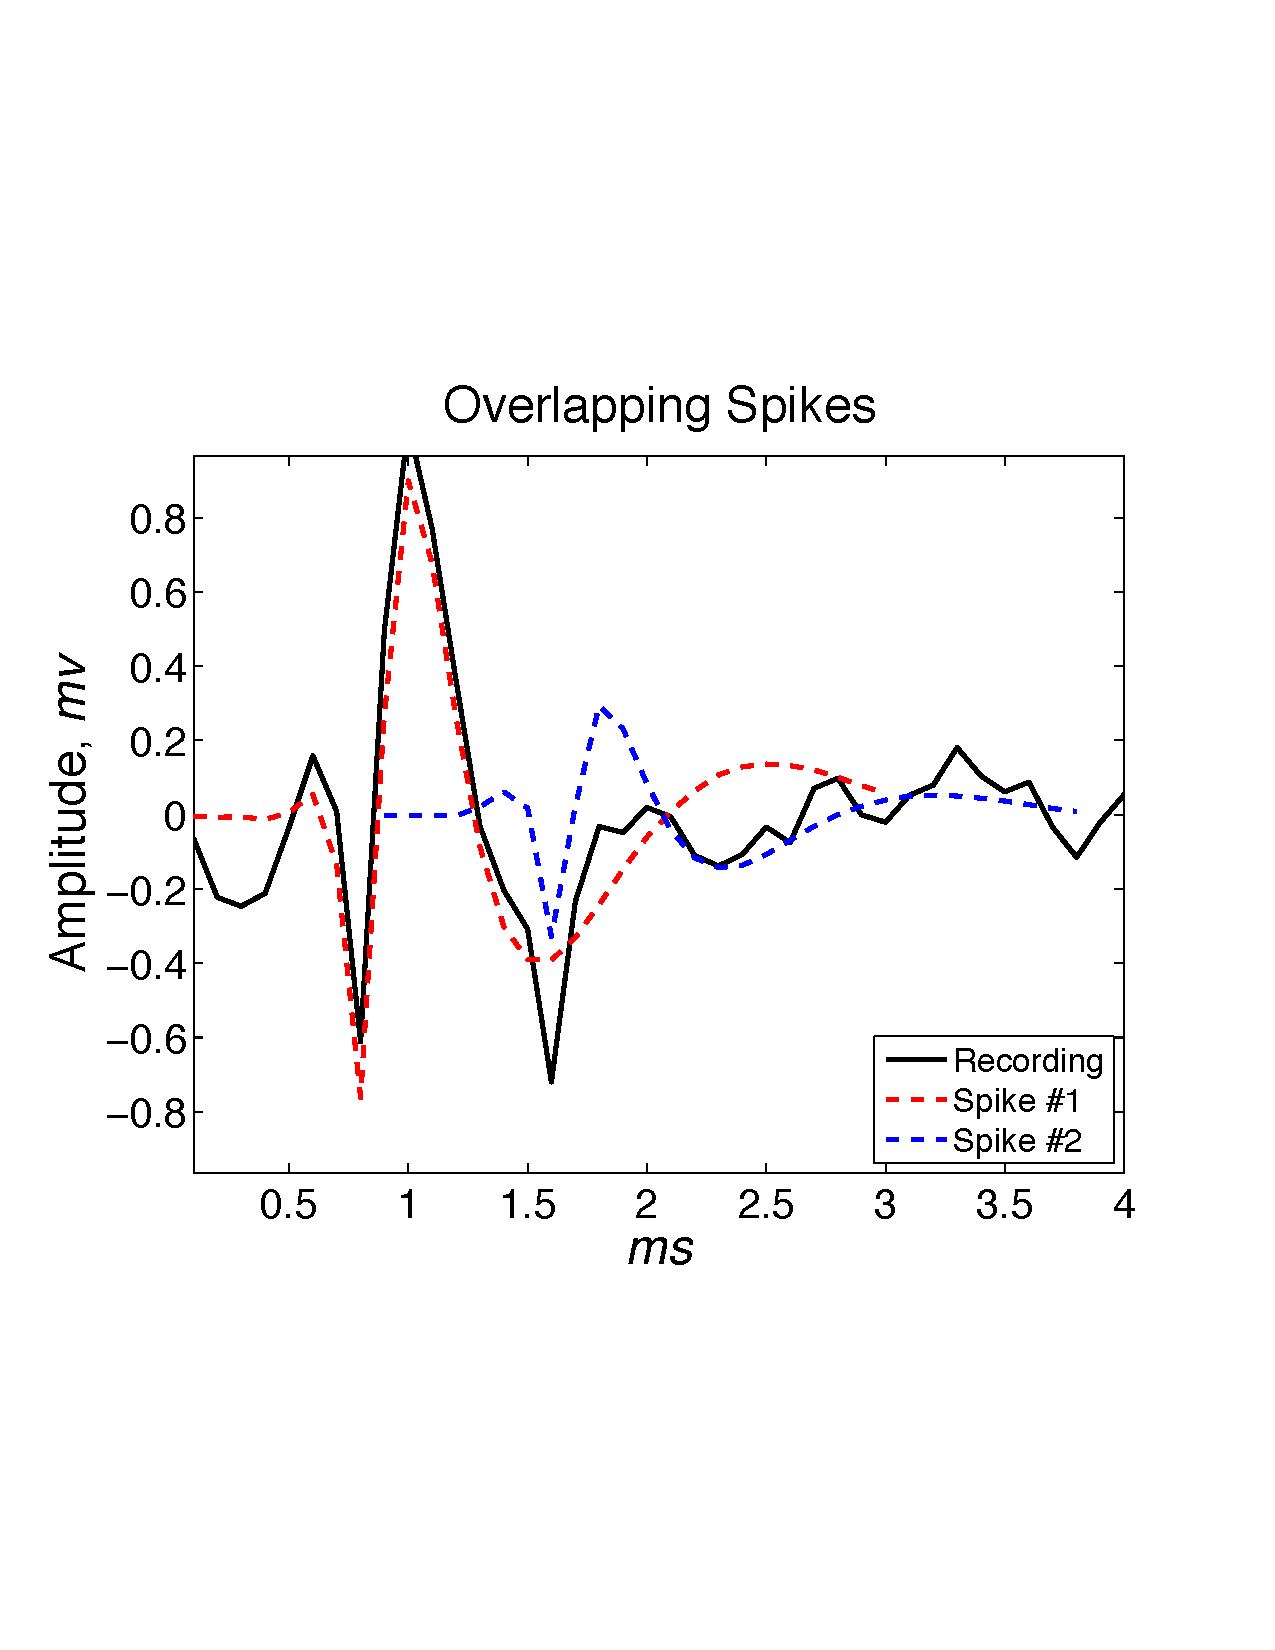
\includegraphics[width=\textwidth]{../figs/alloverlappingspikes/olspike3}
\caption{}
\label{fig:overlapping}
\end{subfigure}
\begin{subfigure}[b]{.3\textwidth}
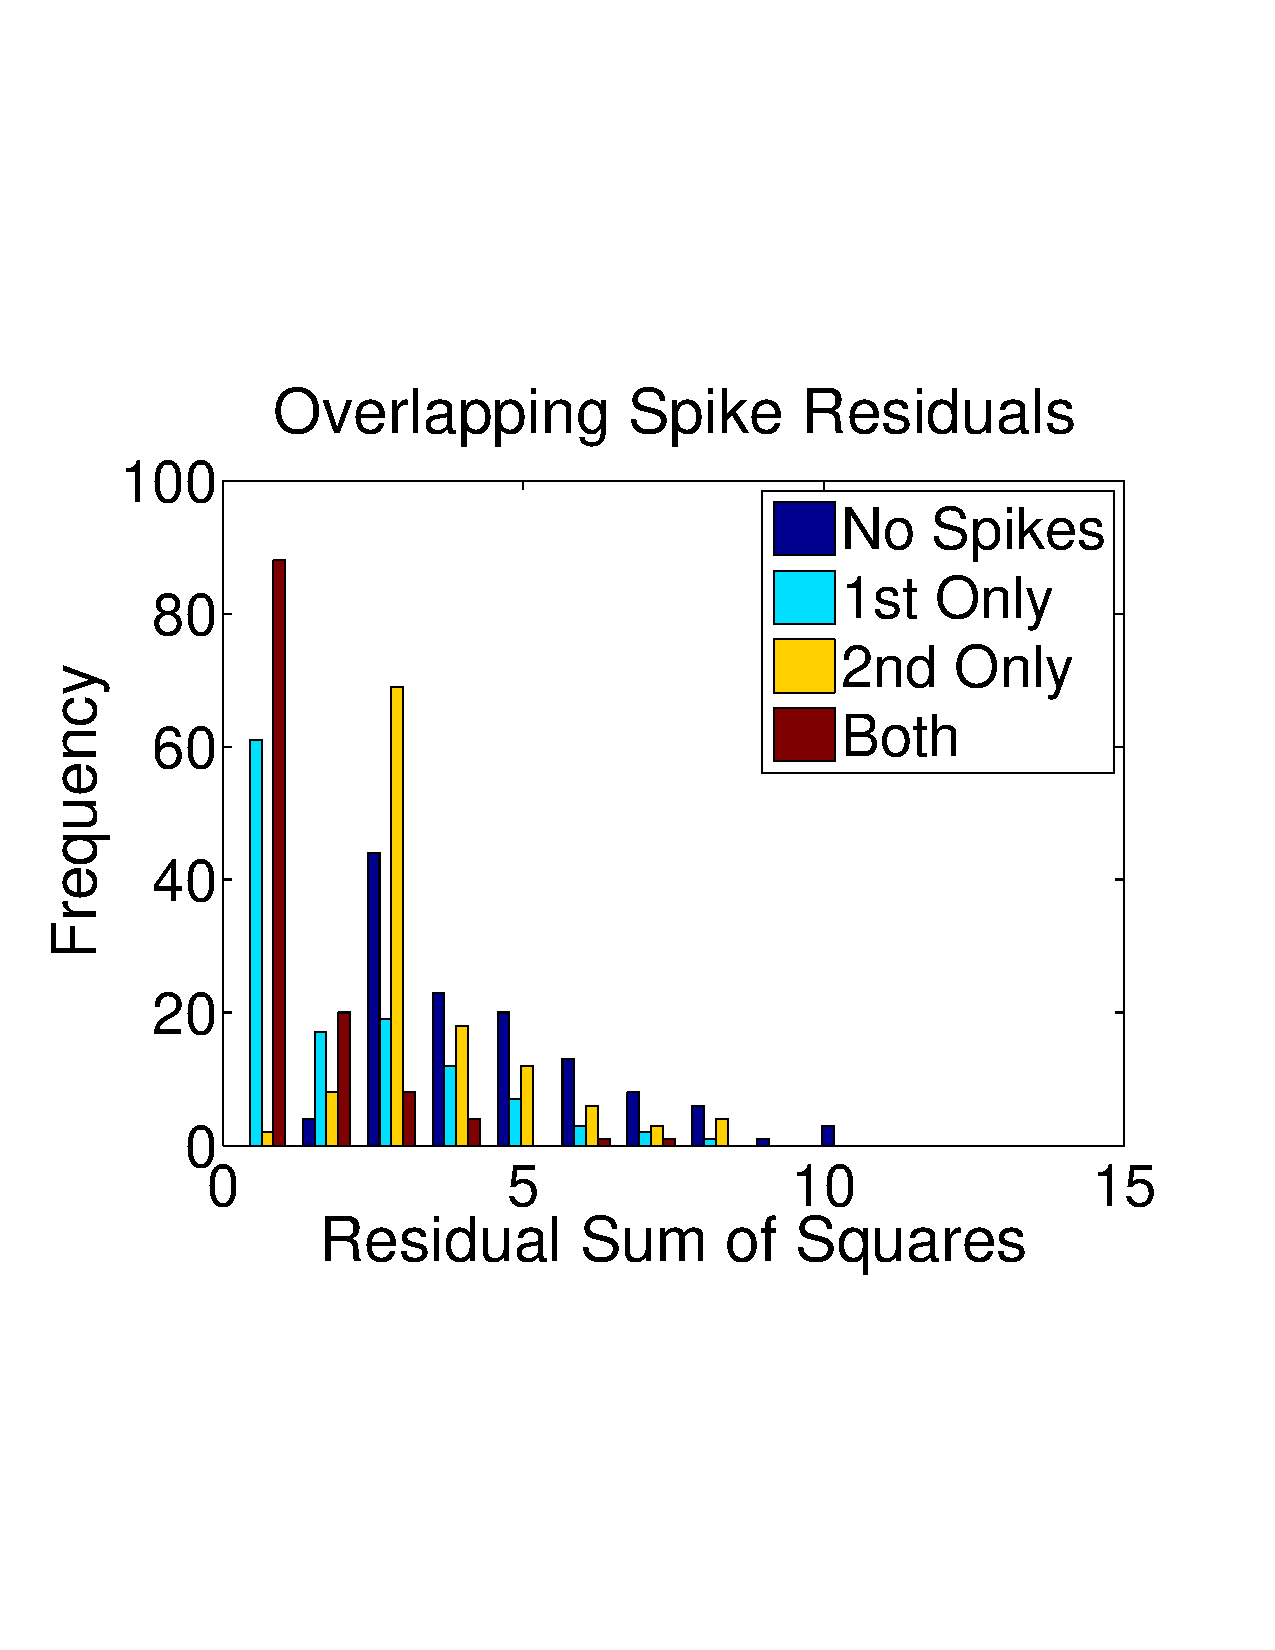
\includegraphics[width=\textwidth]{../figs/overlappingstat.pdf}
\caption{}
\label{fig:resid}
\end{subfigure}
\caption{Results on the d533101 dataset.  (a) \jovo{like this but also with the sum} (b) \jovo{residuals for this example.} (c) \jovo{histogram of residuals for all putative overlapping examples. keep colors consistent across all three panels.  i think line plots for the histograms would more clearly indicate that residuals are significantly smaller than the others.}}
\end{SCfigure}
\end{center}



\subsection{Time-Varying Waveform Adaptation} \label{sub:adapt}


As as been demonstrated previously \cite{calabrese2011kalman}, the waveform shape of a neuron may change over time.  The mean waveform over time for the intracellular neuron is shown in Figure \ref{evohc1}.  Clearly, the mean waveform is changing over time.  Moreover, these changes are reflected in the principal component space (see Figure \ref{fig:clusterevo}).  We therefore compared means and variances \smug\ with \smug\sct{R} which models the mean of the dictionary weights via an auto-regressive process.  Figure \ref{fig:AR} shows that the auto-regressive model for the mean dictionary weights yields a time-varying posterior (top), whereas the static prior yields a constant posterior mean with increasing posterior marginal variances (bottom).  Indeed, the \smug\sct{R} yields 11 more true detections than \smug.
 


\begin{center}
\begin{figure}
\begin{subfigure}[b]{.33\textwidth}
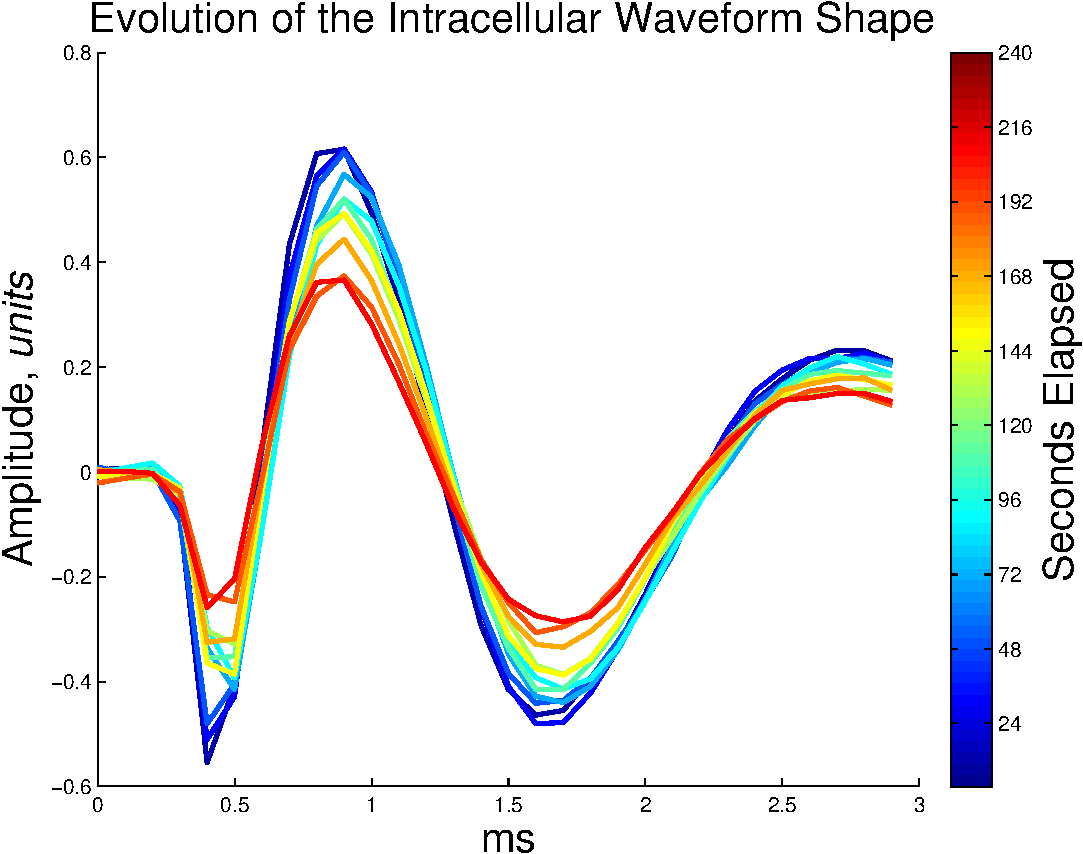
\includegraphics[width=\textwidth]{../figs/evohc1}
\caption{}
\label{evohc1}
\end{subfigure}
\begin{subfigure}[b]{.33\textwidth}
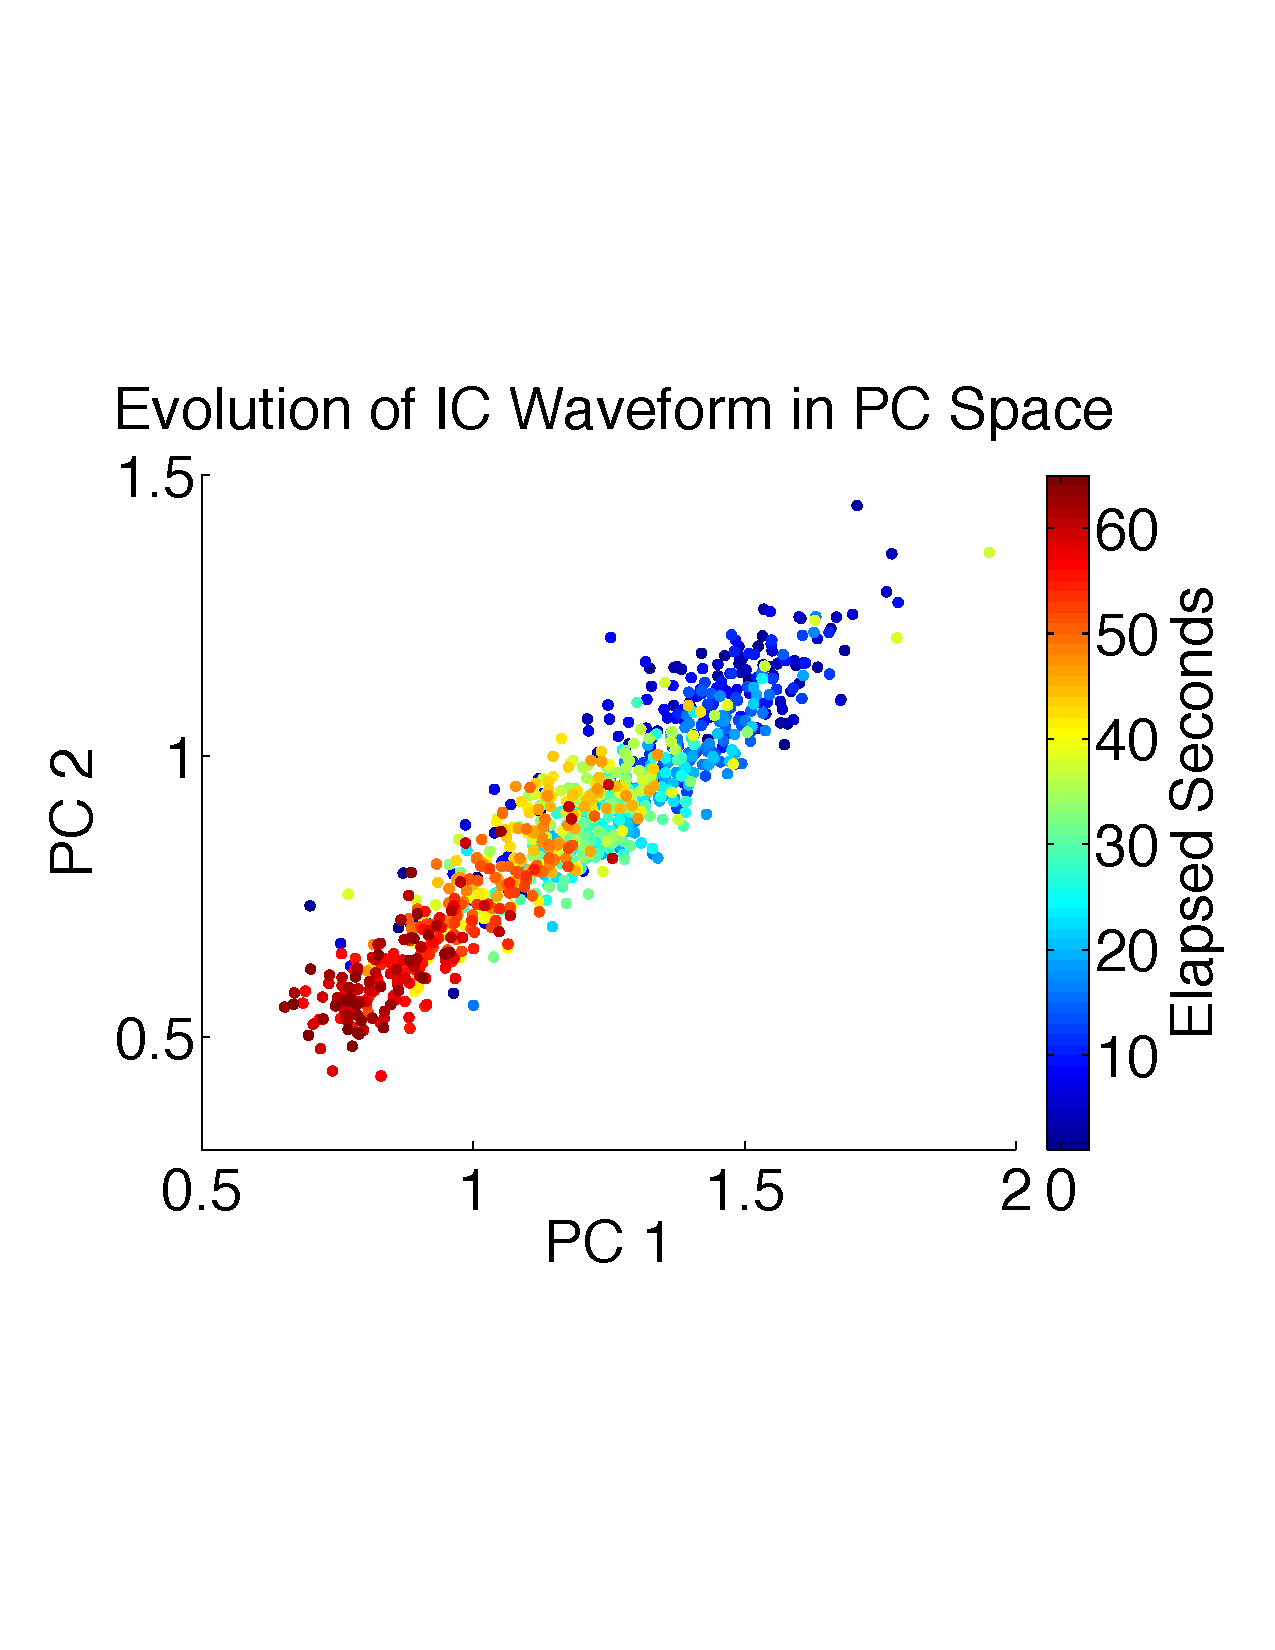
\includegraphics[width=\textwidth]{../figs/new/clusterevo.pdf}
\caption{}
\label{fig:clusterevo}
\end{subfigure}
\begin{subfigure}[b]{.33\textwidth}
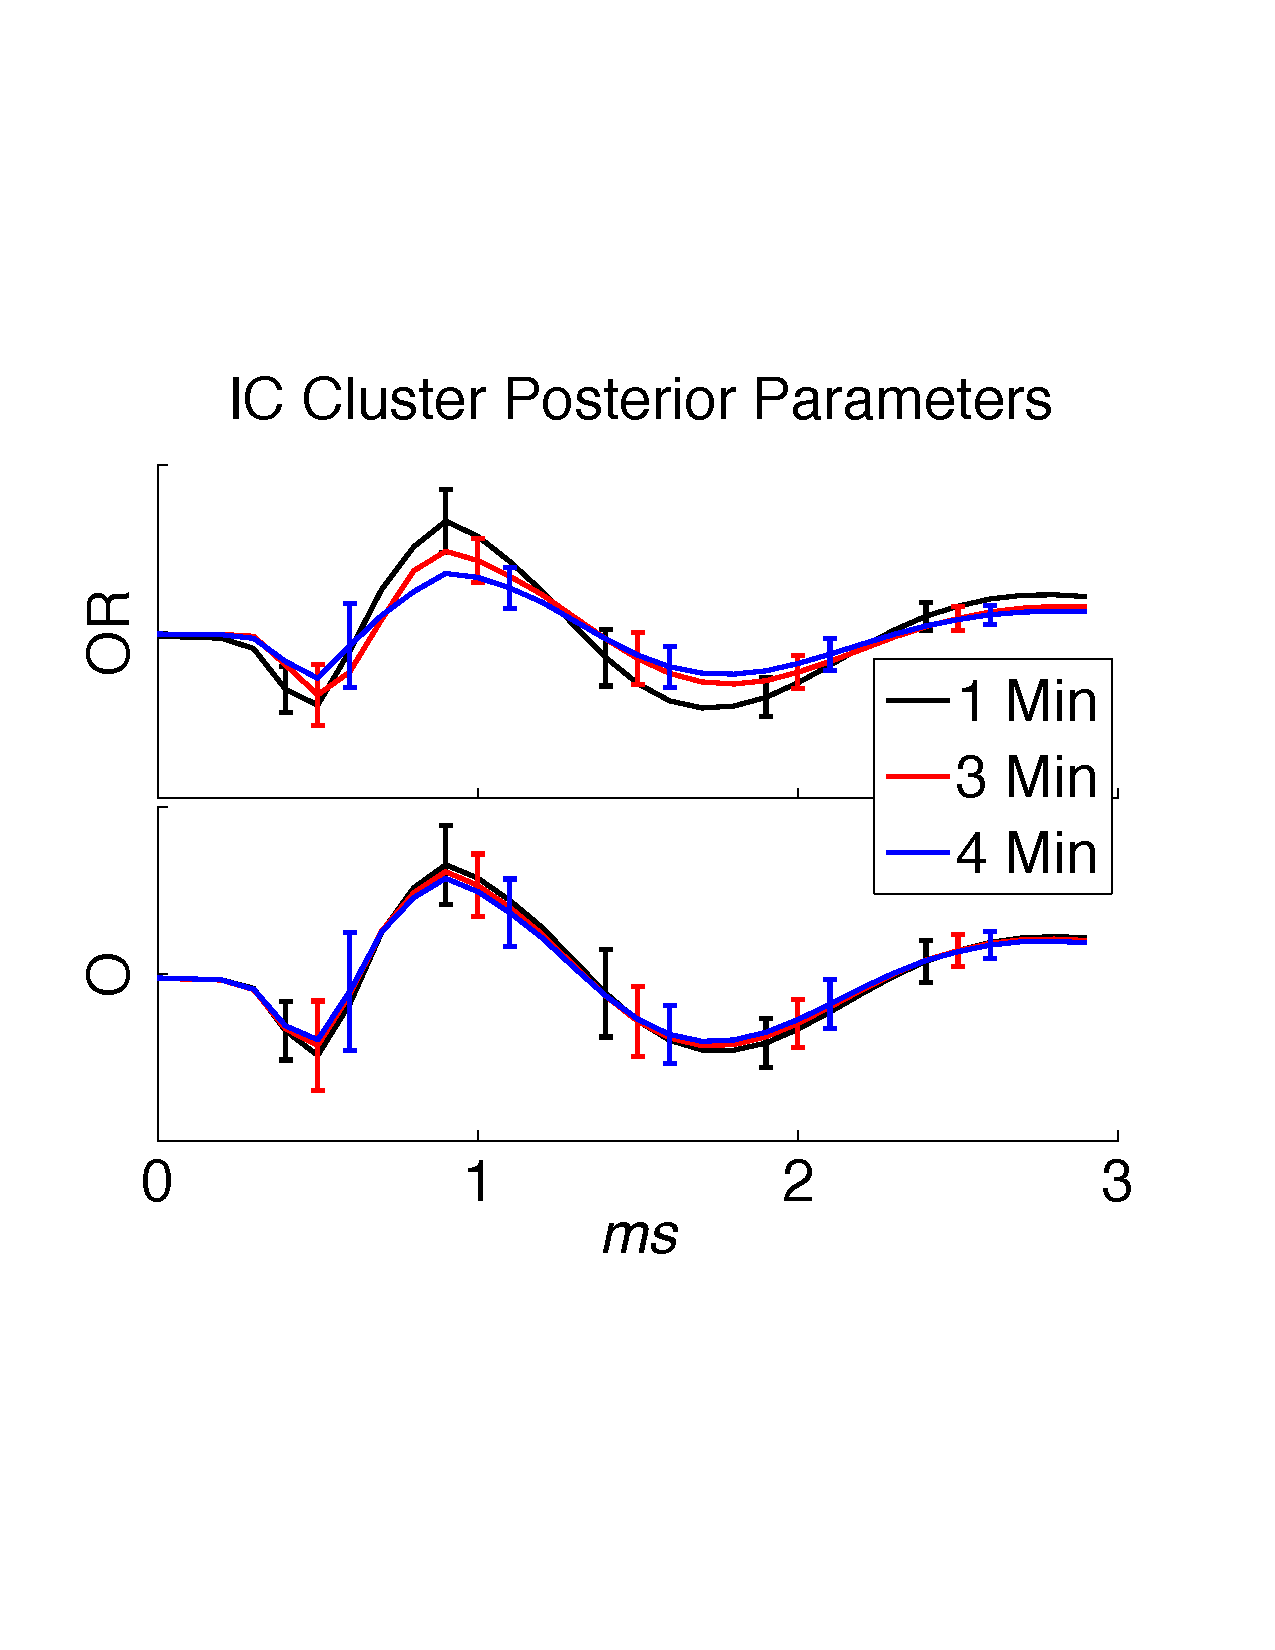
\includegraphics[width=\textwidth]{../figs/new/ARvsStationary.pdf}
\caption{}
\label{fig:AR}
\end{subfigure}
\caption{
(a) Mean IC waveforms over time.  Each colored line represents the mean of the waveform averaged over 24s and the color gives the elapsed time.  This neuron decreases in amplitude over the period of the recording. 
(b) \jovo{take out scale bars.}
(c) \jovo{plot 3 ARs on top of each other, and also plot 3 stationary on top of each other.}
\jovo{AR: mean 0.0037  std  0.0038
   other: mean 0.0077  std  0.0071}
}
\end{figure}
\end{center}

\subsection{Multi-Electrode Array} \label{sub:multi}

\jovo{add grids to all panels of all figs by default, remove if it looks shitty.}


In the tetrode case the waveform undoubtedly appears on all channels at once; it is possible to concatenate the channels to jointly process the data \cite{wood2009}.  When the action potential will only appear on a subset of channels it is nice to allow the action potential to vary in a low-dimensional subset in each of the channels instead of a low-dimensional subset over all the channels. \cite{Prentice2011}

We use processed data from novel NeuroNexus devices implanted in the rat motor cortex.  The data was recorded at 32.5kHz in freely-moving rats, and the data was first processed by high-pass filtering at 800Hz.  The first device we consider is a set of 3 channels of data shown in Figure \ref{3dev}.  The neighboring electrode sites in these devices have 30 $\mu$m between electrode edges and 60 $\mu$m between electrode centers.  These devices are close enough that a locally-firing neuron could appear on multiple electrode sites (cite that paper on action potential overlap), and neighboring channels warrant joint processing.  The second, 8-channel device is shown in Figure \ref{8dev}, and has similar properties to the first device.

 The top 2 clusters found in the first 10 minutes of data on the 3-channel device are shown in Figures \ref{ex31}, \ref{ex32}.  The waveform in channel 3 is very similar for the waveforms in Figure \ref{ex31} and \ref{ex32}, and would be difficult to separate if we were analyzing each channel individually; the representation of those two clusters in PCA space on channel 3 is shown in Figure \ref{chpca}.  We gain the ability to distinguish the waveforms by looking at all the channels simultaneously.  The top 3 clusters found in the 8-channel device can be found in Figures \ref{ex81}, \ref{ex82}, and \ref{ex83}.

{\color{red} perhaps add comments about time-evolution and the false positives we avoid by using multi-channel analysis}


\begin{center}
\begin{figure}
\begin{subfigure}[b]{.12\textwidth}
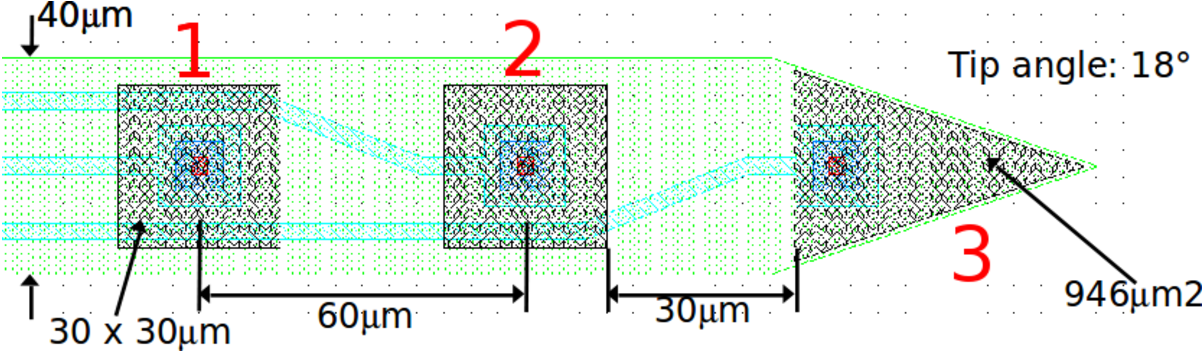
\includegraphics[width=1\textwidth]{../figs/3dev}
\caption{}
\label{3dev}
\end{subfigure}
\begin{subfigure}[b]{.28\textwidth}
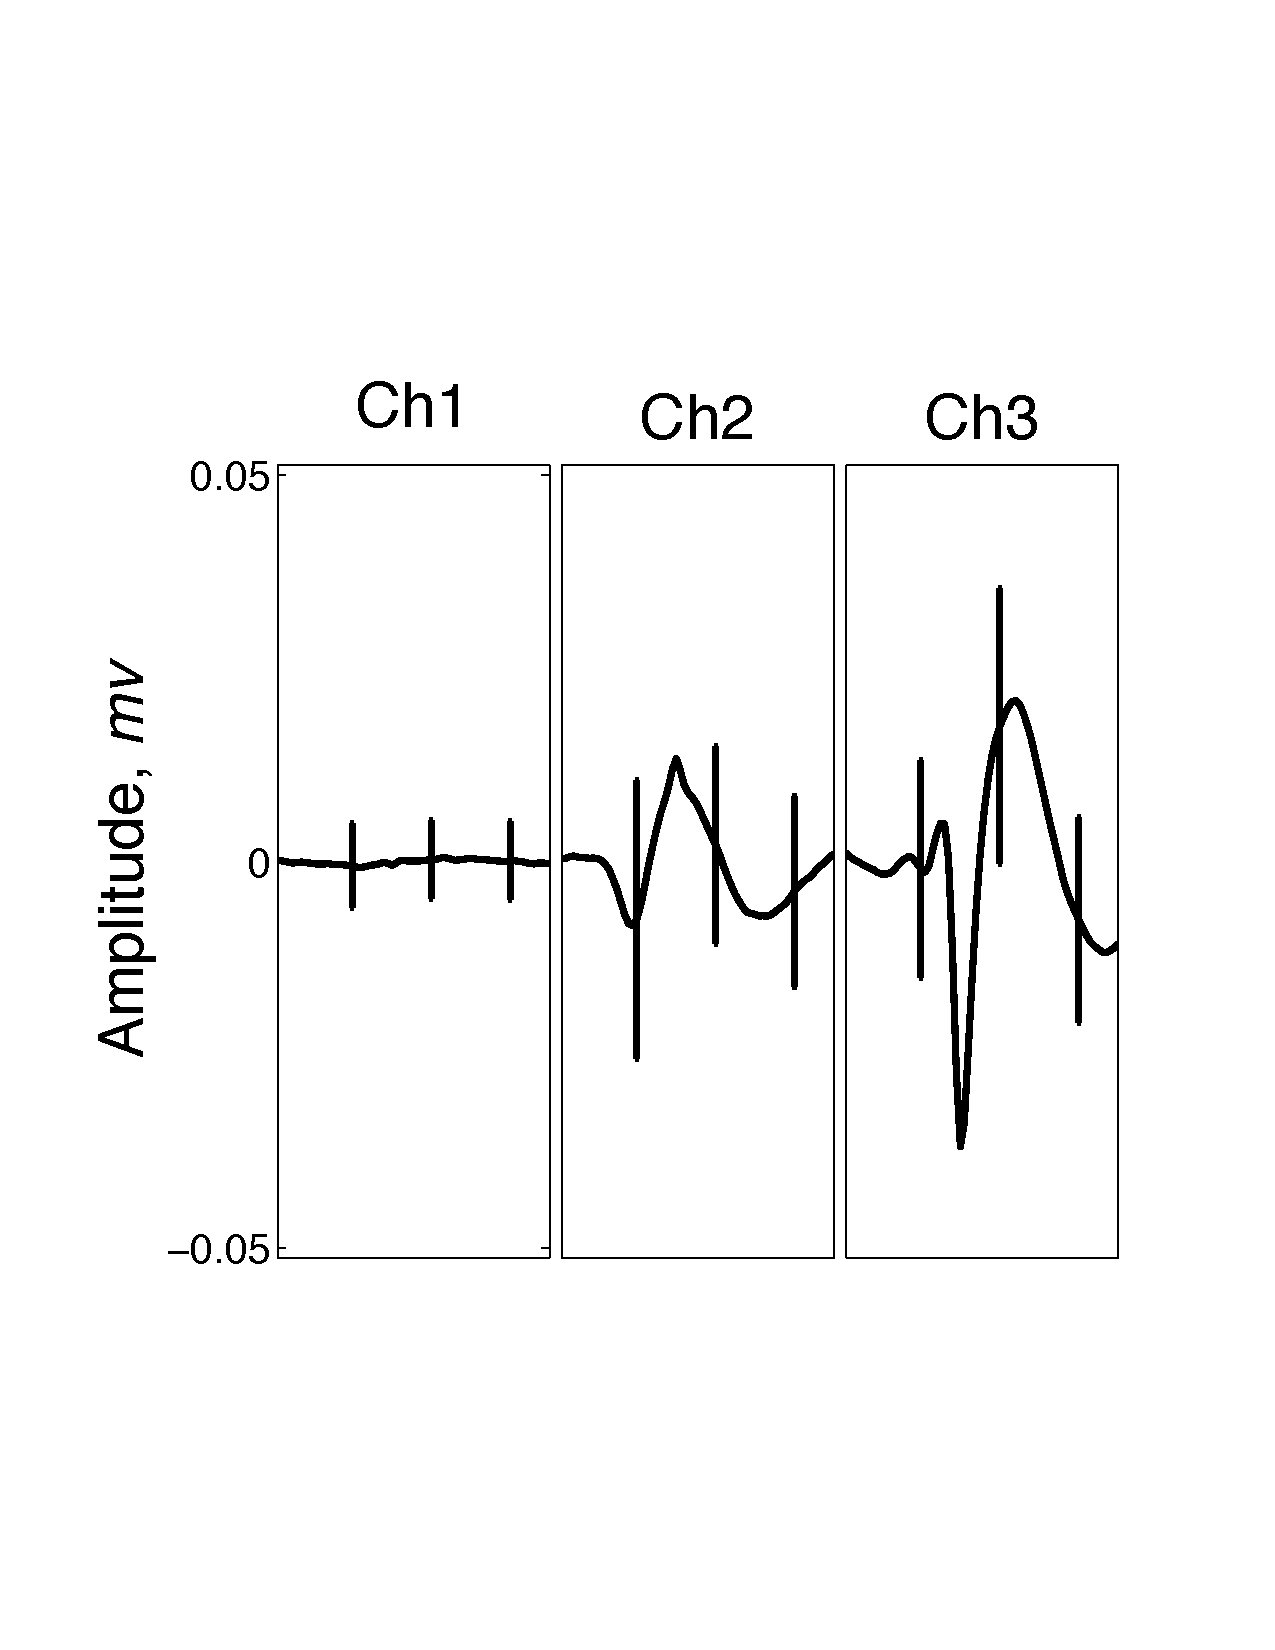
\includegraphics[width=\textwidth]{../figs/3devim/clus1}
\caption{}
\label{ex31}
\end{subfigure}
\begin{subfigure}[b]{.28\textwidth}
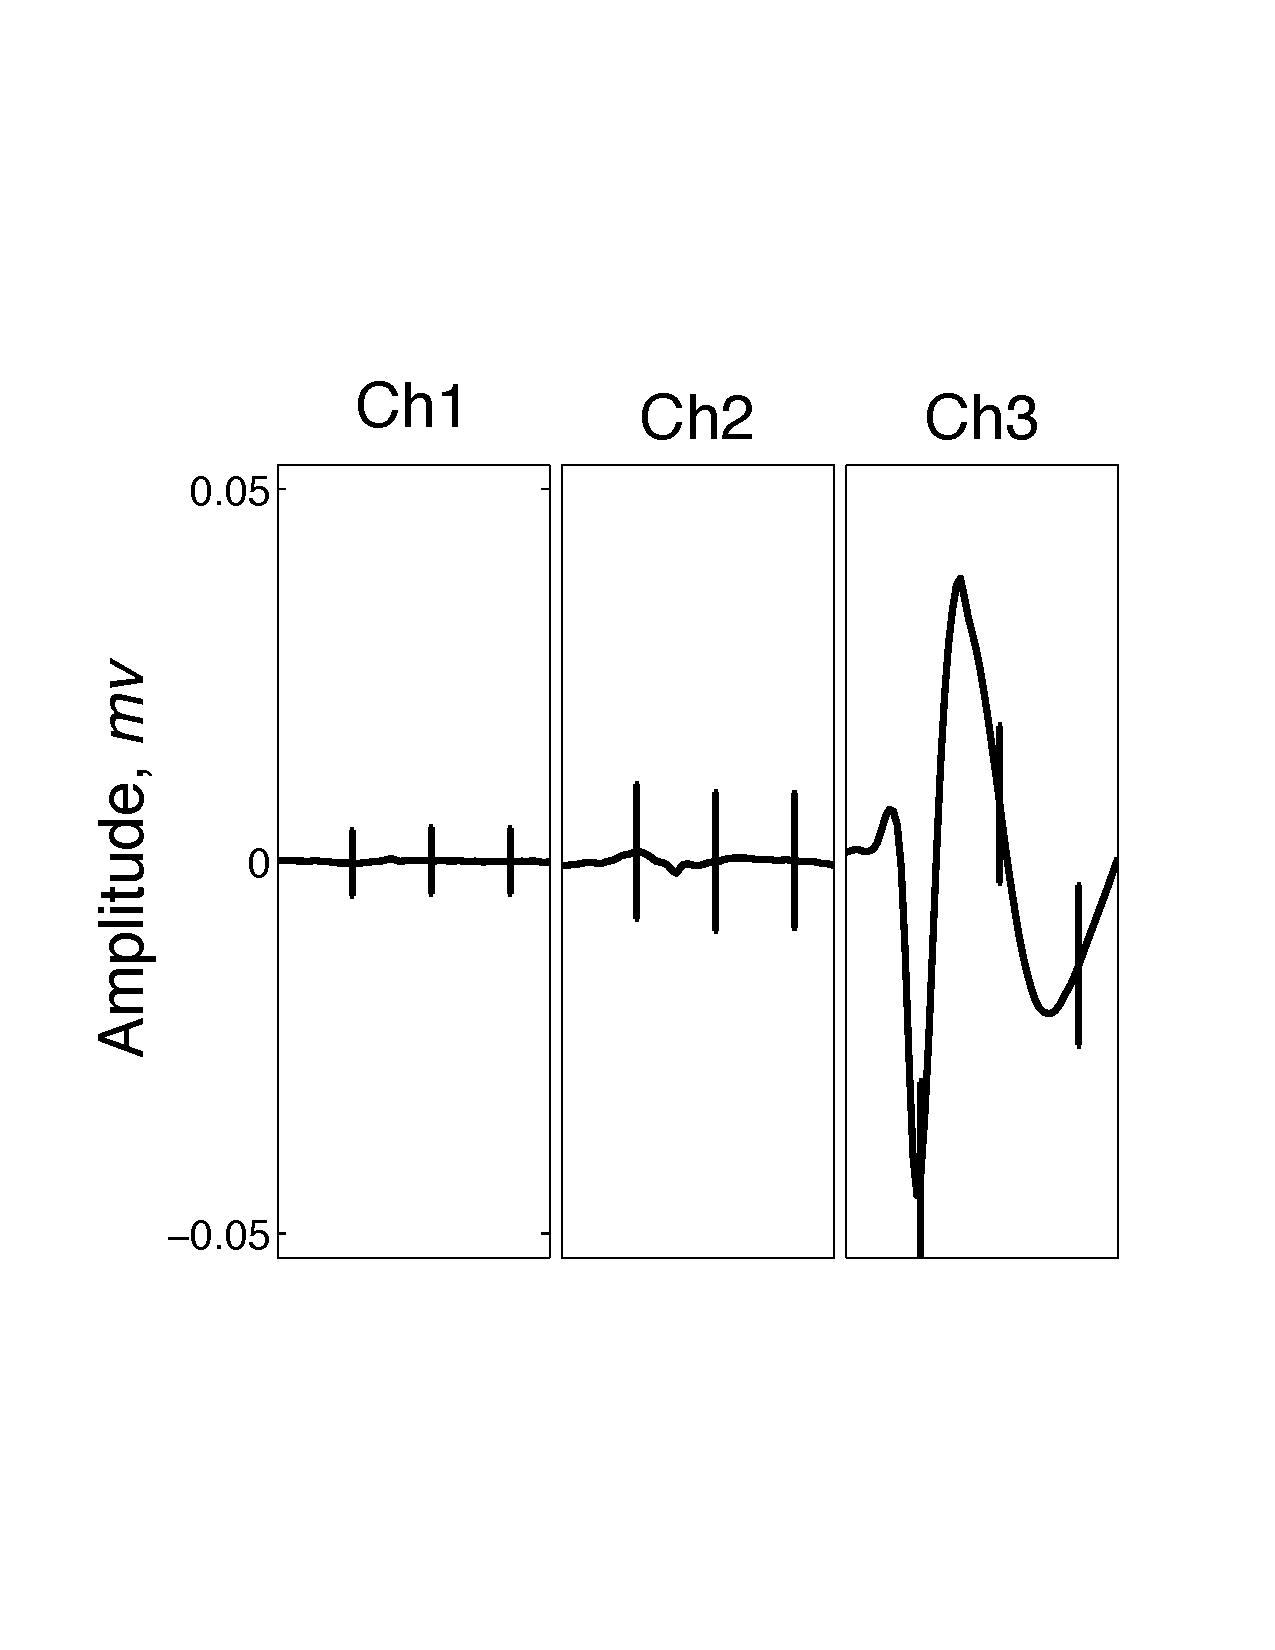
\includegraphics[width=\textwidth]{../figs/3devim/clus2}
\caption{}
\label{ex32}
\end{subfigure}
\begin{subfigure}[b]{.28\textwidth}
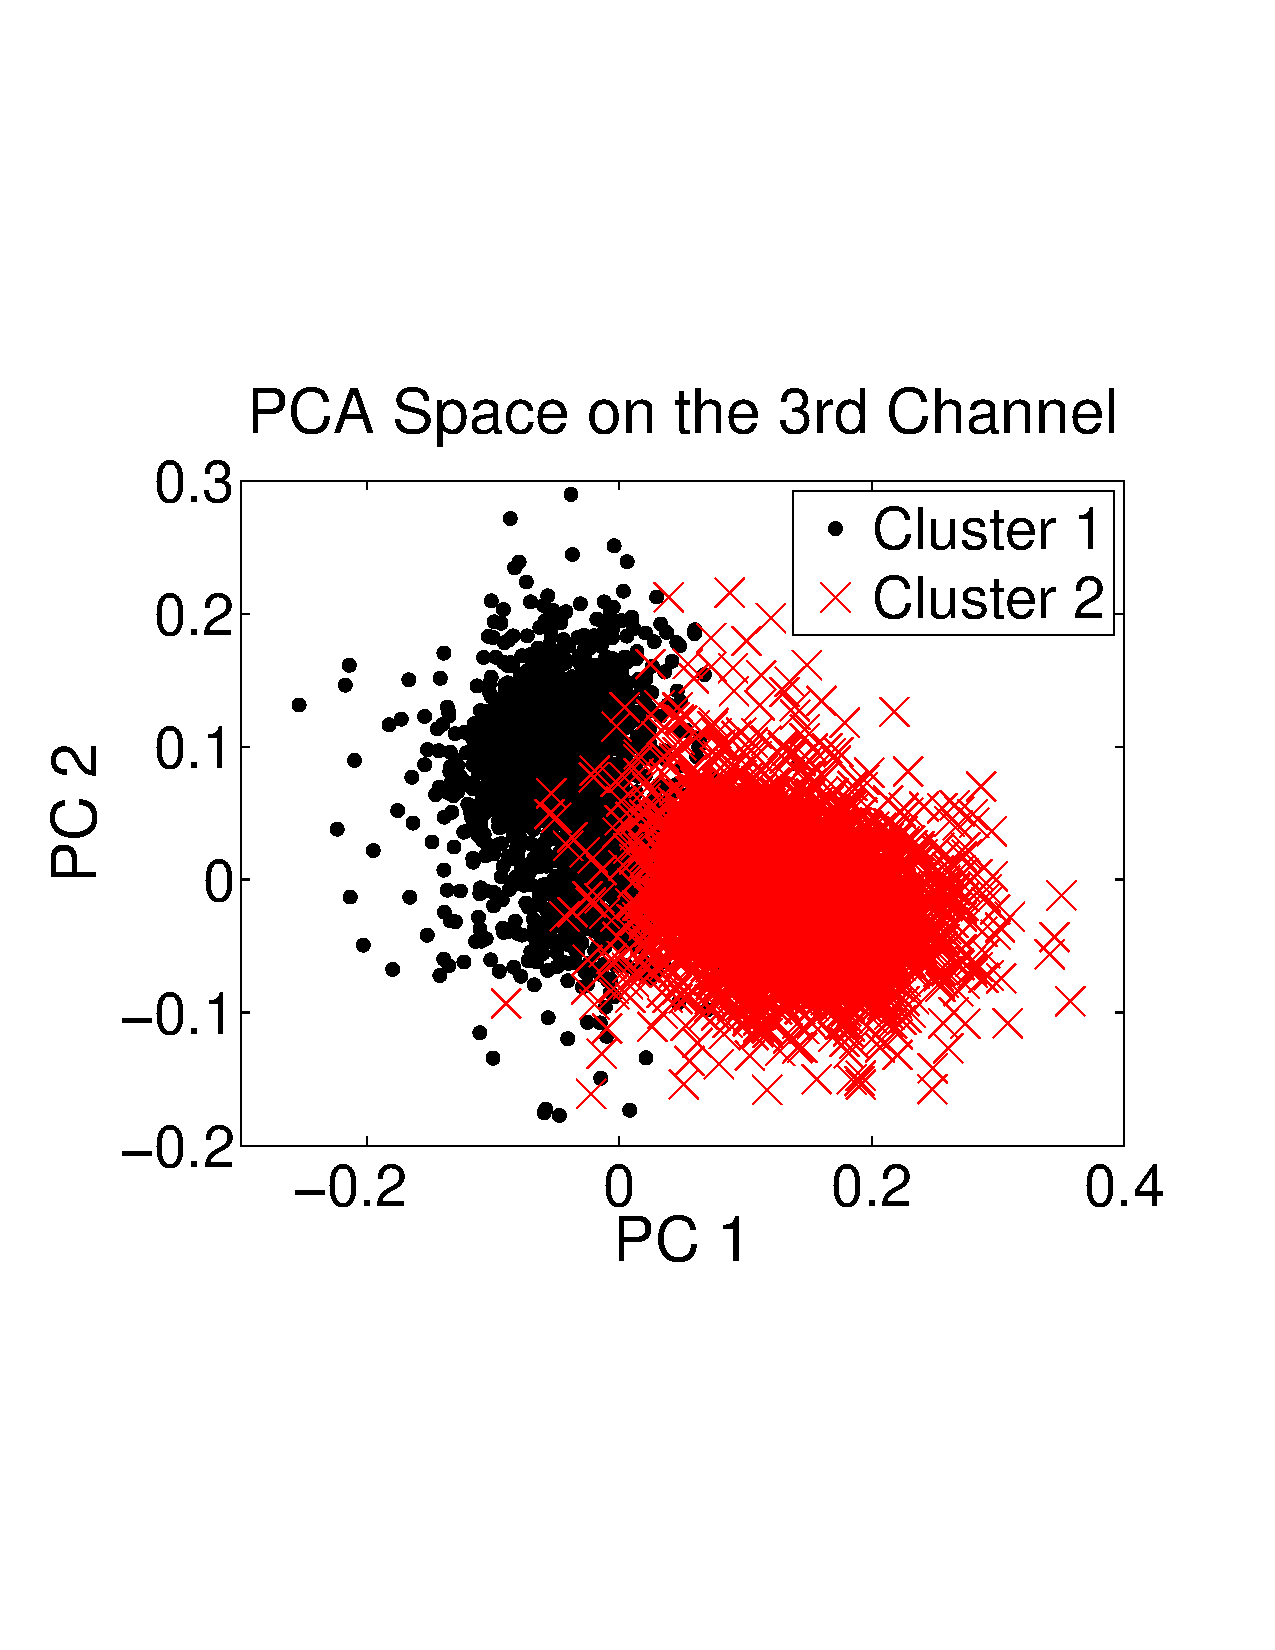
\includegraphics[width=\textwidth]{../figs/new/3chpca}
\caption{}
\label{3chpca}
\end{subfigure}
% \caption{}
% \end{figure}
% \end{center}
% \begin{center}
% \begin{figure}[h!]
\begin{subfigure}[b]{.12\textwidth}
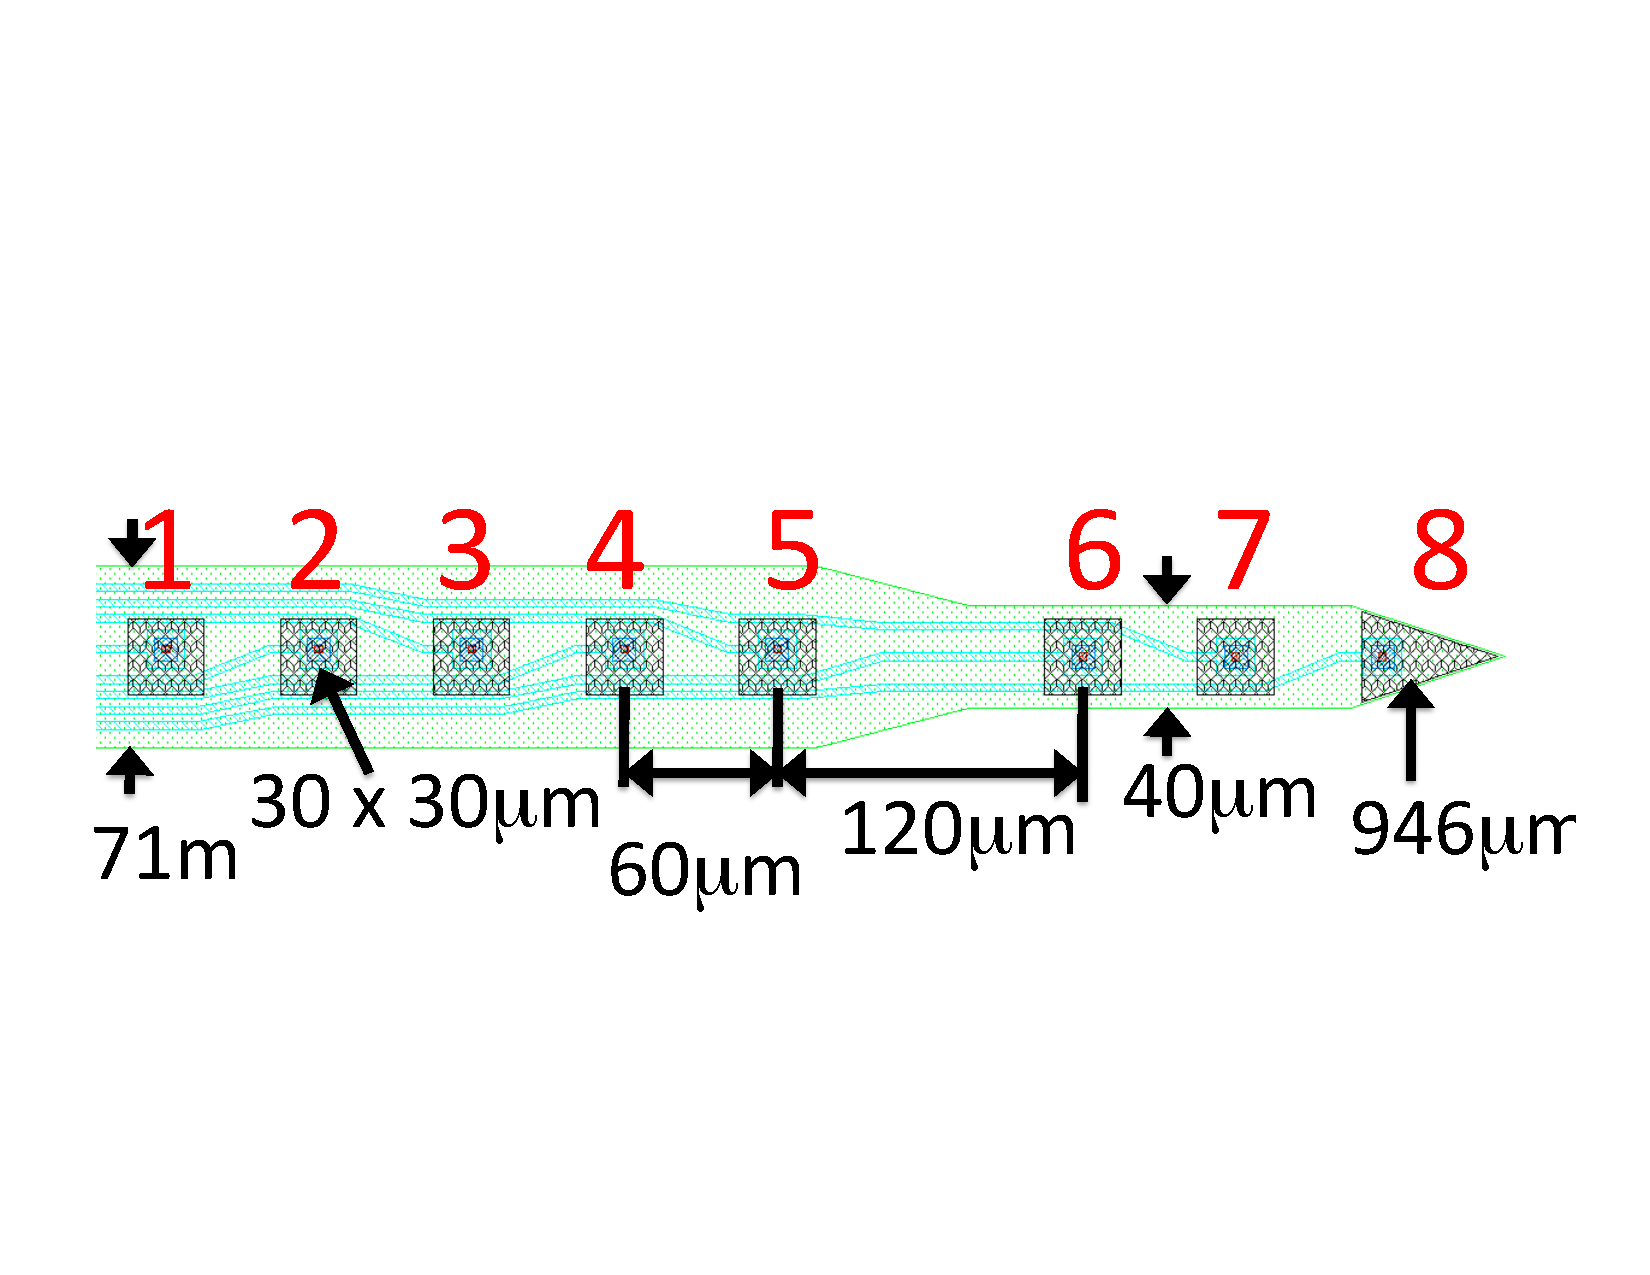
\includegraphics[width=0.8\textwidth]{../figs/8dev}
\caption{}
\label{3dev}
\end{subfigure}
\begin{subfigure}[b]{.28\textwidth}
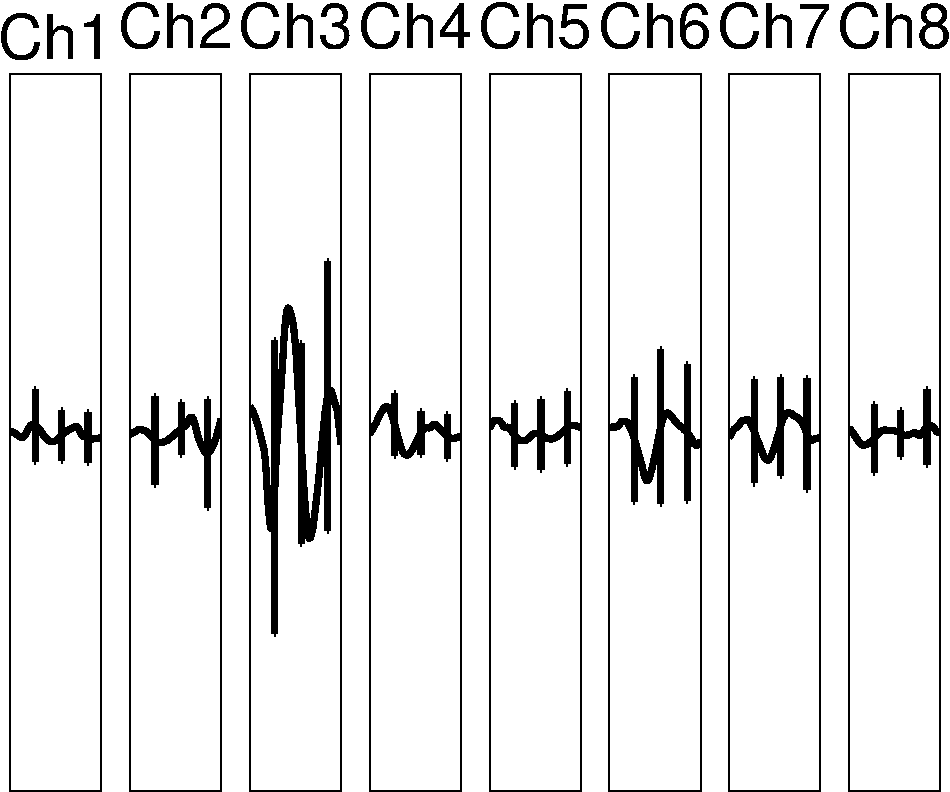
\includegraphics[width=\textwidth]{../figs/8devim/clus3}
\caption{}
\label{ex81}
\end{subfigure}
\begin{subfigure}[b]{.28\textwidth}
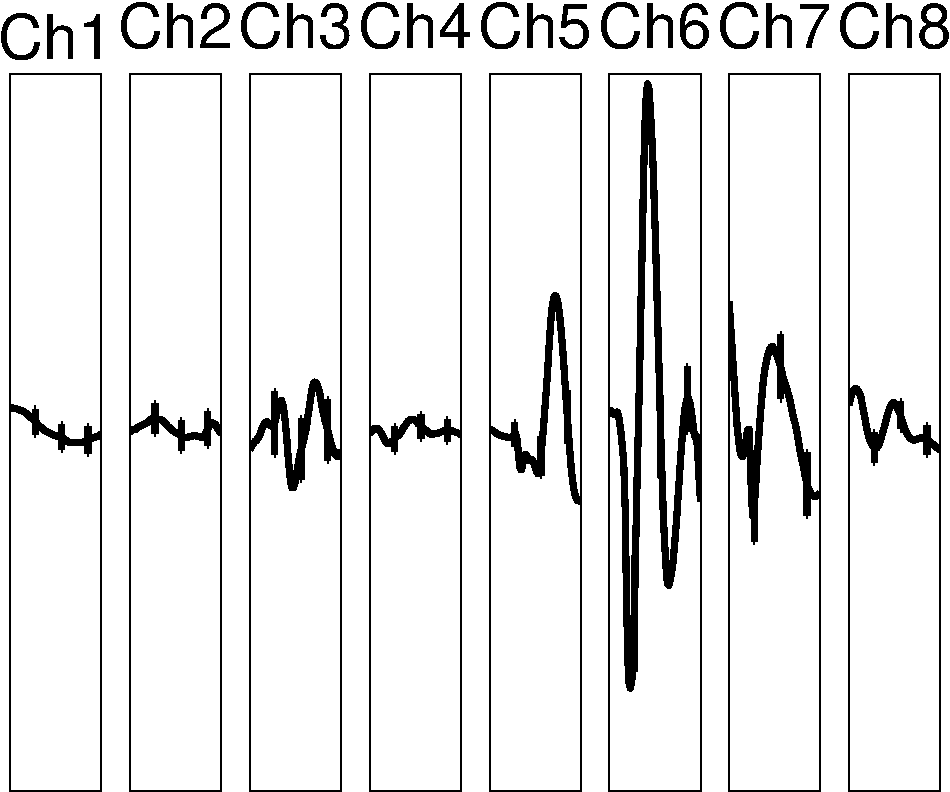
\includegraphics[width=\textwidth]{../figs/8devim/clus9}
\caption{}
\label{ex82}
\end{subfigure}
\begin{subfigure}[b]{.28\textwidth}
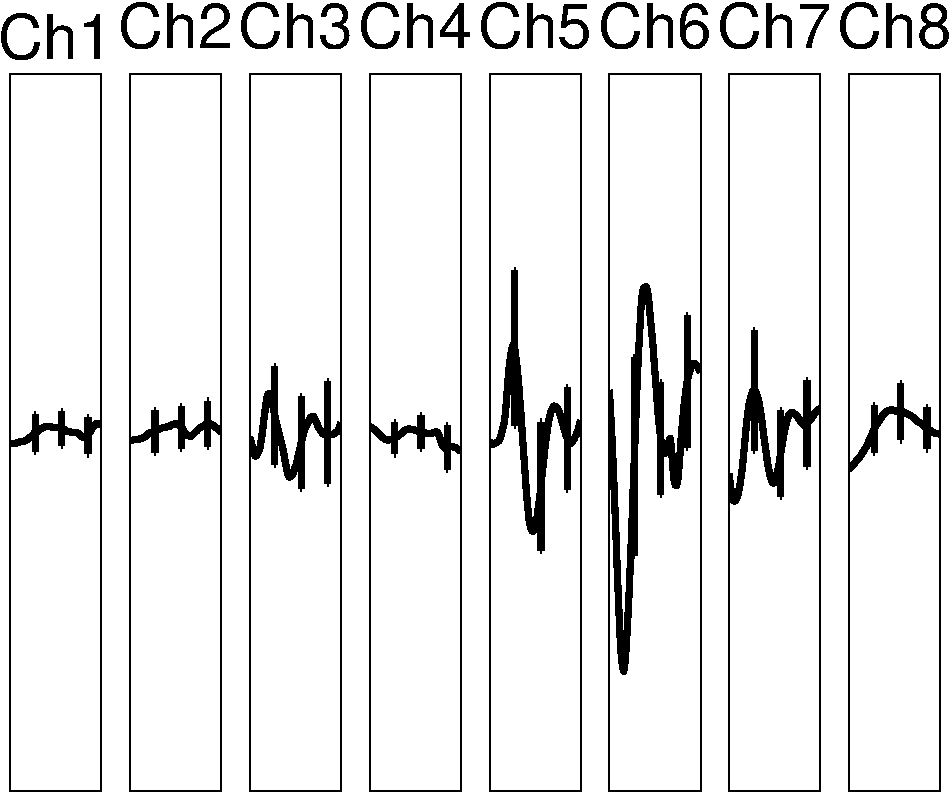
\includegraphics[width=\textwidth]{../figs/8devim/clus6}
\caption{}
\label{ex83}
\end{subfigure}
\caption{
(a) Three electrode device showing local proximity of electrodes with channel indexes in large, red numbers. (b,c) Top 2 most prevalent waveforms.  Each waveform shape is 2ms long.   Note in (a) we have a waveform that appears on both channel 2 and channel 3, whereas in (b) the waveform only appears in channel 3.  If only channel 3 was used, it would be difficult to separate the waveform in (a) and (b), as is demonstrated in Figure (d) by the representation of detected spikes on the 3rd channel in PCA space.
(e)8 electrode device showing local proximity of electrodes with channel indexes in large, red numbers. (f,g,h) Top 3 most prevalent waveforms.  Each waveform shape is 2ms long.
\jovo{update these in various ways that you know.}
}
\end{figure}
\end{center}




\subsection{Limitations of Dictionary-Based Techniques} \label{sub:template}



\begin{center}
\begin{figure}[h!]
\begin{subfigure}[b]{.33\textwidth}
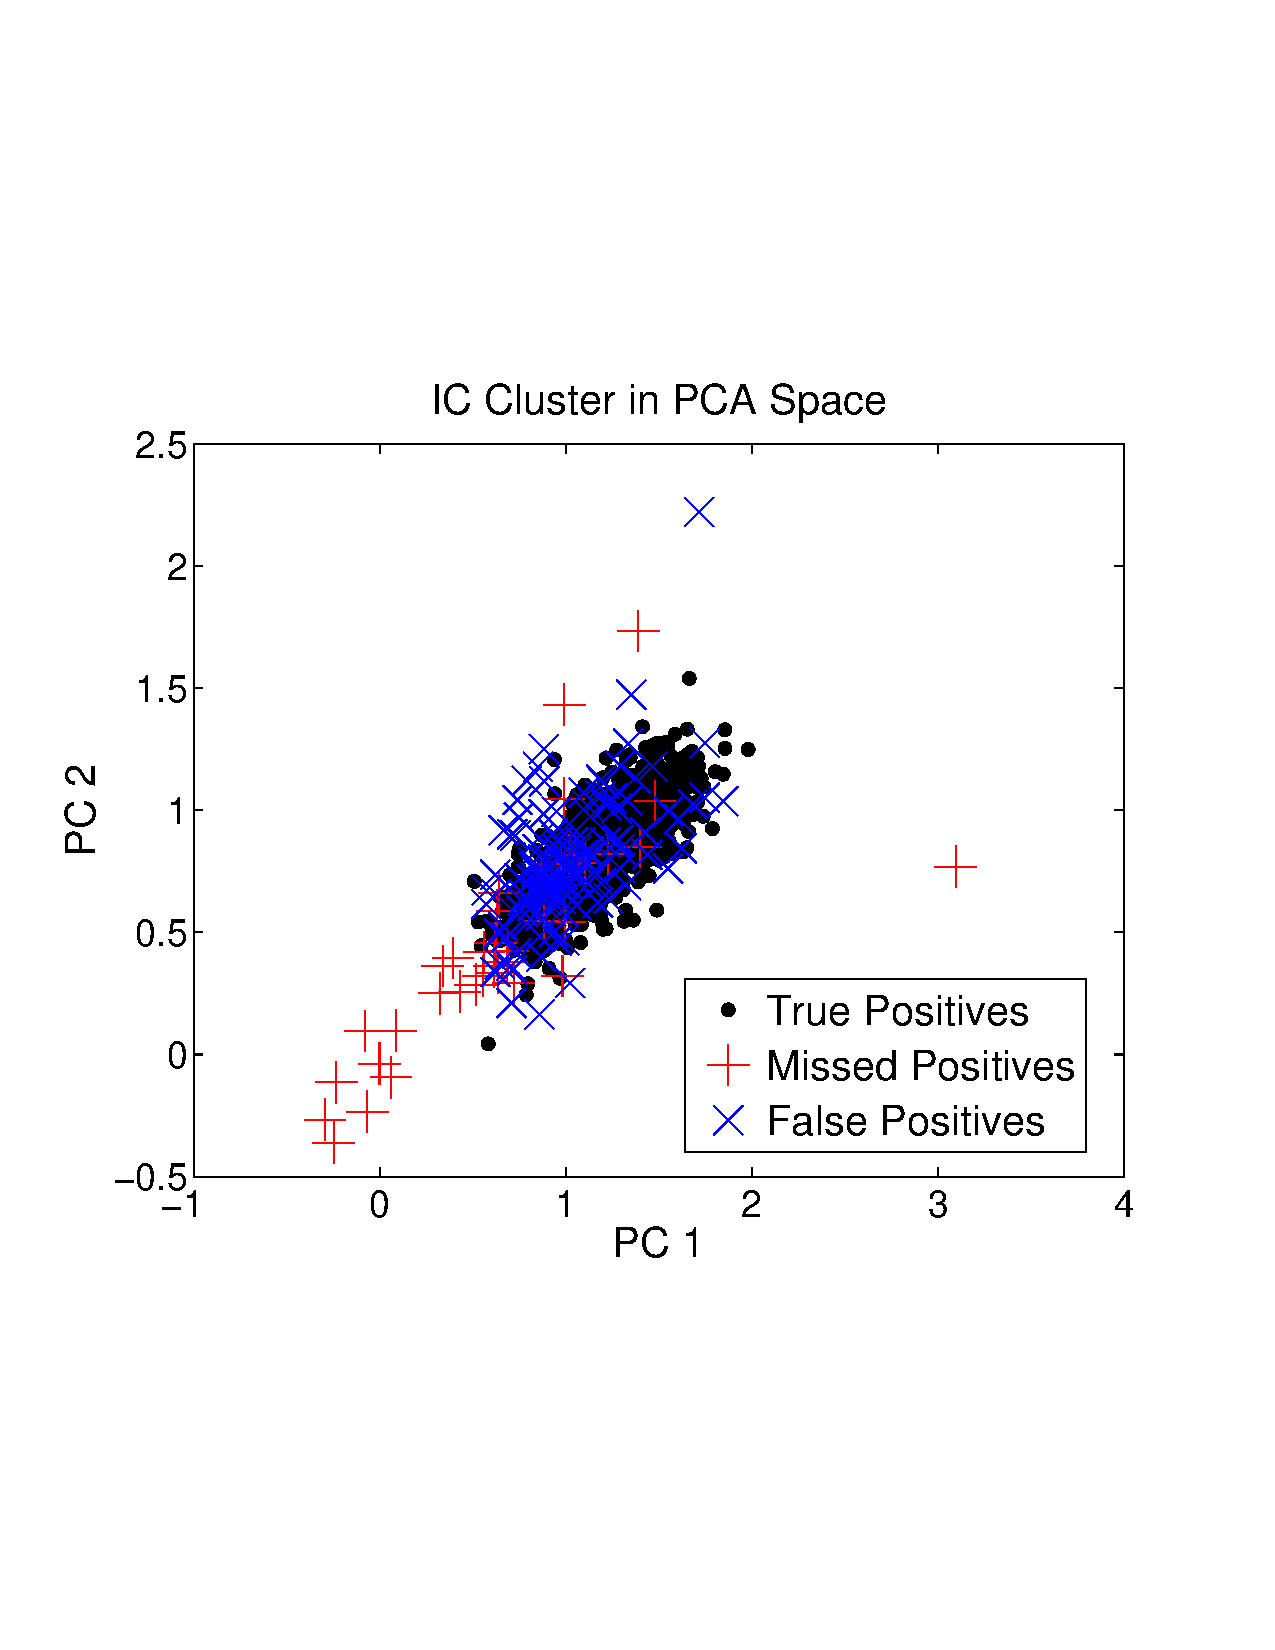
\includegraphics[width=\textwidth]{../figs/new/ICclusteroldpca.pdf}
\caption{}
\label{fig:ICold}
\end{subfigure}
\begin{subfigure}[b]{.33\textwidth}
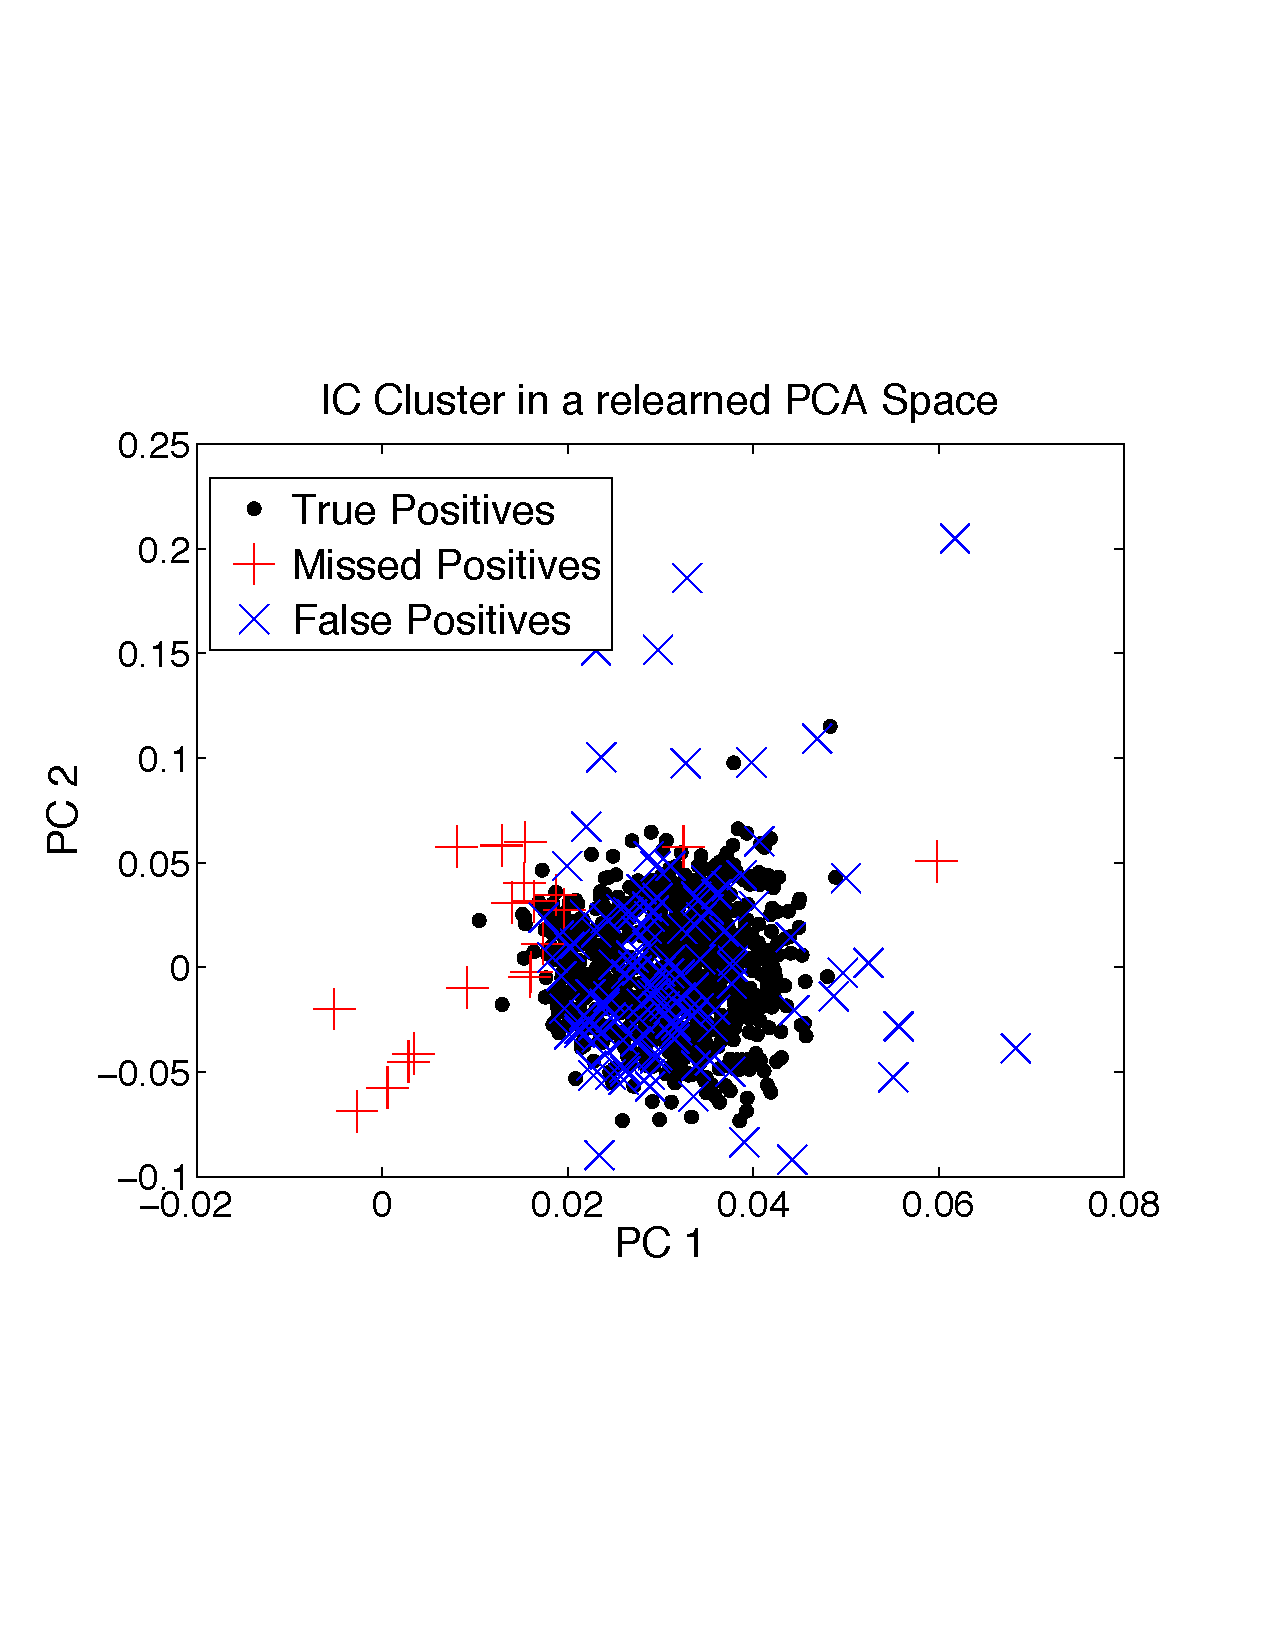
\includegraphics[width=\textwidth]{../figs/new/ICclusternewpca.pdf}
\caption{}
\label{fig:ICnew}
\end{subfigure}
\begin{subfigure}[b]{.33\textwidth}
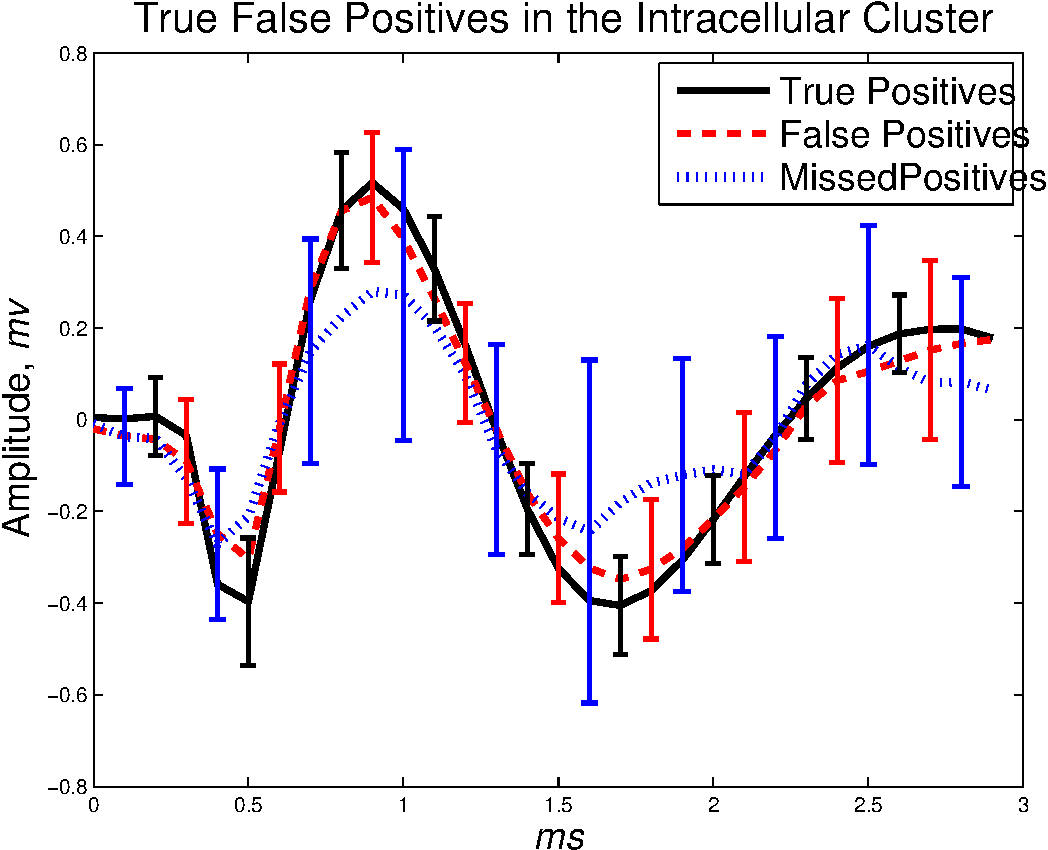
\includegraphics[width=\textwidth]{../figs/IntracellularTrueFalsePositivesv2}
\caption{}
\label{truewaveforms}
\end{subfigure}
\caption{Template matching.
(c) Errorbar plots of the true positives and the false positives in the IC cluster.  While the false positives have slightly more variability, the mean shape for the false positives and the true positives is nearly identical.  The true misses have a significantly lower amplitude as well as high variability. 
} \label{fig:IC-PCA}
\end{figure}
\end{center}



















 
\section{Discussion}
% \paragraph{Summary}

We have developed a novel Bayesian nonparametric model for spike sorting, and a novel faster than real-time  inference algorithm called \smug.  
%Our model and inference procedure incorporate certain features that previous approaches---be they nonparametric or not---lacked.  
%Most importantly, we developed a variational Bayesian online inference scheme, that enabled faster than real-time posterior inference.  
%Such computational efficiency is crucial for sequential experimental design \cite{}.  
Although we only provided our algorithm with streaming data, our fully Bayesian model \smug\ outperformed all competitor \emph{batch} algorithms 
%(that is, algorithms that consume all the data at once). 
Our improved sensitivity and specificity seem to arise from multiple sources including (i) improved detection, (ii) accounting for correlated noise, 
(iii) capturing overlapping spikes, (iv) tracking waveform dynamics, and (v) utilizing multiple channels.  
While others have developed closely related Bayesian models for clustering \cite{WoodBla2008,wood2009}, deconvolution based techniques \cite{Pillow2013}, time-varying waveforms \cite{calabrese2011kalman},  \emph{or} online methods \cite{OSORT, Franke2010}, we are the first to our knowledge to incorporate \emph{all} of these.

An interesting implication of our work is that it seems that our errors may be irreconcilable using merely first order methods (that 
only consider the mean waveform to detect and cluster).  Supp.\ Fig.\ \ref{fig:IC-PCA}a shows the mean waveform 
%for the true positives, missed positives, and false positives.  The means 
of the true and false positives are essentially identical, suggesting that even in the full 30-dimensional space excluding those waveforms from being 
estimates spikes would be difficult.  
Projecting each waveform into the first two PCs is similarly suggestive,
as the missed positives do not seem to be in the cluster of the true positives (Supp.\ Fig. \ref{fig:IC-PCA}b). 
Thus, in future work, we will explore dynamic and multiscale dictionaries \cite{ChenMaggioni12}, 
as well as incorporate a more rich history and stimulus dependence.  
Moreover, although our algorithm is linear in time, the slope depends on the number of channels (see Supp.\ Fig. \ref{fig:timing}).  
Fortunately, embarrassingly parallel implementations of this method, using one node per multitrode, is straightforward.  
The addition of these features to \smug\ will hopefully create an enabling technology to  simultaneously measure neural activity from many thousands of neurons---while adapting the stimulus optimally---to further unlock the mysteries of the brain.






% 
% in discussion:
% 
% embarrassingly parallel per 4
% 
% ignore time steps that aren't useful
% 
% let $\lambda_i$ vary as a function of: (i) spike histories, (ii) stimulus, (iii) possibly baseline drift?
% 
% 
% \clearpage
% \section{comments}
% 
% {\color{red} perhaps add comments about time-evolution and the false positives we avoid by using multi-channel analysis}
% 
% \jovo{add grids to all panels of all figs by default, remove if it looks shitty.}
% 
% \jovo{@dec - for fig 1 keep colors/symbols the same in the two panel, if possible.  maybe use a scheme where color indicates algorithm and shape indicates \# of components.  also, be consistent about "IC" cluster vs. "Intracellular" Cluster. and normalize, renaming axes XY Rate instead of only XY. (b) title should be ``ROC Curve Comparisons''}  
% 
% 




\begin{comment}
\subsubsection*{Acknowledgments}

Use unnumbered third level headings for the acknowledgments. All
acknowledgments go at the end of the paper. Do not include 
acknowledgments in the anonymized submission, only in the 
final paper. 
\end{comment}

\clearpage
{\small
\bibliography{refs}
\bibliographystyle{unsrt}
}

\clearpage
\appendix

\section{Supplementary Text}

Our overall model is then:
\begin{subequations}
\begin{align}
  \mc{T}_i\ \  &\sim \text{PP}(\lambda_i) \quad i \in \NN, \quad &\text{ where } \Lambda(\cdot)&=\sum_{i=1}^{\infty} \lambda_i \delta_{\theta^*_i} \sim \Gamma \text{P}(\alpha, H(\cdot| {\phi})), \\ %\mathcal{NW}(\mu, \Sigma)) \\ \\
\vspace{-.8in}
  x_i(t) &= \sum_{j = 1}^{|\mc{T}_i|}  \sum_{k = 1}^{K} y^*_{ijk} d_k(t - \tau_{ij}), \quad &\text{ where }\by^*_{ij}  &\sim \mc{N}_K(\mb{\mu}^*_i, \Sigma^*_i) \quad i,j \in \NN, \\
  x(t)   &= \sum_{i=1}^{\infty} x_i(t) + \eps_t, \quad &\text{ where at any time $t$, } \eps_t &\sim \mc{N}(0,\Sigma_x) \text{ independently}
\end{align}
\end{subequations}

\begin{algorithm}
\caption{Generative mechanism for the multi-electrode, non-stationary, discrete-time process}\label{alg:gen_proc}
\begin{tabular}{p{1.2cm}p{12.4cm}}
Input:&  a) the number of bins $T$, and the bin-width $\Delta$\\
  &  b) the $K$-by-$L$ dictionary $\bD$ of $K$ basis functions\\
  &  c) the DP hyperparameters $\alpha$ and $\phi$.\\ 
  &  d) the transition matrix $\bB$ of the neuron AR process \\
Output:& \  An $M$-by-$T$ matrix $\bX$ of multielectrode recordings. % defined by a set of state and time pairs.
\end{tabular}
\begin{algorithmic}[1]
\State Initialize the number of clusters $C_1$ to $0$.
\State Draw the overall spiking rate $\Lambda \sim \text{Gamma}(\alpha, 1)$.
%\State Set $A_{s_i}(\tau) = \sum_j A_{s_i,j} (\tau)$ and define $u_{s_i}(\tau) \ge A_{s_i}(\tau) \forall \tau$. \label{alg:loop}
%\State Let $\tau_o = (w_{i} - l_i)$. \label{alg:smjp_loop}
\For{$t$ in $[T] $}
\State Sample $\mt{z}_t \sim \text{Bernoulli}(\Lambda \Delta)$, with $\mt{z}_t = 1$ indicating a spike in bin $t$.
\If{$\mt{z}_t = 1$}   \label{enum:thin}
  \State Sample $\mt{\nu}_t$, assigning the spike to a neuron, with
%\begin{align*}
$  P({\mt{\nu}_t} = i) \propto 
  \begin{cases}
   |\mc{T}^t_i| \quad i \in [C] \\
   \alpha \quad\ i = C + 1 \\
  \end{cases}$
%\end{align*}
       \If{ $\nu_t = C_t + 1$} 
          \State  $C_{t+1} \leftarrow C_t + 1$. 
		\State Set $\theta^*_{C_{t+1}} \sim H_{\phi}(\cdot)$, and $\mc{T}_{C_{t+1}}$=\{t\}.
       \Else \State  $\mc{T}_{\nu_t} \leftarrow \mc{T}_{\nu_t} \cup \{t\}$.
    \EndIf
\State Set $\theta_t = \theta^*_{\nu_t}$, recalling that $\theta_t \equiv (\mb{\mu}_t, \Sigma_t)$.
\State Sample $\by_t = (\by^1_t; \cdots; \by^M_1) %\equiv (\by_{t1}, \cdots, \by_{t\Upsilon}) 
           \sim \mathcal{N}(\mb{\mu}_t, \Sigma_t)$, determining the spike shape at all electrodes.
%\State $\bx^h_{t:t+L} = A\by^h$
\State $ x^m_t = \sum_{h = 1}^L \bD_{:,h}^{\T} \by^m_{t-h-1} + \epsilon^m_t \text{\qquad where $\epsilon^m_t \sim \mathcal{N}(0,\sigma^2), m \in [M]$.} $
\State Update the cluster parameters: ${\mb{\mu}}^*_i = \mathbf{B} {\mb{\mu}}^*_i + r_i \quad i \in [C_{t+1}]$
\EndIf
\EndFor
\end{algorithmic}
\end{algorithm}



\section{Supplementary Figures}

\begin{center}
\begin{figure}[h!]
\begin{subfigure}[b]{.3\textwidth}
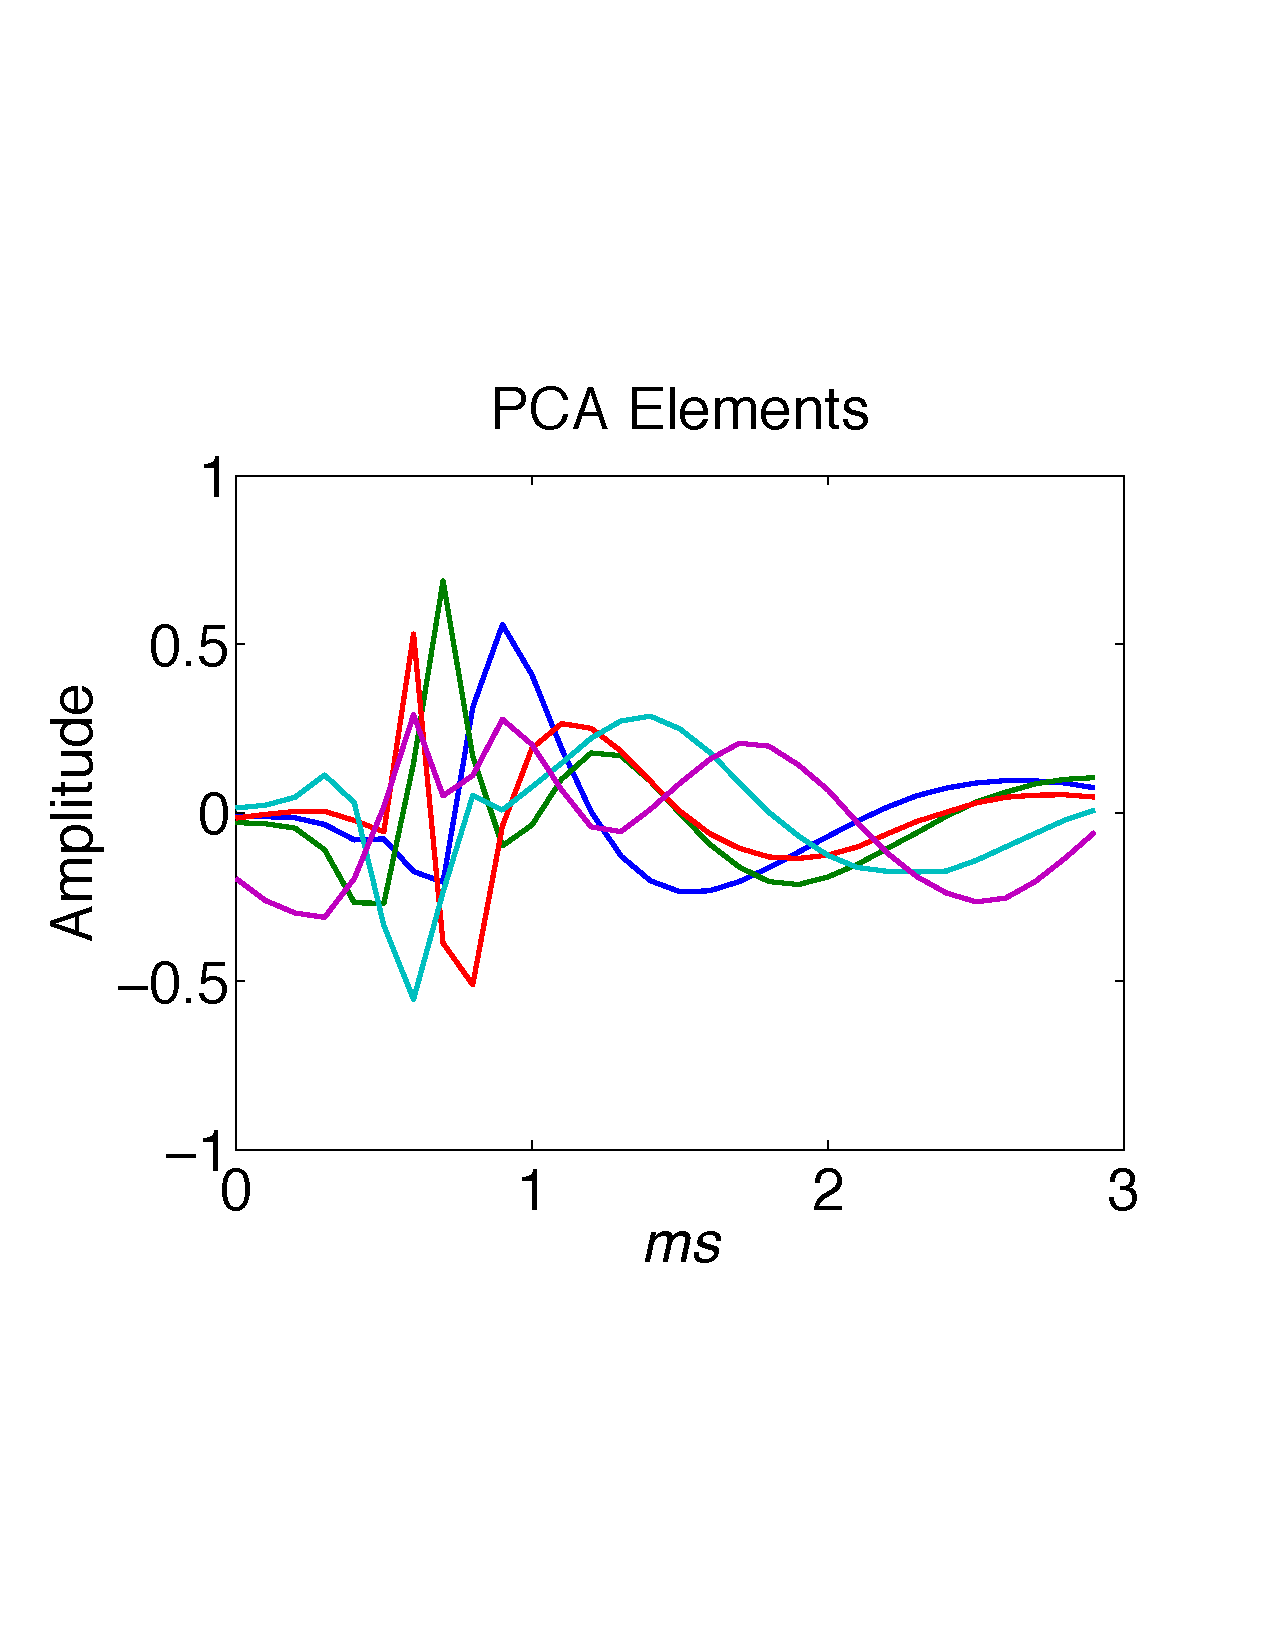
\includegraphics[width=\textwidth]{../figs/new/pcaelements.pdf}
\caption{}
\label{fig:ICold}
\end{subfigure}
\begin{subfigure}[b]{.3\textwidth}
% 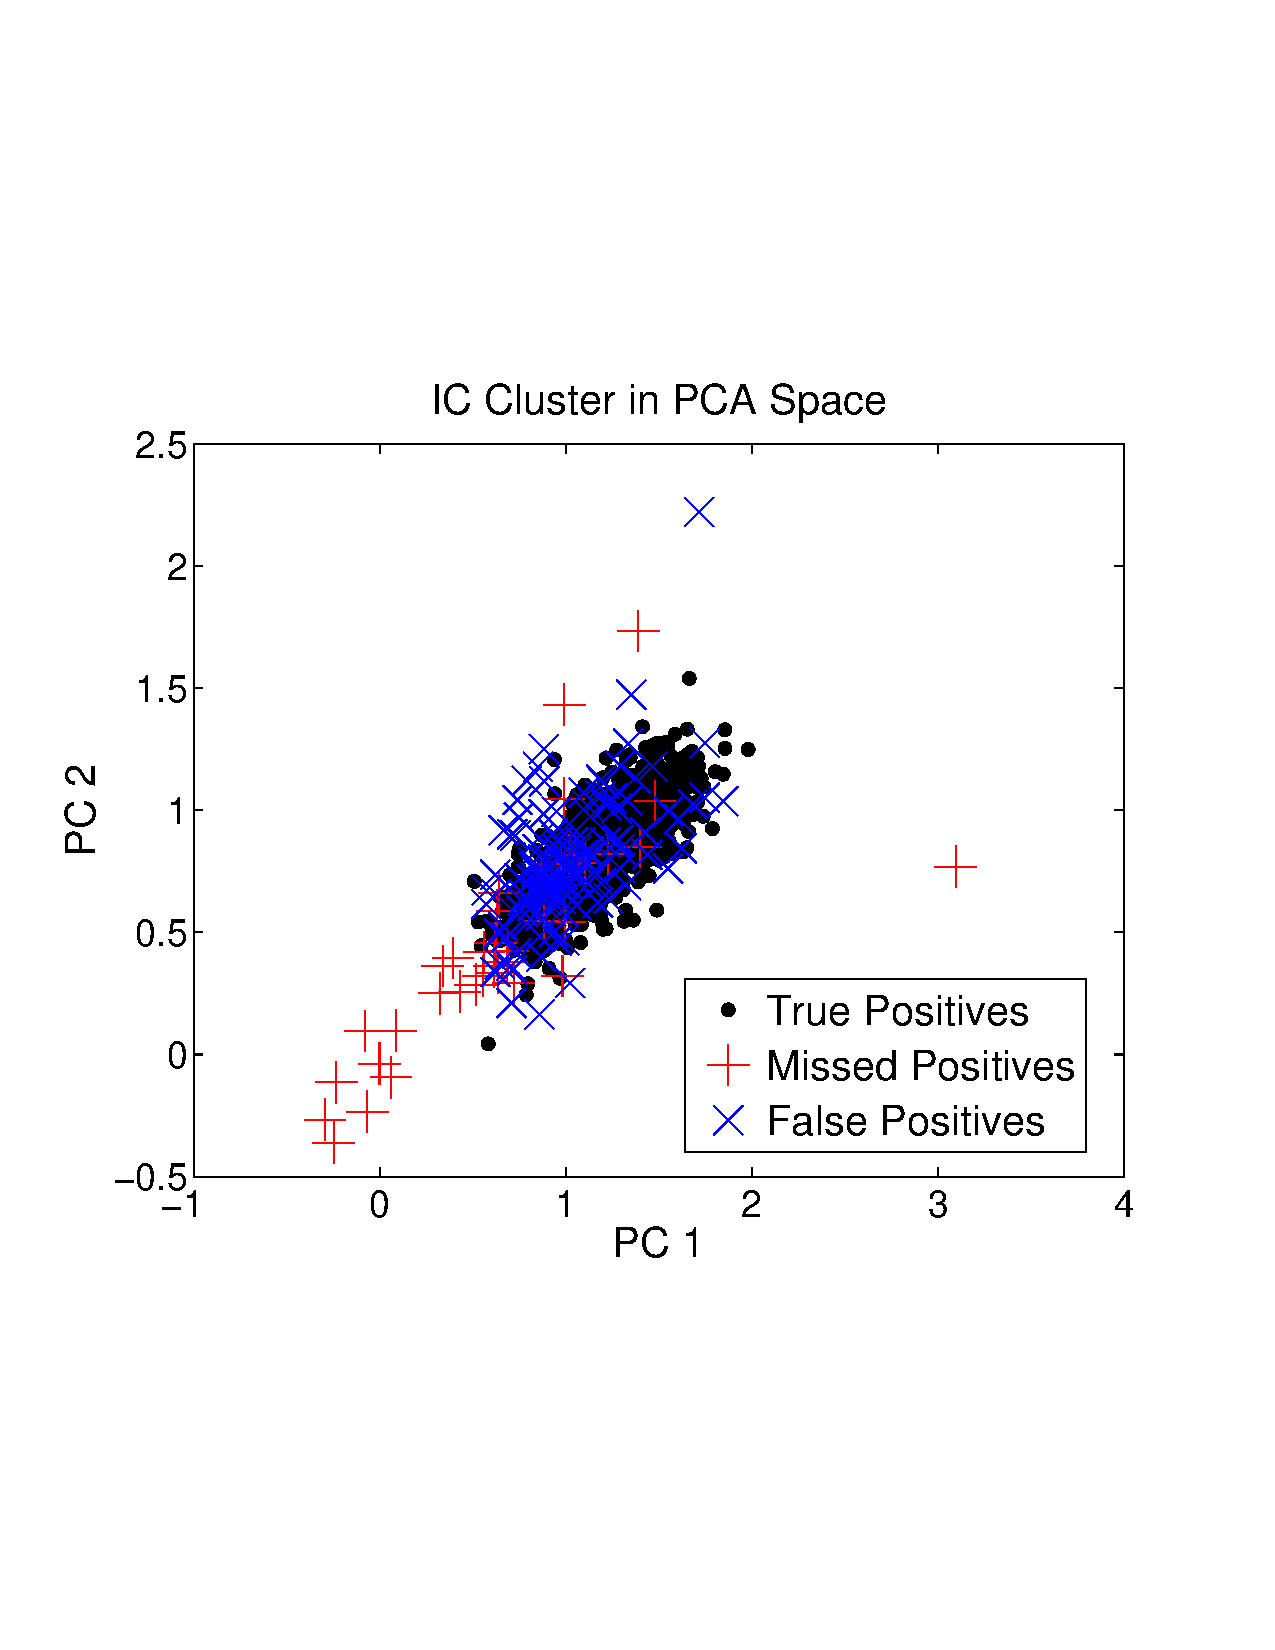
\includegraphics[width=\textwidth]{../figs/new/ICclusteroldpca.pdf}
\caption{}
\label{fig:ICold}
\end{subfigure}
\begin{subfigure}[b]{.3\textwidth}
% 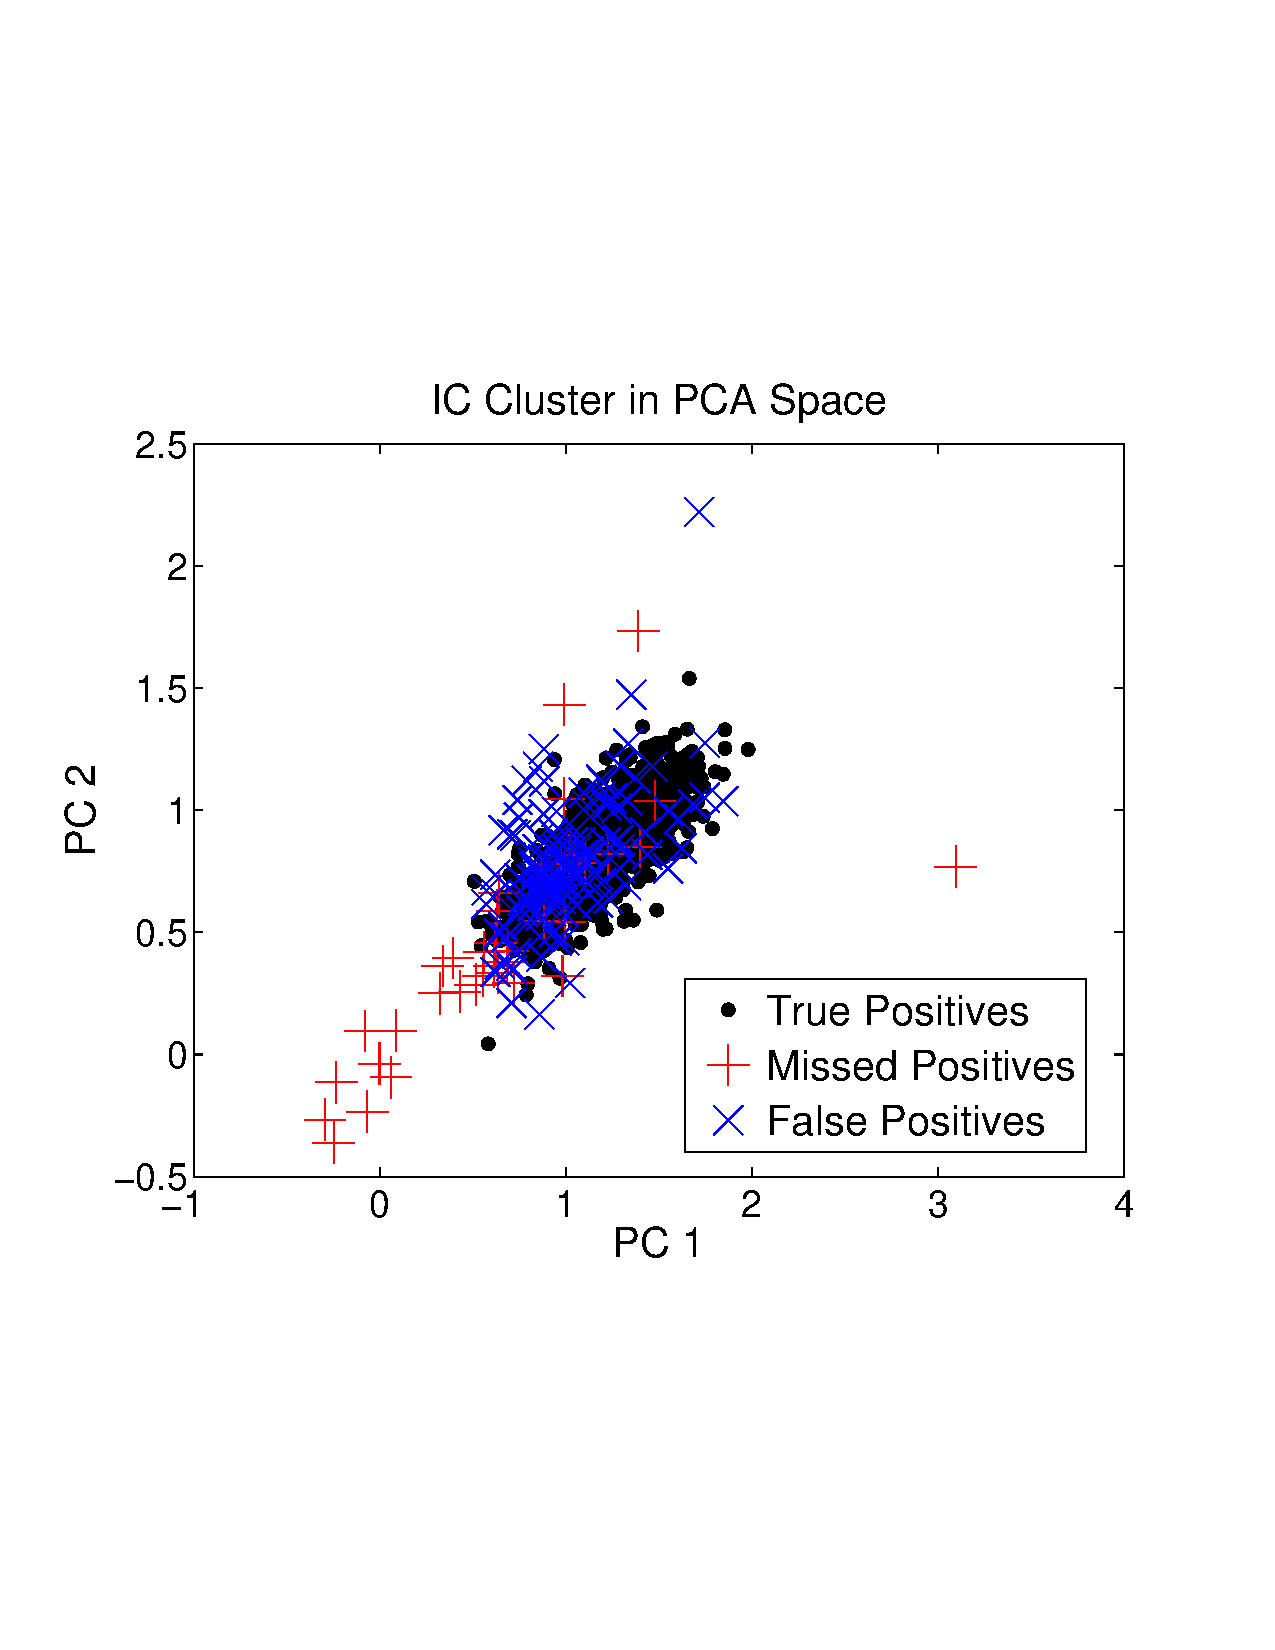
\includegraphics[width=\textwidth]{../figs/new/ICclusteroldpca.pdf}
\caption{}
\label{fig:ICold}
\end{subfigure}
\caption{\jovo{dictionary: (a) from first 5 secs, (b) from all data, (c) spectrum from all data which is cumsum/sum} 
} \label{fig:timing}
\end{figure}
\end{center}

\begin{figure}[htbp]
	\centering
		% 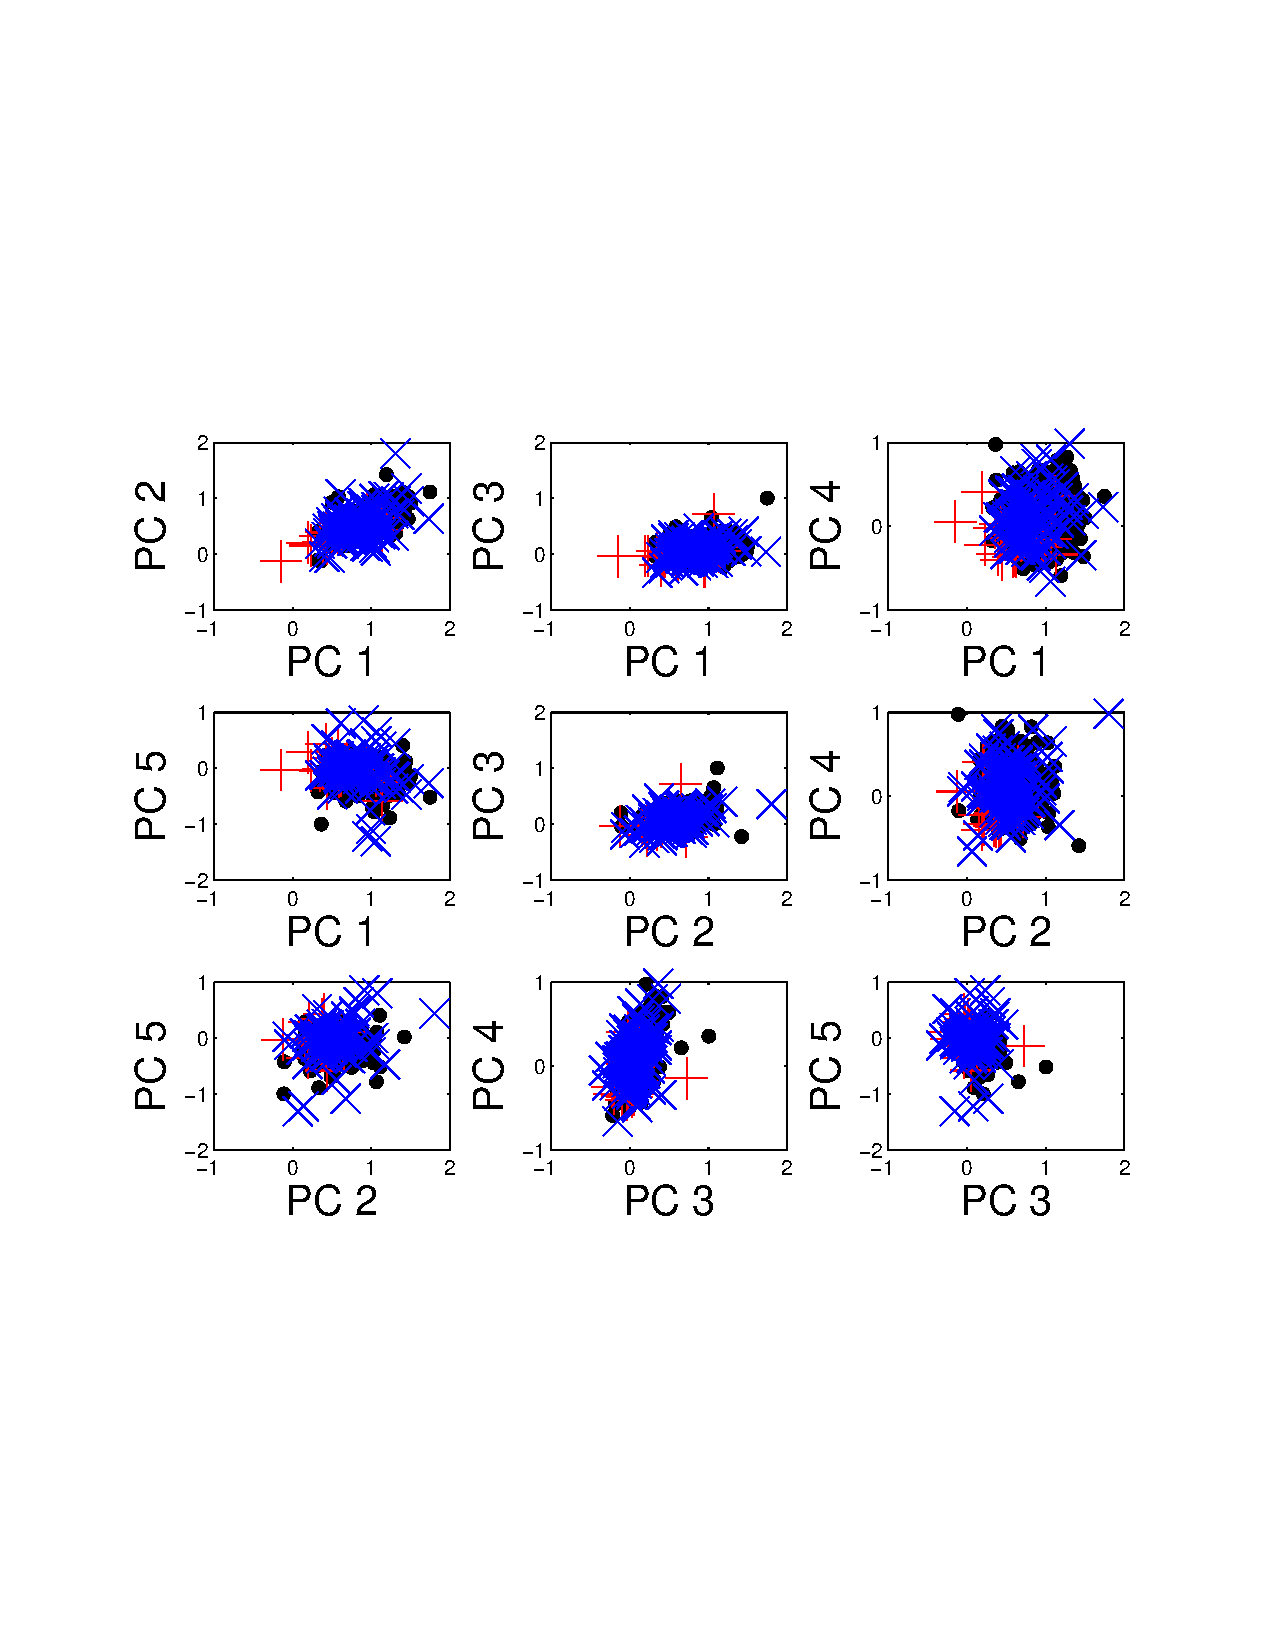
\includegraphics[height=3in]{../figs/new/pairs.pdf}
	\caption{(a) This shows the average number of true positives versus the average number of false positives in the intracellular cluster for 2 minute segments of the 4 minutes of the experiment.  \smug\ does better than    \jovo{let's make the symbols different for the different methods.  also, let's make the axes in terms of percentages, rather than raw numbers.} }
	\label{fig:asdf}
\end{figure}


\begin{figure}[htbp]
	\centering
		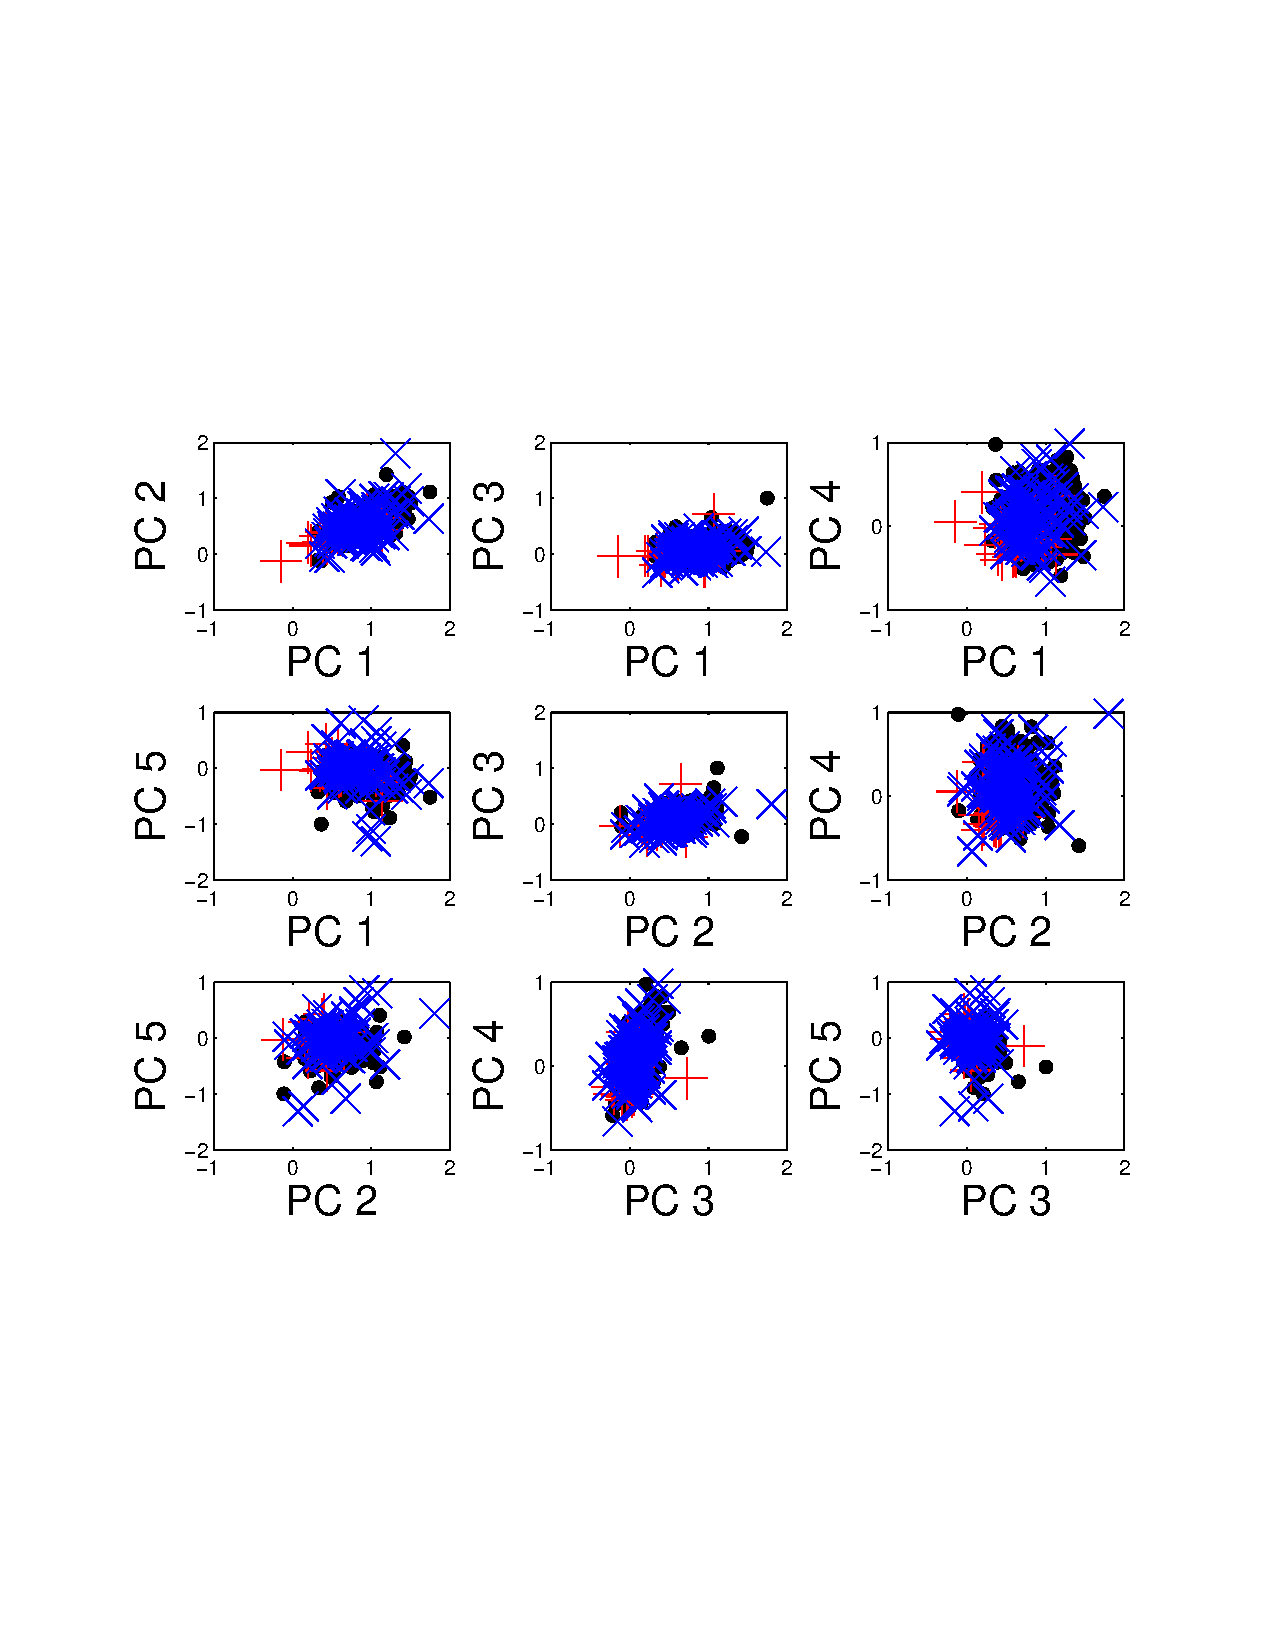
\includegraphics[height=3in]{../figs/new/pairs.pdf}
	\caption{caption}
	\label{fig:pairs}
\end{figure}



\begin{figure}[htbp]
	\centering
		% 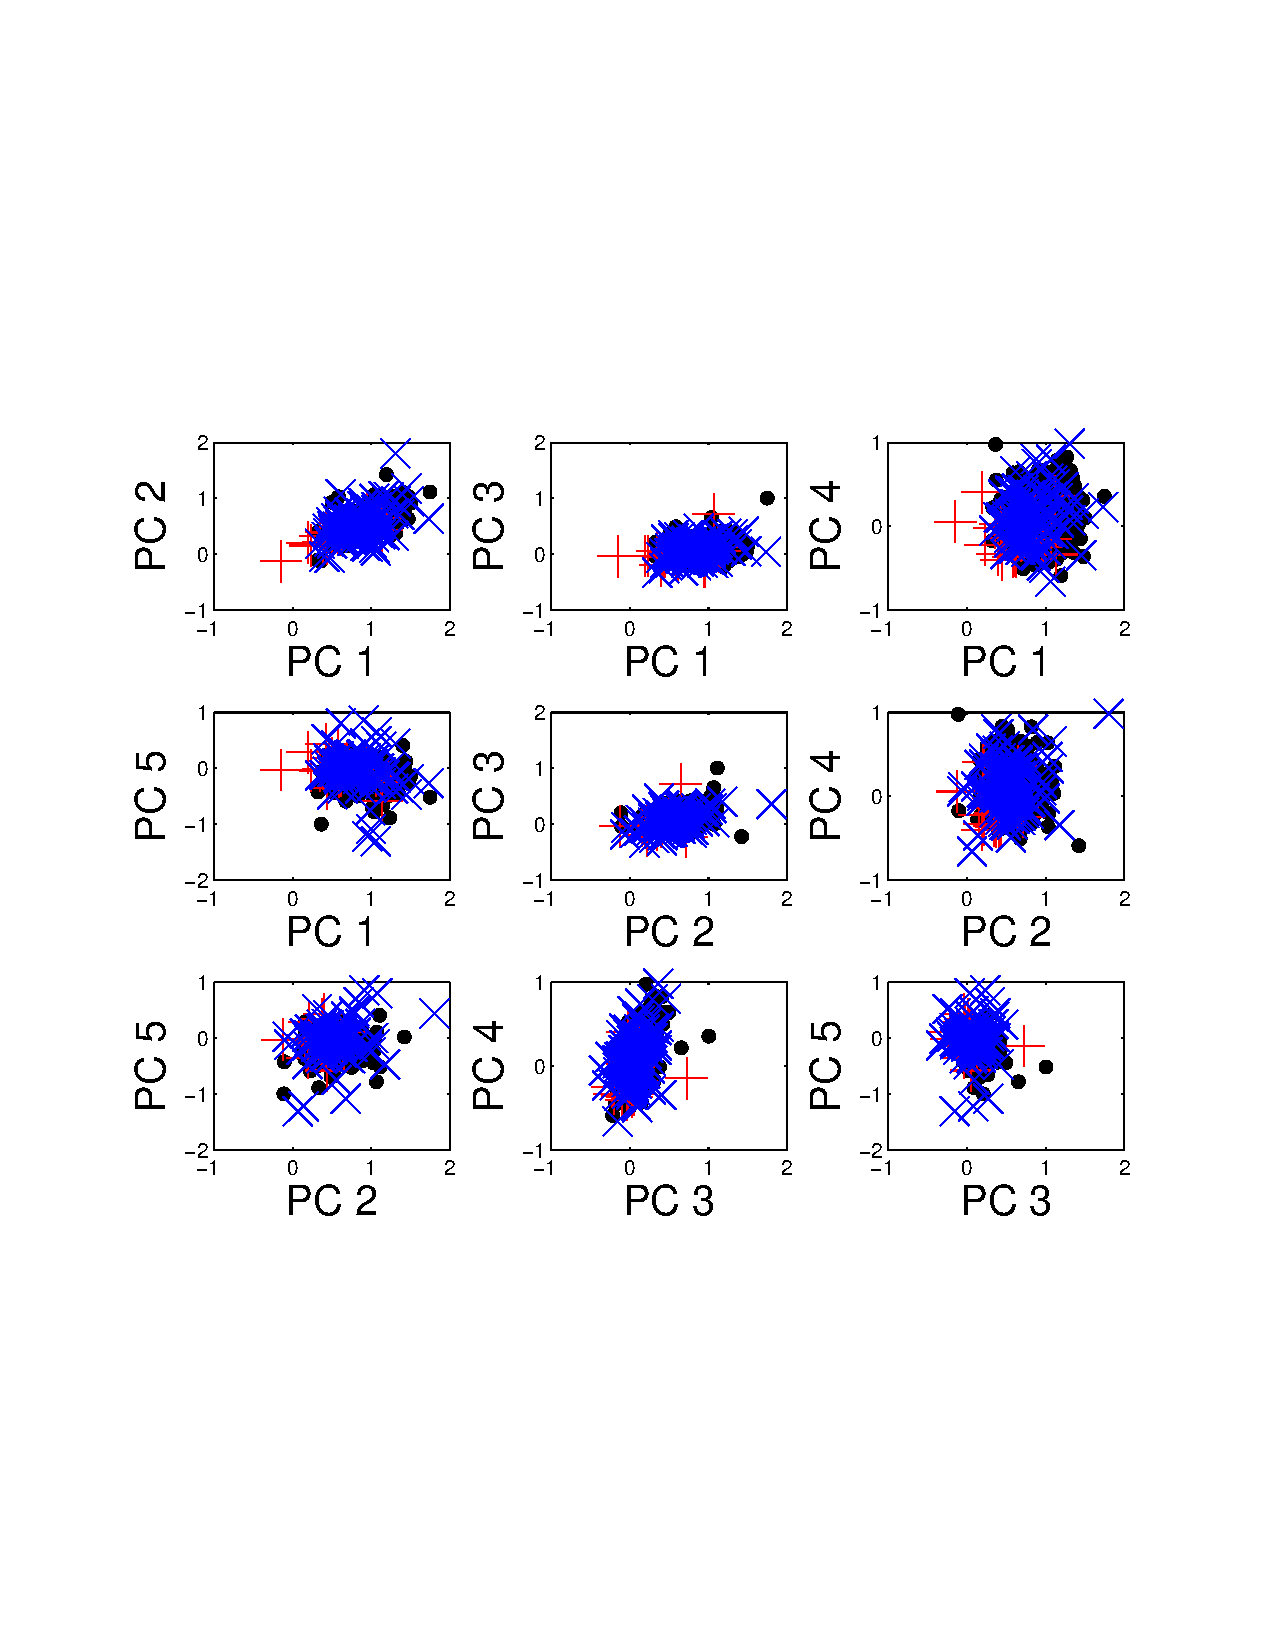
\includegraphics[height=3in]{../figs/new/pairs.pdf}
	\caption{(a) intracellular waveform shape over time (b) and in PC space.}
	\label{fig:pairs}
\end{figure}



\begin{center}
\begin{figure}
\begin{subfigure}[b]{.12\textwidth}
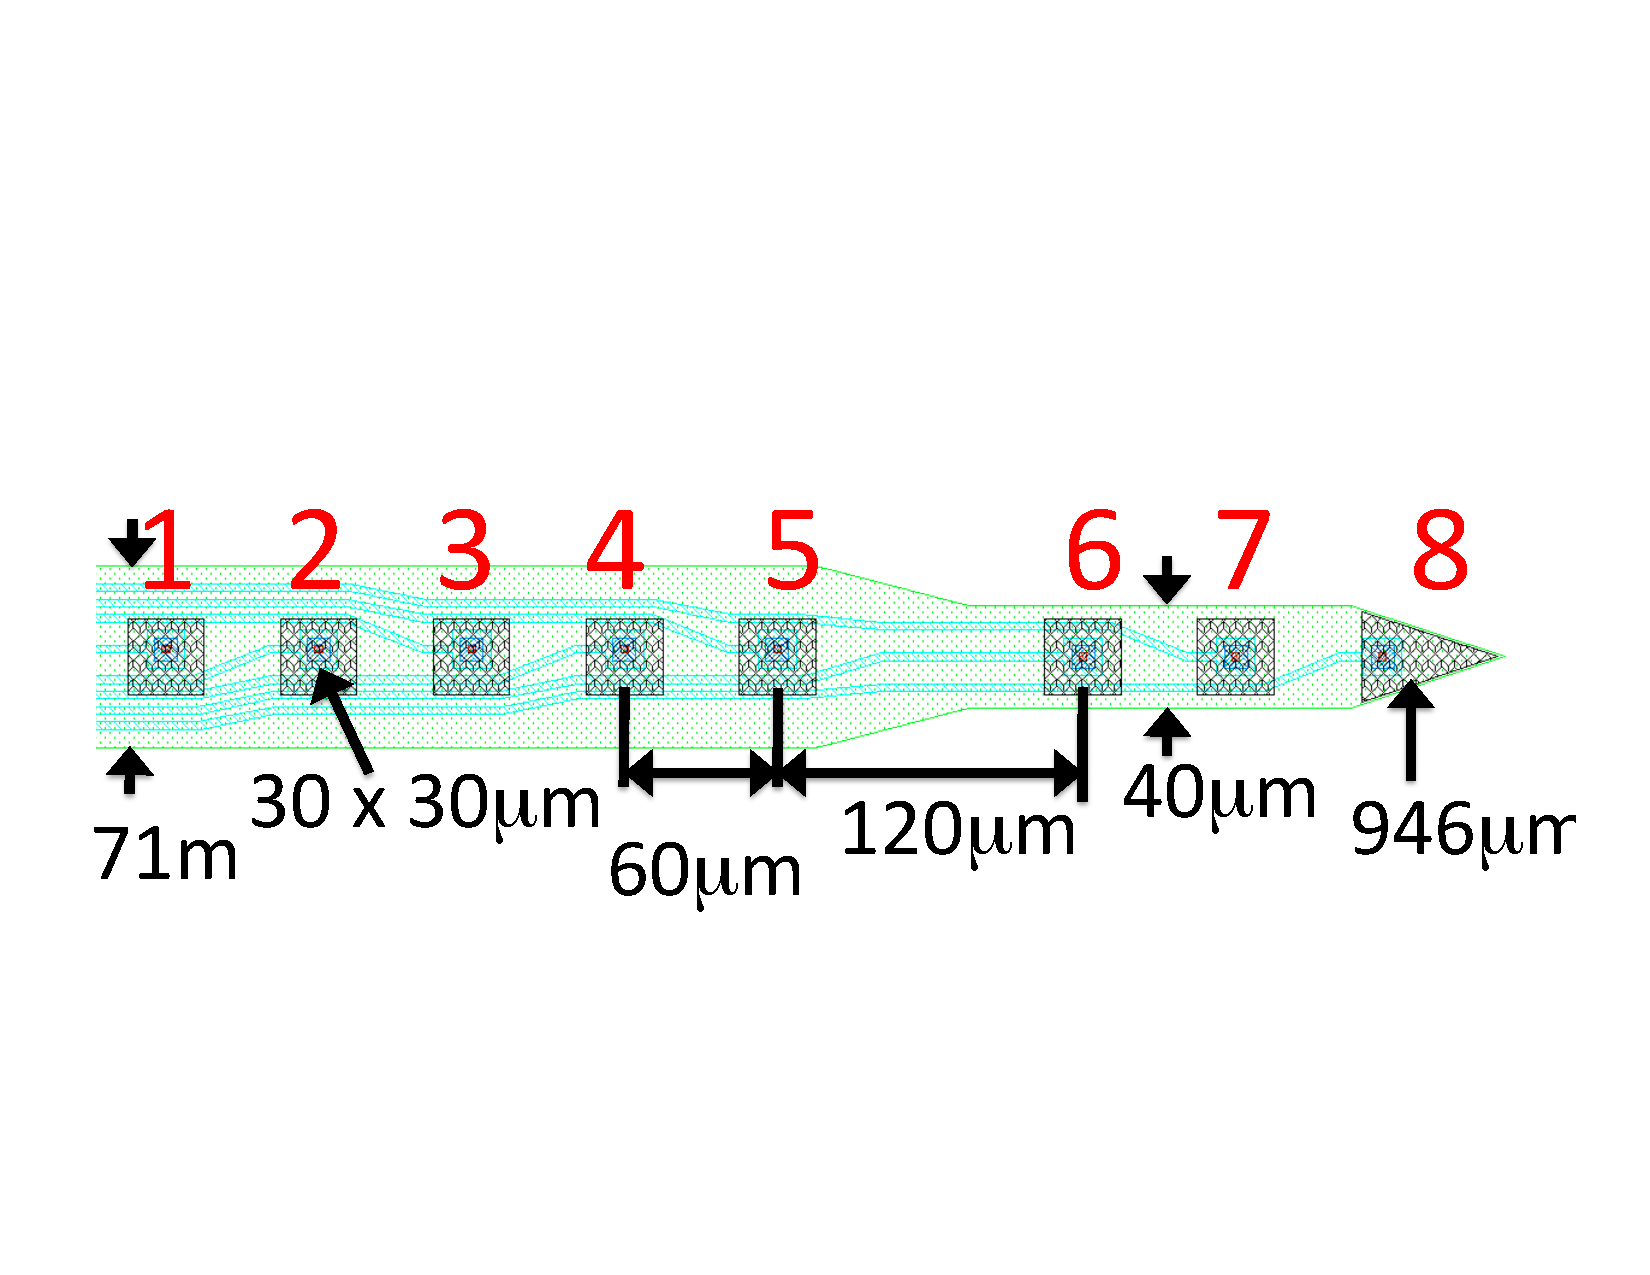
\includegraphics[width=0.8\textwidth]{../figs/8dev}
\caption{}
\label{8dev}
\end{subfigure}
\begin{subfigure}[b]{.28\textwidth}
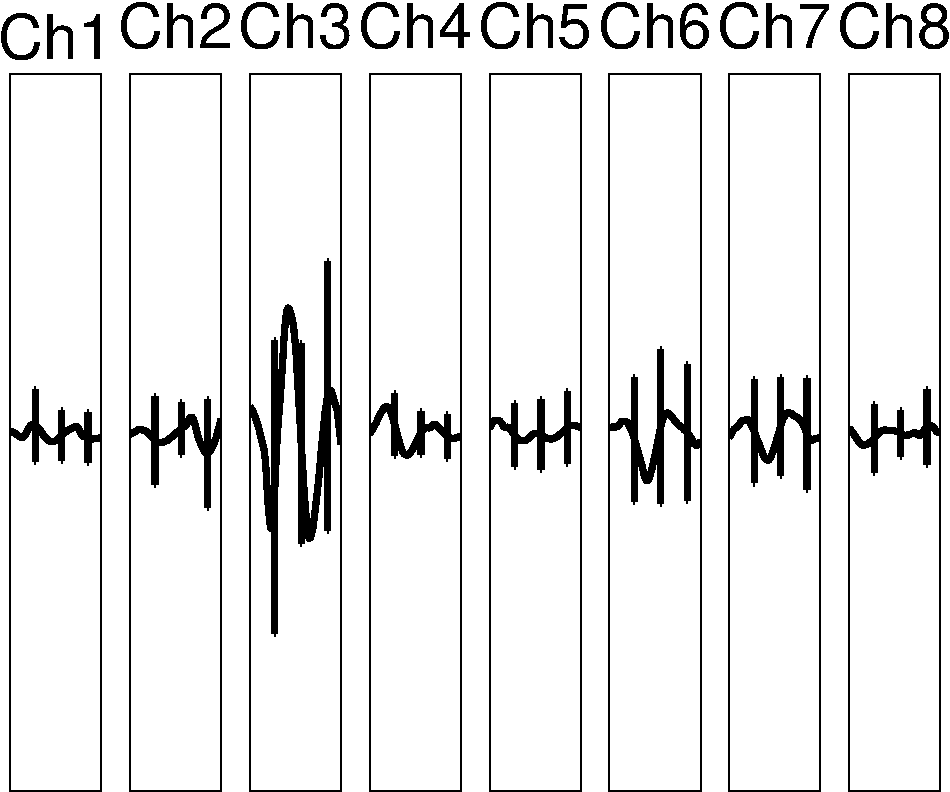
\includegraphics[width=\textwidth]{../figs/8devim/clus3}
\caption{}
\label{ex81}
\end{subfigure}
\begin{subfigure}[b]{.28\textwidth}
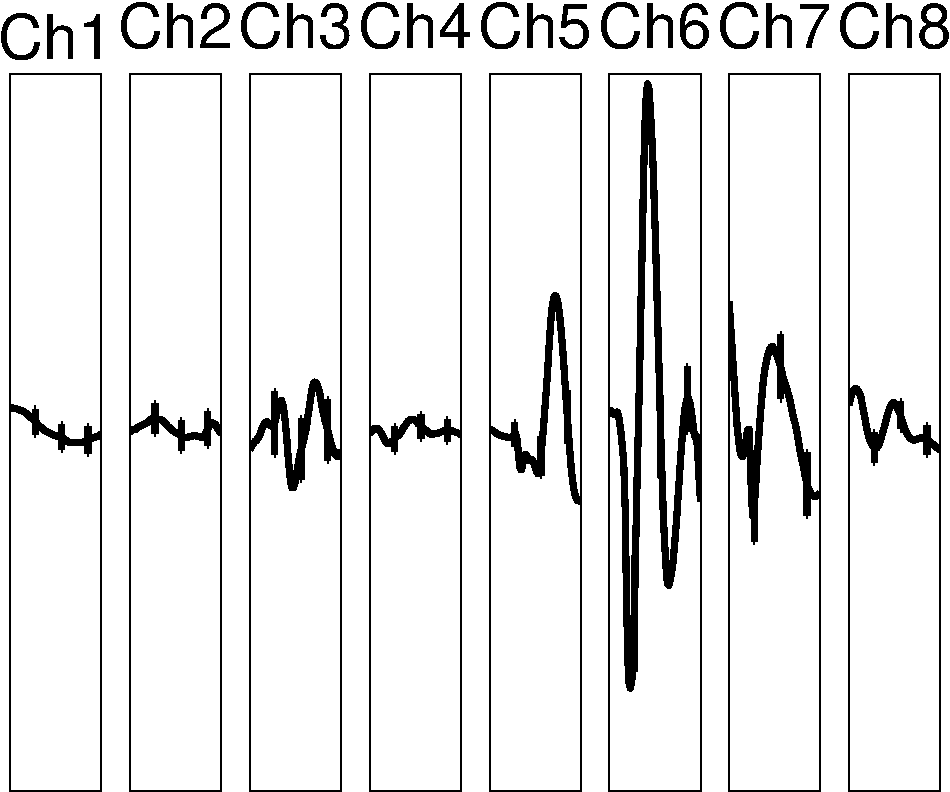
\includegraphics[width=\textwidth]{../figs/8devim/clus9}
\caption{}
\label{ex82}
\end{subfigure}
\begin{subfigure}[b]{.28\textwidth}
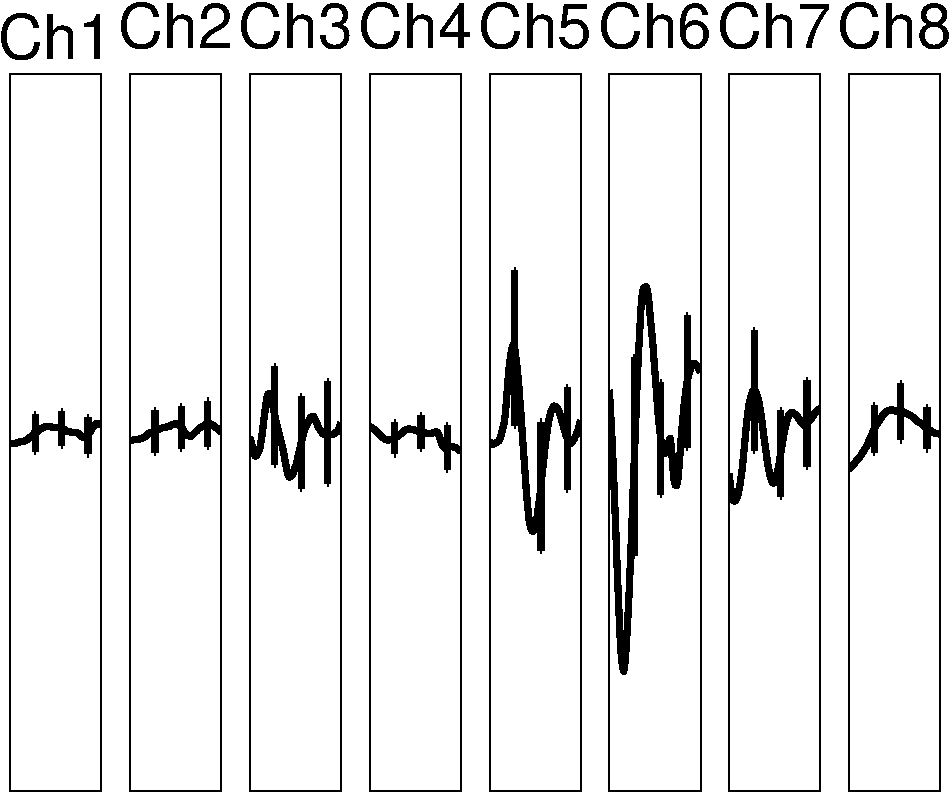
\includegraphics[width=\textwidth]{../figs/8devim/clus6}
\caption{}
\label{ex83}
\end{subfigure}
\caption{
\smug\ multielectrode performance.
(a) 8 electrode device showing local proximity of electrodes with channel indexes in large, red numbers. (b,c,d) Top three most prevalent waveforms.  Each waveform shape is 2 ms long.
} \label{sfig:8}
\end{figure}
\end{center}



\begin{center}
\begin{figure}[h!]
\begin{subfigure}[b]{.5\textwidth}
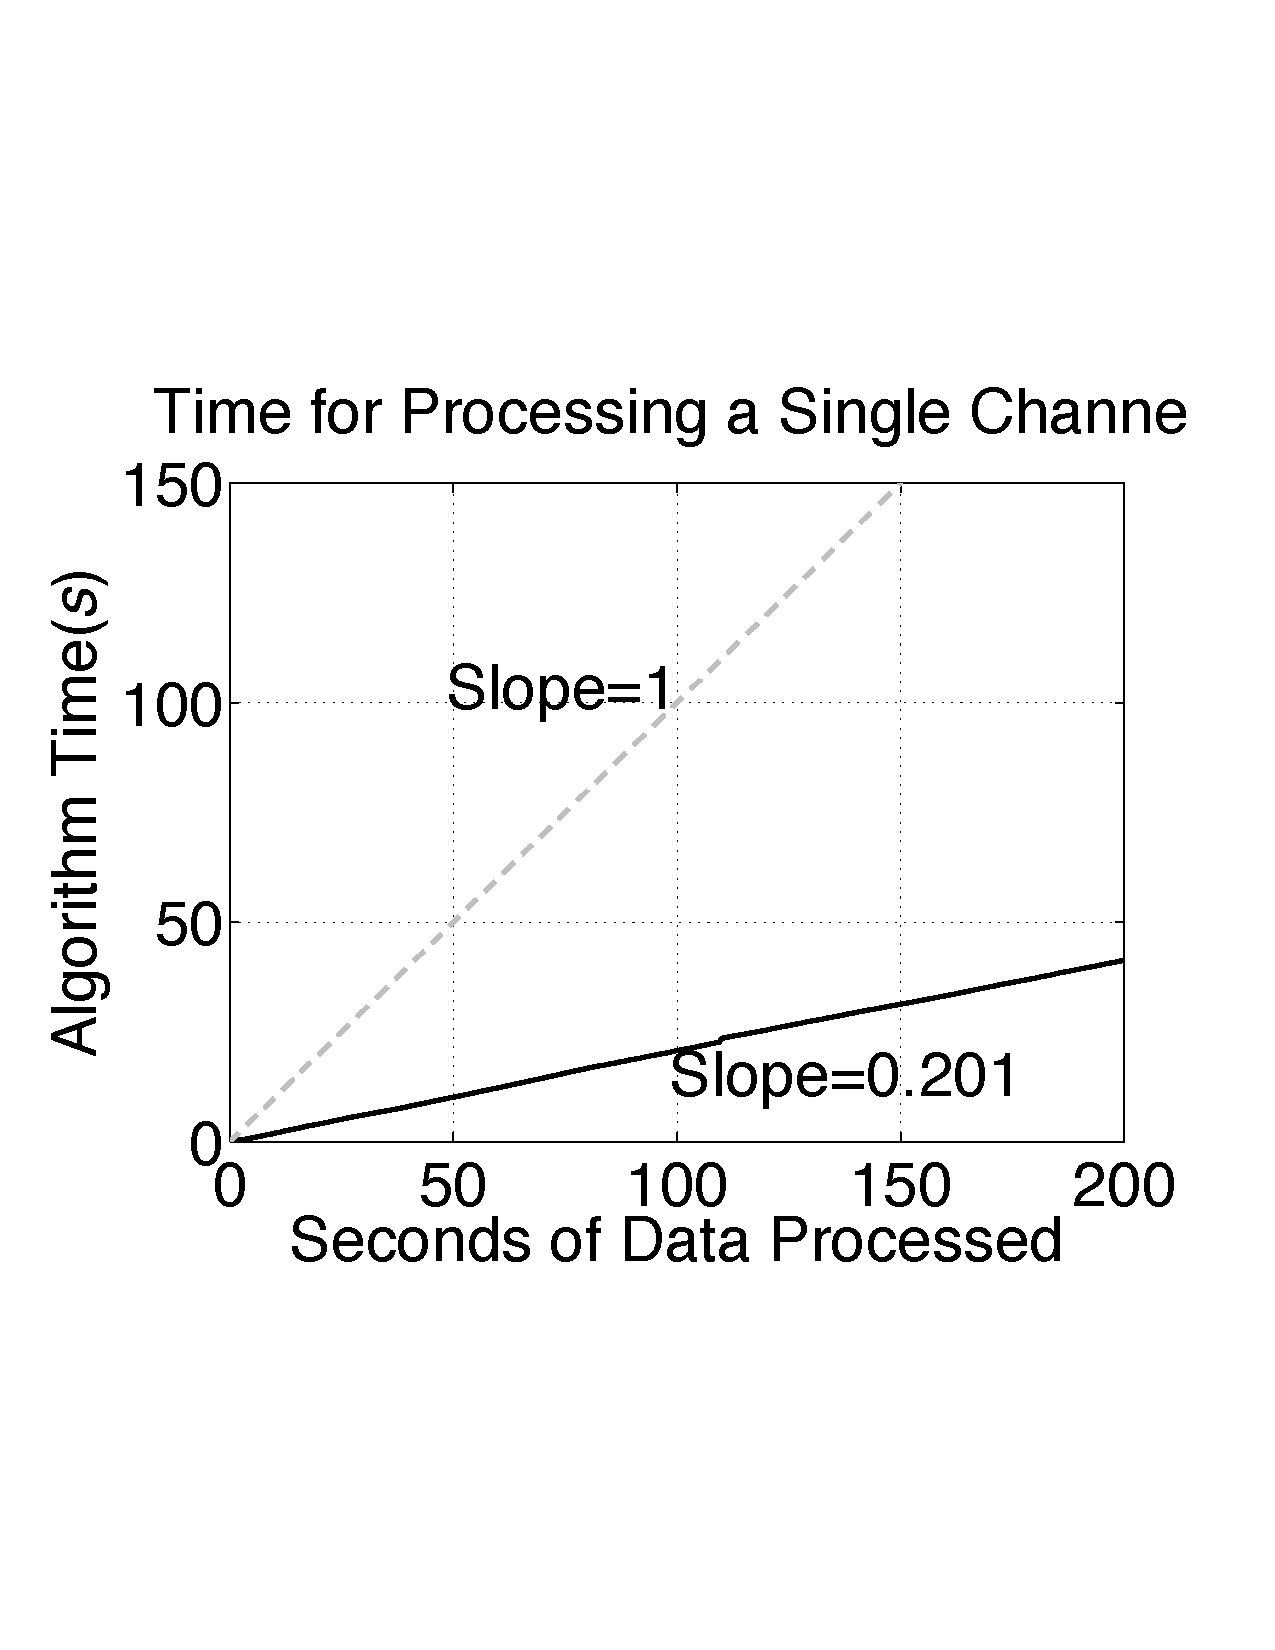
\includegraphics[width=\textwidth]{../figs/new/timingsinglechannel.pdf}
\caption{}
\label{fig:ICold}
\end{subfigure}
\begin{subfigure}[b]{.5\textwidth}
% 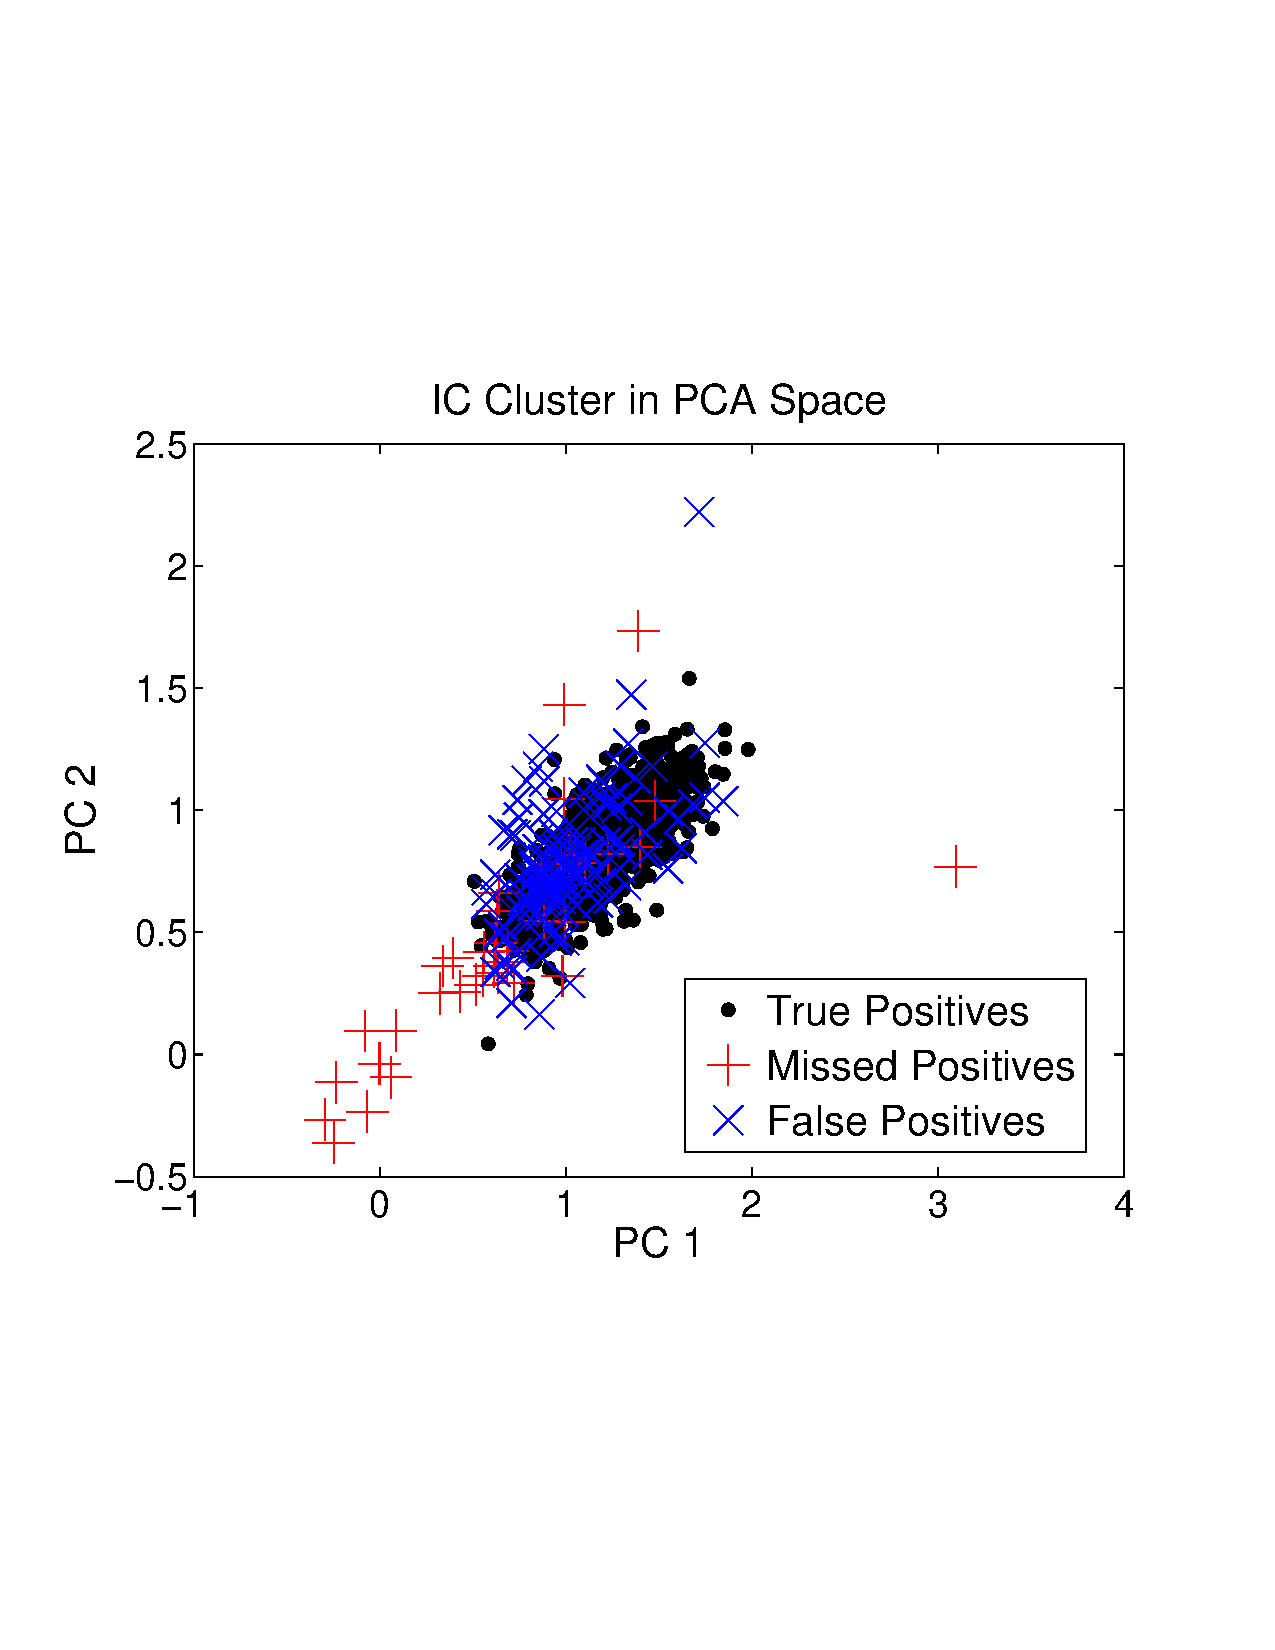
\includegraphics[width=\textwidth]{../figs/new/ICclusteroldpca.pdf}
\caption{}
\label{fig:ICold}
\end{subfigure}
\caption{\jovo{timing plots: (a) line (can we put a line on there for 4 channels too?), (b) notched boxplots. } 
} \label{fig:timing}
\end{figure}
\end{center}




\end{document}















